% FILE:    thesis_main.tex 
% AUTHOR:  Symon Stowe 
% DATE:    2020-01-06
%--------------------------------------------------------
% !TEX program = lualatex
% !BIB program = biber

% Define style of document
%\documentclass[12pt,twoside]{report}
\documentclass[12pt]{report}
\usepackage{amsmath} 
\usepackage{wasysym}
\usepackage{amssymb}
\usepackage{amsbsy}
\usepackage{graphicx}
\usepackage{multirow}
\usepackage{tikz}
\usepackage[linesnumbered,ruled,vlined]{algorithm2e}

% BIBER
\usepackage{csquotes}
\usepackage[american]{babel}
\usepackage[
backend=biber,
style=apa,
giveninits=true,
doi=false,
isbn=false,
url=false,
citestyle=authoryear,
maxbibnames=19,
apamaxprtauth=99,
maxcitenames=2,
uniquename=false,
uniquelist=false
]{biblatex}

\DeclareLanguageMapping{american}{american-apa}

\renewbibmacro*{name:andothers}{% Based on name:andothers from biblatex.def
  \ifboolexpr{
    test {\ifnumequal{\value{listcount}}{\value{liststop}}}
    and
    test \ifmorenames
  }
    {\ifnumgreater{\value{liststop}}{1}
       {\finalandcomma}
       {}%
     \andothersdelim\bibstring[\emph]{andothers}}
    {}}
\addbibresource{refs.bib}
\newcommand{\citeauthorandyear}[2][]{
   \citeauthor{#2} (\citeyear[#1]{#2})}
\renewcommand*{\nameyeardelim}{\addcomma\space} % Remove this line if you don't want the comma in citations
\DeclareCiteCommand{\citeyear}
    {}
    {\bibhyperref{\printfield{year}}}
    {\multicitedelim}
    {}

% Shortcuts for the perfusion paper
\newcommand{\PVi}{{\rm P_{Vf}}}
\newcommand{\PAa}{{\rm P_{At}}}
\newcommand{\PAi}{{\rm P_{Af}}}
\newcommand{\PVa}{{\rm P_{Vt}}}
\newcommand{\PBi}{{\rm P_{B}}}
\newcommand{\yB}{\mathbf{y}}
%\newcommand{\vB}{\mathbf{v}}
\newcommand{\uB}{\mathbf{u}}
\newcommand{\xB}{\mathbf{x}}
\newcommand{\xH}{\hat{\mathbf{x}}}
\newcommand{\nB}{\mathbf{n}}
%\newcommand{\CB}{\mathbf{C}}
\newcommand{\FB}{\mathbf{F}}
%\newcommand{\JB}{\mathbf{J}}
\newcommand{\DB}{\mathbf{D}}
\newcommand{\EX}{\mathrm{E}}
\newcommand{\IB}{\mathbf{I}}
\newcommand{\LB}{\mathbf{L}}
\newcommand{\MB}{\mathbf{M}}
\newcommand{\RB}{\mathbf{R}}
\newcommand{\qB}{\mathbf{q}}
\newcommand{\QB}{\mathbf{Q}}
%\newcommand{\VB}{\mathbf{V}}
\newcommand{\WB}{\mathbf{W}}
\newcommand{\sG}{\boldsymbol{\sigma}}
\newcommand{\gG}{\boldsymbol{\gamma}}
\newcommand{\GG}{\boldsymbol{\Gamma}}
\newcommand{\SG}{\boldsymbol{\Sigma}}
\newcommand{\LG}{\boldsymbol{\Lambda}}
\newcommand{\VB}{{\mbox{\bf V}}}
\newcommand{\YB}{{\mbox{\bf Y}}}
\newcommand{\CB}{{\mbox{\bf C}}}
\newcommand{\JB}{{\mbox{\bf J}}} 
\newcommand{\vB}{{\mbox{\bf v}}}

\addto\captionsenglish{% Replace "english" with the language you use
\renewcommand{\contentsname}%
{Table of Contents}% change "Contents" (default) to "Table of Contents"
}

% Define a TODO and Comment
\newcommand{\TODO}[1]{ \textsf{\color{red}{{TODO: \\ #1}}} }
\newcommand{\COMMENT}[1]{ \textsf{\color{blue}{{COMMENT: #1}}} }

\usepackage{fancyref}    

% Define margins of document
\sloppy
\usepackage{geometry}
\geometry{verbose,letterpaper} %,tmargin=20mm,bmargin=20mm,lmargin=20mm,rmargin=20mm}
% TODO how to we make the margins alternate like they should be in a book?
% TODO different print vs online versions with different margins?

% Set overall spacing
\usepackage{setspace}
\doublespacing
%\onehalfspacing   

% Shrink list spacing
% shrink the list environments
\usepackage{enumitem}
\setlist{noitemsep}
\setlist{nolistsep}

% Blank pages
\usepackage{afterpage}

\newcommand\blankpage{%
    \null
    \thispagestyle{empty}%
    %\addtocounter{page}{-1}%
    \newpage}

%List of abbreviations
\usepackage[acronym,nomain,nonumberlist]{glossaries}

\newacronym{eit}{EIT}{electrical impedance tomography}
\newacronym{mse}{MSE}{mean squared error}
\newacronym{fwhm}{FWHM}{full width half max}
\newacronym{sv}{SV}{stroke volume}
\newacronym{lv}{LV}{left ventricular}
\newacronym{svv}{SVV}{stroke volume variation}
\newacronym{co}{CO}{cardiac output}
\newacronym{fem}{FEM}{finite element model}
\newacronym{ct}{CT}{computed tomography}
\newacronym{mri}{MRI}{magnetic resonance imaging}
\newacronym{ards}{ARDS}{acute respiratory distress syndrome}
\newacronym{pet}{PET}{positron emission tomography}
\newacronym{spect}{SPECT}{single photon emission computed tomography}
\makeglossaries

% Include packages for manipulating figures/tables
\usepackage{epsfig} 

% Different font size in captions
\usepackage{./style/ccaption}
\captionnamefont{\bf \footnotesize}
\captiontitlefont{\footnotesize}
\captionwidth{130mm}
\changecaptionwidth

% Define page numbering scheme
\pagenumbering{roman}

% Make the table of contents clickable
\usepackage{hyperref}

% For the papers in appendix
\usepackage{pdfpages}

% Start of document
\begin{document}

% Define aliases
\newcommand{\pbox}{\parbox}

% Figures and Tables
\newtheorem{fig}{Figure}
\newtheorem{tab}{Table}

% Counter commands
\setcounter{page}{1}
\setcounter{chapter}{0}
\setcounter{secnumdepth}{4}
\setcounter{tocdepth}{3}

% BODY OF TEXT 
% Include the following files in main document
\normalsize

% START OF THESIS
% TITLE PAGE
% FILE:    title.tex
% AUTHOR:  Symon Stowe 
% DATE:    2020-01-06
%--------------------------------------------------------

% Suppress page number 
\thispagestyle{empty}
\begin{center}

%\vspace{-5mm}
\LARGE

\textbf{Electrical Impedance Tomography for Perfusion Imaging and Monitoring}

\vspace{6mm}
\large
by 

\vspace{-2mm}
\LARGE
Symon Stowe

\vspace{15mm}
\large
A thesis submitted in partial fulfillment of 
the requirements for the degree of

\vspace{12mm}
\large
Ph.D.\\

in \\

\vspace{1mm}
Biomedical Engineering\\

\vspace{12mm}
\large
Carleton University \\
Ottawa, Ontario\\

\vspace{12mm}
\large
\copyright~2021 \\
Symon Stowe
\end{center}

\thispagestyle{empty}
\cleardoublepage

% DEDICATION
\phantomsection
% Suppress page number
\thispagestyle{empty}

\mbox{  }
\begin{flushright}

\vspace{6cm}
\large

\textit{To ...}
\end{flushright}

\cleardoublepage

% LIST OF ABBREVIATIONS and SYMBOLS
%\addcontentsline{toc}{chapter}{List of Abbreviations}
%% FILE:    abbrev_body.tex
% AUTHOR:  Camille Gomez-Laberge 
% DATE:    12.04.2006
%
% (C) 2006, Camille Gomez-Laberge
% $Id: abbrev_body.tex 1302 2007-07-19 14:08:08Z cgomez $
%--------------------------------------------------------

\markboth{List of Abbreviations}
         {List of Abbreviations}

\subsection*{List of Abbreviations}

% BEGIN TABLE X.X
% SUBJECT: TABLE
\begin{table}[!h]
\vspace{5mm}
{\centering
\small
\begin{tabular}[t]{|c|c|}
\hline
\pbox[t]{30mm}{\centering \textbf{Abbreviation}} &
\pbox[t]{110mm}{\centering \textbf{Details}} \\
\hline

\pbox[t]{30mm}{\raggedright ASCII}&
\pbox[t]{110mm}{\raggedright American Standard Code for Information Interchange}\\

\pbox[t]{30mm}{\raggedright BLAST}&
\pbox[t]{110mm}{\raggedright Basic Local Alignment Search Tool}\\

\pbox[t]{30mm}{\raggedright BLOSUM}&
\pbox[t]{110mm}{\raggedright Blocks Substitution Matrices}\\

\pbox[t]{30mm}{\raggedright CASP}&
\pbox[t]{110mm}{\raggedright Critical Assessment of Methods of Protein Structure Prediction}\\

\pbox[t]{30mm}{\raggedright CATH}&
\pbox[t]{110mm}{\raggedright Class, Architecture, Topology, Homologous Superfamily}\\

\pbox[t]{30mm}{\raggedright CATH-PFDB}&
\pbox[t]{110mm}{\raggedright CATH Protein Family Database}\\

\pbox[t]{30mm}{\raggedright COG}&
\pbox[t]{110mm}{\raggedright Clusters of Orthologous Groups}\\

\pbox[t]{30mm}{\raggedright CORA}&
\pbox[t]{110mm}{\raggedright Conserved Residue Attributes}\\

\pbox[t]{30mm}{\raggedright DDBJ}&
\pbox[t]{110mm}{\raggedright DNA Databank of Japan}\\

\pbox[t]{30mm}{\raggedright DHDPS}&
\pbox[t]{110mm}{\raggedright Dihydropicolinate Synthetase}\\

\pbox[t]{30mm}{\raggedright DHS}&
\pbox[t]{110mm}{\raggedright Dictionary of Homologous Superfamilies}\\

\pbox[t]{30mm}{\raggedright DIVCLUS}&
\pbox[t]{110mm}{\raggedright Divide and Cluster}\\

\pbox[t]{30mm}{\raggedright DNA}&
\pbox[t]{110mm}{\raggedright Deoxyribonucleic Acid}\\

\pbox[t]{30mm}{\raggedright DSSP}&
\pbox[t]{110mm}{\raggedright Dictionary of Protein Secondary Structures}\\

\pbox[t]{30mm}{\raggedright EBI}&
\pbox[t]{110mm}{\raggedright European Bioinformatics Institute}\\

\pbox[t]{30mm}{\raggedright EC}&
\pbox[t]{110mm}{\raggedright Enzyme Commission}\\

\pbox[t]{30mm}{\raggedright EMBL}&
\pbox[t]{110mm}{\raggedright European Molecular Biology Laboratory}\\

\pbox[t]{30mm}{\raggedright EPQ}&
\pbox[t]{110mm}{\raggedright Error Per Query}\\

\pbox[t]{30mm}{\raggedright EVD}&
\pbox[t]{110mm}{\raggedright Extreme Value Distribution}\\

\pbox[t]{30mm}{\raggedright ExPASy}&
\pbox[t]{110mm}{\raggedright Expert Protein Analysis System}\\

\pbox[t]{30mm}{\raggedright FAD}&
\pbox[t]{110mm}{\raggedright Flavin Adenine Nucleotide}\\

\pbox[t]{30mm}{\raggedright FFF}&
\pbox[t]{110mm}{\raggedright Fuzzy Functional Forms}\\

\pbox[t]{30mm}{\raggedright FOD}&
\pbox[t]{110mm}{\raggedright Frequently Occurring Domain}\\

\pbox[t]{30mm}{\raggedright FORREST}&
\pbox[t]{110mm}{\raggedright Fold Recognition from Secondary Structures}\\

\pbox[t][9mm]{30mm}{\raggedright FSSP}&
\pbox[t]{110mm}{\raggedright Fold classification based on Structure-Structure alignment of Proteins}\\

\pbox[t]{30mm}{\raggedright HMM}&
\pbox[t]{110mm}{\raggedright Hidden Markov Models}\\

%\pbox[t]{30mm}{\raggedright HOMSTRAD}&
%\pbox[t]{110mm}{\raggedright Homologous Structure Alignment Database}\\

\pbox[t]{30mm}{\raggedright HSP}&
\pbox[t]{110mm}{\raggedright High Scoring Segment Pairs}\\

\pbox[t]{30mm}{\raggedright HSSP}&
\pbox[t]{110mm}{\raggedright Homology derived Secondary Structure of Proteins}\\

\pbox[t]{30mm}{\raggedright HTML}&
\pbox[t]{110mm}{\raggedright Hypertext Markup Language}\\

\pbox[t]{30mm}{\raggedright IMPALA}&
\pbox[t]{110mm}{\raggedright Integrating Matrix Profiles And Local Alignments}\\

\pbox[t]{30mm}{\raggedright ISL}&
\pbox[t]{110mm}{\raggedright Intermediate Sequence Library}\\

\pbox[t]{30mm}{\raggedright ISS}&
\pbox[t]{110mm}{\raggedright Intermediate Sequence Search}\\

\pbox[t]{30mm}{\raggedright JIPID}&
\pbox[t]{110mm}{\raggedright Protein Information Database of Japan}\\

\pbox[t]{30mm}{\raggedright LCS}&
\pbox[t]{110mm}{\raggedright Longest Continuous Segment}\\

\pbox[t]{30mm}{\raggedright MDM}&
\pbox[t]{110mm}{\raggedright Mutation Data Matrix}\\

\pbox[t]{30mm}{\raggedright MIPS}&
\pbox[t]{110mm}{\raggedright Martinsried Institute for Protein Sequences}\\

\pbox[t]{30mm}{\raggedright MISS}&
\pbox[t]{110mm}{\raggedright Multiple Intermediate Sequence Search}\\

\pbox[t]{30mm}{\raggedright MMDB}&
\pbox[t]{110mm}{\raggedright Molecular Modelling Database}\\

\hline
\end{tabular}
\par}
\centering
\end{table}
\vspace{5mm}
% END TABLE X.X

% BEGIN TABLE X.X
% SUBJECT: TABLE
\begin{table}[!h]
\vspace{5mm}
{\centering
\small
\begin{tabular}[t]{|c|c|}
\hline
\pbox[t]{30mm}{\centering \textbf{Abbreviation}} &
\pbox[t]{110mm}{\centering \textbf{Details}} \\
\hline

\pbox[t]{30mm}{\raggedright NAD}&
\pbox[t]{110mm}{\raggedright Nicotinamide Adenine Dinucleotide}\\

\pbox[t][9mm]{30mm}{\raggedright NC-IUBMB}&
\pbox[t]{110mm}{\raggedright Nomenclature Committee of the International Union of Biochemistry and Molecular Biology}\\

\pbox[t]{30mm}{\raggedright NCBI}&
\pbox[t]{110mm}{\raggedright National Center for Biotechnology Information}\\

\pbox[t]{30mm}{\raggedright NMR}&
\pbox[t]{110mm}{\raggedright Nuclear Magnetic Resonance}\\

\pbox[t]{30mm}{\raggedright NRDB}&
\pbox[t]{110mm}{\raggedright Non-redundant Database}\\

\pbox[t]{30mm}{\raggedright ORF}&
\pbox[t]{110mm}{\raggedright Open Reading Frame}\\

\pbox[t]{30mm}{\raggedright PAM}&
\pbox[t]{110mm}{\raggedright Point Accepted Mutation}\\

\pbox[t]{30mm}{\raggedright PCA}&
\pbox[t]{110mm}{\raggedright Principal Component Analysis}\\

\pbox[t]{30mm}{\raggedright PCR}&
\pbox[t]{110mm}{\raggedright Polymerase Chain Reaction}\\

\pbox[t]{30mm}{\raggedright PDB}&
\pbox[t]{110mm}{\raggedright Protein Data Bank}\\

\pbox[t]{30mm}{\raggedright PEDANT}&
\pbox[t]{110mm}{\raggedright Protein Extraction, Description and Analysis Tool}\\

\pbox[t]{30mm}{\raggedright PIR/PSD}&
\pbox[t]{110mm}{\raggedright Protein Information Resource / Protein Sequence Database}\\

\pbox[t]{30mm}{\raggedright PLP}&
\pbox[t]{110mm}{\raggedright Pyridoxal-5'-phosphate}\\

\pbox[t]{30mm}{\raggedright PRODOM}&
\pbox[t]{110mm}{\raggedright Protein Domain Database}\\

\pbox[t]{30mm}{\raggedright PSI-BLAST}&
\pbox[t]{110mm}{\raggedright Position Specific Iterated-BLAST}\\

\pbox[t]{30mm}{\raggedright RMSD}&
\pbox[t]{110mm}{\raggedright Root Mean Squared Deviations}\\

\pbox[t]{30mm}{\raggedright RNA}&
\pbox[t]{110mm}{\raggedright Ribonucleic Acid}\\

\pbox[t]{30mm}{\raggedright RPF}&
\pbox[t]{110mm}{\raggedright Ranked Pair File}\\

\pbox[t]{30mm}{\raggedright SAM}&
\pbox[t]{110mm}{\raggedright Sequence Alignment and Modelling}\\

\pbox[t]{30mm}{\raggedright SAS}&
\pbox[t]{110mm}{\raggedright Sequences Annotated by Structure}\\

\pbox[t]{30mm}{\raggedright SCOP}&
\pbox[t]{110mm}{\raggedright Structural Classification Of Proteins}\\

\pbox[t]{30mm}{\raggedright SMART}&
\pbox[t]{110mm}{\raggedright Simple Modular Architecture Research Tool}\\

\pbox[t]{30mm}{\raggedright SPARTACLUS}&
\pbox[t]{110mm}{\raggedright Superfamily Partition And Clustering}\\

\pbox[t]{30mm}{\raggedright SSAP}&
\pbox[t]{110mm}{\raggedright Sequential Structural Alignment Program}\\

\pbox[t]{30mm}{\raggedright SSE}&
\pbox[t]{110mm}{\raggedright Secondary Structure Element}\\

\pbox[t]{30mm}{\raggedright STAMP}&
\pbox[t]{110mm}{\raggedright Structural Alignment of Multiple Proteins}\\

\pbox[t]{30mm}{\raggedright SYSTERS}&
\pbox[t]{110mm}{\raggedright Systematic Re-searching}\\

\pbox[t]{30mm}{\raggedright TIM}&
\pbox[t]{110mm}{\raggedright Triosephosphate Isomerase}\\

\pbox[t]{30mm}{\raggedright TrEMBL}&
\pbox[t]{110mm}{\raggedright Translation of coding sequences from the EMBL database}\\

\pbox[t]{30mm}{\raggedright VAST}&
\pbox[t]{110mm}{\raggedright Vector Alignment Search Tool}\\

\pbox[t]{30mm}{\raggedright WU-BLAST}&
\pbox[t]{110mm}{\raggedright Washington University-BLAST}\\

\pbox[t]{30mm}{\raggedright WWW}&
\pbox[t]{110mm}{\raggedright World Wide Web}\\

\hline
\end{tabular}
\par}
\end{table}
\vspace{5mm}
% END TABLE X.X


%\addcontentsline{toc}{chapter}{List of Symbols}
%% FILE:    symbol_body.tex 
% AUTHOR:  Camille Gomez-Laberge 
% DATE:    12.04.2006
%
% (C) 2006, Camille Gomez-Laberge
% $Id: symbol_body.tex 1302 2007-07-19 14:08:08Z cgomez $
%--------------------------------------------------------

\markboth{List of Symbols}
         {List of Symbols}

\subsection*{List of Symbols}

% BEGIN TABLE X.X
% SUBJECT: TABLE
\begin{table}[!h]
\vspace{5mm}
{\centering
\small
\begin{tabular}[t]{|c|c|}
\hline
\pbox[t]{30mm}{\centering \textbf{Symbols}} &
\pbox[t]{110mm}{\centering \textbf{Details}} \\
\hline

\pbox[t]{30mm}{\raggedright $\alpha$}&
\pbox[t]{110mm}{\raggedright Gyromagnetic ratio of the Hydrogen atom}\\ 

\hline
\end{tabular}
\par}
\centering
\end{table}
\vspace{5mm}
% END TABLE X.X

% TODO pageskip TODO maybe!!

% ABSTRACT
\phantomsection
\addcontentsline{toc}{chapter}{Abstract}
% FILE:    abstract.tex
% AUTHOR:  Symon Stowe 
% DATE:    2020-01-21
%--------------------------------------------------------

% page number at bottom
\thispagestyle{plain}

%\section*{Summary}
\begin{abstract}
This thesis serves to show the background, methods, planned methods and timeline for the final thesis. 
The thesis will consist of 6 chapters, in introduction to give background and motivation for the research 
\end{abstract}

%\vspace{4mm}

\cleardoublepage

% ACKNOWLEDGEMENTS
%\markboth{Acknowledgements}{Acknowledgements}
\phantomsection
\addcontentsline{toc}{chapter}{Acknowledgements}
\thispagestyle{plain}

\section*{Acknowledgements}
 Write here

%\vspace{4mm}
\cleardoublepage

% CONTENTS, FIGURES, TABLES
\tableofcontents
\addcontentsline{toc}{chapter}{Contents}
\pagebreak

\markboth{List of Figures}{List of Figures}
\phantomsection
\addcontentsline{toc}{chapter}{List of Figures}
\listoffigures
\pagebreak

\markboth{List of Tables}{List of Tables}
\phantomsection
\addcontentsline{toc}{chapter}{List of Tables}
\listoftables
\pagebreak

\markboth{List of Acronyms}{List of Acronyms}
\phantomsection
\addcontentsline{toc}{chapter}{list of Acronyms}
\printglossary[type=\acronymtype,title=List of Acronyms]
\pagebreak

% Page Headings
% Chapter headings are in chapter files
\pagestyle{headings}
\pagenumbering{arabic}

% MAIN FILES
\section{Introduction}


\section{Background}
\chapter{Background}

\section{TODO}
this is short and needs a lot more detail and also figures.

This section briefly reviews the current techniques for lung perfusion and hemodynamic
monitoring, and provides a general overview 
of the state of 3D EIT as used for thoracic imaging and monitoring.

\subsection{Impedance Imaging}
Impedance imaging has been in use since the early 1900s in the geophysical community used as a technique to image
below the earth's surface~\parencite{Allaud1977}. 
In biomedical applications
EIT leverages electrical conductivity, permittivity and impedance properties of 
tissues and fluids within the body to compute conductivity distributions and generate images. 
Due to impedance differences associated with biological tissues and their physiological 
function~\parencite{Geddes1967,McAdams1995}
EIT has been proposed for a wide range of applications from thoracic monitoring to neuronal and 
brain imaging~\parencite{Holder1992,Frerichs2016}. 
% TODO in the thesis go into absolute imaging vs time difference imaging in depth here!!!
Imaging the absolute difference in tissue impedance is challenging due to the non-linear trajectory of 
electrical current, individual anatomy and difference in electrode contact impedance. 
Time difference EIT uses a reference frame to image the change in conductivity between 
two points in time and allows for imaging of functional activity such as the inflation of the lungs 
and the flow of blood.

Monitoring lung ventilation is one of the most
established clinical uses of 
\acrshort{eit}, presented initially by Barber and Brown~\parencite{Barber1984}.
EIT has also been used as a tool to monitor blood 
perfusion~\parencite{Brown1992} and hemodynamic parameters such as 
cardiac output~\parencite{Braun2018} and blood pressure~\parencite{Sola2011,Proenca2017}. 
While the spatial resolution of \acrshort{eit} is much lower than 
intermittent imaging techniques such as \acrfull{ct} or \acrfull{mri},
\acrshort{eit} can have a high temporal resolution enabling continuous or frequent 
monitoring without concerns regarding radiation exposure.
This thesis focuses on time difference EIT for thoracic hemodynamic imaging and monitoring applications. 

EIT is sensitive to the movement of blood in two main ways. First, a conductivity-contrasting 
bolus solution injected into a vein or artery can be used to image the transit of blood through the body
and second, the pulsatile changes in conductivity at the cardiac frequency can be isolated 
through digital filtering~\parencite{Leathard1994}.
This document proposes methods and techniques to identify and isolate these impedance variations
to monitor lung perfusion and 
aortic flow.

\subsubsection{Lung perfusion monitoring}
A perfusion scan is a technique for imaging the blood flow through the lungs
and when compared with ventilation images can be used to detect pulmonary embolisms
when a mismatch is identified. Clinically pulmonary perfusion is done using 
lung nuclear medical imaging such as \acrfull{spect}~\parencite{Parker2012}. Radio-isotopes are inhaled through a mask 
for ventilation imaging and injected into the blood to image pulmonary perfusion. 
Images taken on a gamma camera are compared to look for a mismatch between the ventilation
and perfusion distribution. This method of 
measuring lung perfusion is slow and exposes the subject to low-dose radiation.

EIT has been evaluated for its ability to measure cardiac output and
lung perfusion since the late 1980s~\parencite{Eyuboglu1989,Blottt1992,Brown1992,Frerichs2002}. 
Since then, various configurations of EIT have been evaluated~\parencite{Borges2012,Nguyen2015}.
Due to the speed and safety of measurement acquisition, EIT might be used to continuously monitor 
perfusion in subjects.

There are two main challenges with perfusion monitoring using EIT. First, impedance change due to ventilation 
is 10 times larger than the impedance change due to cardiac-frequency pulsatile activity~\parencite{Deibele2008}
and second, the pulsatile activity outside the lung region can overwhelm the lung perfusion signal~\parencite{Stowe2019}. 
There are several techniques available to mitigate the difference 
in magnitude such as: pausing ventilation; administering a 
conductivity-contrasting bolus through the heart and lungs via the jugular~\parencite{Frerichs2002};
and digital filtering to isolate activity at the cardiac frequency~\parencite{Leathard1994}. 

When breathing is paused, the signals based only on the cardiac activity can be more easily extracted. 
It was found that during apnoea the global impedance recorded with EIT measurements corresponded with stroke volume 
measured using the 
thermodilution method with a pulmonary arterial catheter~\parencite{Fagerberg2009}.
Ventilation perfusion ratios have been calculated during apnoea by comparing 
ventilation and perfusion signal amplitude with a specified region of 
interest~\parencite{Fagerberg2009a}.
There is some concern that the perfusion measured during apnoea may not accurately represent 
true perfusion during regular respiration as the apnoea impacts the regular respiratory cycle~\parencite{Leonhardt2012}.

Using the conductivity-contrasting bolus injection EIT perfusion imaging has been compared to 
SPECT measurements, and blood flow has been imaged from the right heart into the lungs and back into the left heart
using 5-10\% hypertonic saline~\parencite{Frerichs2002,Borges2012}. This technique is promising 
for imaging lung perfusion, but is slow and requires the placement of a venous catheter 
and repeated saline injections to obtain perfusion measures. 

The final method to calculate perfusion using EIT is through filtering to isolate the 
cardiac related signal. Previous work has shown that principal component analysis (PCA) 
can be used to separate ventilation and cardiac frequency signals and identify the component 
related to the heart~\parencite{Deibele2008}. Once the cardiac-frequency component of the 
EIT signal is identified the pulmonary component must also be isolated. Other than visual 
identification of the lung region or manually selecting a region of interest,
there are few good solutions for isolating pulsatile activity within the lung region.

The use of 3D configurations to differentiation between pulsatile activity 
in the heart and lungs could allow for an improved perfusion measure 
using EIT, and a means of continuously monitoring perfusion during ventilation.

\subsubsection{Aortic flow monitoring}

Continuous bedside monitoring appears to be one of the most
promising future applications of \acrshort{eit} due to the high 
temporal resolution, and concerns with other imaging modalities 
and the associated radiation 
exposure. 

%There are several hemodynamic parameters that are widely used to asses cardiovascular 
%health. One of the most used is cardiac output (CO), the amount of blood pumped through the
%heart in one minute.
%The two most used method is
%thermodilution using a Swan-Ganz catheter~\parencite{Khalil1963} in the pulmonary artery, 
%which determines CO by injecting a solution with a known temperature and 
%measuring the temperature change~\parencite{ReuterDaniel2010}. This method is considered the gold standard of 
%CO monitoring~\parencite{Joosten2017}.

Another potential use of EIT is to replace invasive monitoring techniques
such as catheterized measurements of pulmonary arterial pressure.
Recent studies have evaluated EIT as a method of determining 
pulmonary arterial pressure using pulse wave velocity in the 
descending aorta in 2D~\parencite{Braun2018a,Proenca2017,Proenca2016}.
EIT was a used in conjunction with ECG signals and shown to have a high correlation
with pulmonary arterial pressure values from from Doppler echocardiography~\parencite{Proenca2016}.

An analysis of hemodynamic measures using EIT found that measures of stroke 
volume and pulmonary arterial pressure are sensitive to electrode placement and
interference from pulmonary signals~\parencite{Braun2018a}. 
The solution proposed in this document uses an arrangement of internal electrodes placed in the 
esophagus adjacent to the aorta to increase the sensitivity to changes and improve detection 
accuracy and elimination of pulmonary signals.

Improving tracking and imaging of the aorta is also important because it
has additional clinical uses: it  can be used as a physiological landmark to identify
the back of the lungs, and can be used to continuously monitor blood pressure by
calculating the pulse transit time. 

\subsubsection{3D \acrshort{eit}}

The majority of EIT measurements are done with a single ring of external electrodes but 
in practice, electrical current cannot  be confined to a single plane
and using a two dimensional electrode configuration can significantly
impact the capabilities of \acrshort{eit}~\parencite{Rabbani1991}.
The use of 3D electrode configurations in \acrshort{eit}
was introduced in 1996~\parencite{Metherall1996} to overcome the 
inherent limitations of 2D measurements, but it is still not widely used today.
It is thought this is due to the increased complexity of 3D images
and the subsequent analysis~\parencite{Grychtol2019}.

It has been shown that externally placed 3D electrode configurations
consisting of two electrode planes
can improve the sensitivity distribution and image quality~\parencite{Grychtol2016},
but there is still limited sensitivity in the central-most regions 
of the chest.
The concept of using internal esophageal electrodes has been presented
previously~\parencite{Pilkington1989,Schuessler1995}
as a method to improve internal sensitivity 
and reconstruction quality,
but has not been widely used or simulated.
Several studies have shown that there may be several advantages to using an internal
electrode in \acrshort{eit} recordings; 
Measurements with an internal electrode have been 
shown to reconstruct images equally as well as configurations with 
twice as many external electrodes~\parencite{Schuessler1995},
and have shown an increase in sensitivity in a central region 
of interest~\parencite{Kwon2013,Czaplik2014,Farooq2014}.

\acrshort{eit} has been used clinically to monitor lung perfusion 
in an animal model~\parencite{Leonhardt2012,Nguyen2012}, and it is theorized that 
the use of an internal electrode for increased sensitivity may allow for 
imaging of blood flow in the aorta. 
There is great interest in monitoring cardiac parameters
using \acrshort{eit} to determine \acrfull{sv}~\parencite{Proenca2017,Braun2018}, and increased
sensitivity close to the heart also has the potential to improve
these measures.

While there have been some studies researching electrode placement for cardiac
imaging in 2D~\parencite{Noordegraaf1996} and 
3D electrode configurations~\parencite{Graham2007}, there has 
been little research into determining the optimal 3D external electrode configurations
for imaging the heart and aorta. 

Additionally when using alternate electrode configurations the current injection and 
measurement patterns must also be investigated. It has been suggested that  an internal electrode
in 2D
should not be used for current injection in asymmetrical models
as the reconstruction performance deteriorates~\parencite{NasehiTehrani2012}. 
It is unclear 
to what degree injection patterns affect the resulting sensitivity when
internal electrodes and alternate electrode arrangements are used in 3D.

This work aims to investigate internal and 
external electrode configurations for use in imaging blood movement 
in the thorax, and develop techniques to extract measures of 
aortic flow and lung perfusion from these reconstructions.

%\subsubsection{3D \acrshort{eit} image reconstruction}
%It has been shown that when the continuous boundary voltages of a surface are
%known, there is a unique solution to the inverse problem used to calculate internal 
%conductivity~\parencite{Calderon2006},
%but EIT uses discrete measurements of boundary voltage 
%and there is no unique solution. 
%
%In order to reconstruct EIT images prior information and smoothing 
%must be used to obtain a solution. There are several reconstruction methods used in 
%EIT including Tikhonov regularization~\parencite{Tikhonov1977} and 
%standardized methods for EIT such as GREIT~\parencite{Adler2009}.
%A version of GREIT for 3D reconstructions~\parencite{Grychtol2016}
%is used in this work.

\chapter{Comparison of bolus- and filtering-based EIT measures of lung perfusion in an animal model}

\begin{abstract}
    \emph{Objective:} Two main functional imaging approaches have been used to measure regional lung perfusion 
    using Electrical Impedance Tomography (EIT): venous injection of a hypertonic saline contrast
    agent and imaging of its passage through the heart and lungs, and digital filtering 
    of heart-frequency impedance changes over sequences of EIT images.
    This paper systematically compares filtering-based perfusion estimates and 
    bolus injection methods to determine to which degree they are related.
    \emph{Approach:} EIT data was recorded on 7 mechanically ventilated newborn lambs in which 
    ventilation distribution was varied through changes in posture
    between prone, supine, left- and right-lateral positions.
    Perfusion images were calculated using frequency filtering and ensemble averaging 
    during both ventilation and apnoea time segments for each posture to compare against 
    contrast agent-based methods using Jaccard distance score. 
    \emph{Main Results:} Using bolus-based EIT measures of lung perfusion as the reference
    frequency filtering techniques performed better than ensemble averaging
    and both techniques performed equally well across apnoea and ventilation data segments.
    \emph{Significance:} Our results indicate the potential for use of
    filtering-based EIT measures of heart-frequency activity as a non-invasive
    proxy for contrast agent injection-based measures of lung perfusion. 
\end{abstract}

\section{Introduction}

Electrical Impedance Tomography (EIT) uses electrical stimulation and measurements at electrodes on the
body surface to reconstruct images of internal conductivity
distribution and its changes.
The most common application of EIT, experimentally and clinically,
has been for imaging of the thorax~\parencite{Frerichs2017}.
Using a ring of electrodes around the chest, EIT is able to calculate
images of impedance changes in the abdomen.
Although most research has focused on
imaging of ventilation, there is significant interest in imaging
cardiovascular phenomena with EIT~\parencite{Adler2012,Leonhardt2012}. 

EIT has been evaluated for its ability to measure cardiac output and
lung perfusion since the early 90s~\parencite{Eyuboglu1989,Blottt1992,Frerichs2002}. % TODO FIX ACCENT
Since then, various configurations of EIT have been evaluated~\parencite{Borges2012,Nguyen2015}.
The effect of posture on EIT images
was evaluated by\citeauthorandyear{Reifferscheid2011}, who showed that changing posture
introduces a large and reproducible variability into ventilation distribution as imaged by EIT.
Based on results showing a common relationship between the effect of gravity and perfusion in both children and
adults~\parencite{Bhuyan1989},
in newborns we expect to see a comparable directional change in perfusion due to the changes in
posture.
Recently,\citeauthorandyear{Braun2018} evaluated EIT's ability to monitor
cardiac output, showing that EIT is more reliable for monitoring
cardiac output trends than absolute cardiac output.
EIT has also been investigated for
monitoring of systemic blood pressure~\parencite{Sola2011}, and 
for monitoring of pulmonary arterial pressure~\parencite{Proenca2017}.

EIT measurements are sensitive to blood movement in
two main ways. First, it is possible to image the transit of the
contrast agent through the heart and lungs via a conductivity-contrasting
bolus into the veins and second, through
digital filtering of the time series of EIT images at the heart
frequency~\parencite{Leathard1994}.
While multiple EIT measures of perfusion are used, their relationship is 
not well understood.
It is currently unclear to what degree pulsatile impedance changes
represent blood flow, and how
they limit the potential for heart-frequency filtering to correctly estimate
the true perfusion~\parencite{Nguyen2012}.

Injection of a contrast agent to measure regional lung perfusion has been compared with 
electron beam computed tomography (EBCT) and determined to be feasible 
for measuring perfusion across different animals~\parencite{Frerichs2002}.
Perfusion measurement via conductivity contrasts has the advantage of measuring the true perfusion,
but requires placement of a catheter to 
introduce the contrast agent.
Bolus-derived measurements cannot be made continuously because they rely
upon the circulation of a contrast agent. In addition, 
the accumulation of NaCl (the main conductivity contrast used)
over multiple injections
can lead to hypernatremia which limits the rate at which bolus
injections can be made.
 
Calculating the heart-frequency conductivity 
changes in the thorax offers the benefit of a continuous functional
measure calculated directly from EIT signals (possibly
in conjunction with a synchronization signal such as the ECG).
Heart-frequency EIT signals are typically an order of magnitude smaller than
ventilation signals; thus, when measurements are made during
tidal ventilation, a large period of data must be used
in order to reduce the ventilation signal. On the other hand,
measurements during apnoea can be used to eliminate the ventilation signal,
but for the safety of the patient the apnoea was limited to 30\,s.
In healthy human subject of less than one year old it 
takes a mean of 118\,s 
for the blood oxygen saturation levels to drop below
90\%~\parencite{Xue1996}, however
the length of safe apnoea is much shorter for the sick preterm infant.
The time period was chosen based on experience in the lab showing 
that 30\,s seconds was
not associated with bradycardia or desaturation to less than 90\% blood oxygen saturation.

There is a debate within the EIT community about the meaning of
heart-frequency EIT signals~\parencite{Frerichs2017, Adler2017a}. 
Not all perfusion results in a
cardiac-frequency change (for example, continuous blood flow in capillaries),
and
non-perfusion effects (for example, heart movement in the thoracic cavity)
can result in heart-frequency EIT signals.
This debate is reflected by the terminology 
-- perfusion vs.\ pulsatility.
Those who prefer ``pulsatility'' or ``heart-frequency fEIT image'' seek to emphasise that frequency
filtered signals are not ``perfusion'' (although they may be related).
While these pulsatility based EIT images are clearly not a direct measure of
perfusion, the signals appear to be useful and are often measured and 
reported~\parencite{Bartocci1999,Halter2008,Moens2014,Ericsson2016}. 
To the authors' knowledge, no systematic comparison of
frequency-based perfusion measures has been published.

The heart-frequency signal can be derived from
frequency filtering or ensemble averaging.
Frequency-filtering uses a filter to isolate the frequency of heart-frequency conductivity changes,
and was introduced by\citeauthorandyear{Blottt1992} and\citeauthorandyear{Leathard1994}. 
Frequency filtering is susceptible
to interference from ventilation when the heart rate is at a harmonic
of the breathing rate.
Ensemble averaging is another filtering approach which
averages signals at a synchronized time, for example at the QRS 
peak~\parencite{Bartocci1999, Deibele2008}. The impedance change due to each heart 
beat is aligned and averaged to give a single heart-related impedance change,
representative of all heart-beats in the segment.

In this paper, we are motivated to better understand the relationship between
lung perfusion and heart-frequency filtering measures, and between the various filtering
approaches used to determine heart-frequency components. Our questions are:
1) to what extent do heart-frequency filtering-based measures correspond to perfusion,
2) what are the advantages and disadvantages of different approaches
to heart-frequency filtering of EIT data, and 3) which techniques are recommended.
In our experimental protocol, we have selected posture-change 
to introduce changes in the regional distribution of lung perfusion.
These changes are then compared using bolus- and filtering-based
EIT measures.



\section{Methods}
\subsection{Overview}
Data were acquired as an additional protocol within 
a study to determine a baseline for 
lung damage due to gas ventilation in neonatal lambs. 
This is part of an effort to establish total liquid ventilation (TLV) as a less-injurious 
ventilation strategy for the delicate lungs of neonatal 
subjects~\parencite{Sage2018}. In order to induce changes in ventilation 
and perfusion patterns, 
posture changes were made between supine, prone, left and right lateral positions. 


\subsection{Animals}  \label{animals}
The study was conducted in accordance with the Canadian Council 
on Animal Care guidelines upon approval by the animal research ethics 
board of Universit\'e de Sherbrooke (protocol 417-17BR). 

Seven healthy neonatal lambs (2--4
days old and 2.95$\pm$0.27\,kg) were used.
Animals were anaesthetised (ketamin 10\,mg/kg IM at induction followed by 
propofol 100\,mcg/kg/min and ketamin 2\,mg/kg/h IV) and placed 
under mechanical gas ventilation with: peak inspiratory pressure 
(PIP) 15 cmH$_2$O, positive end-expiratory pressure (PEEP) 5 cmH$_2$O, 
respiratory rate (RR) of 60/min, and fractional concentration of O$_2$ in 
inspired gas (FiO$_2$) of 30\%.

A catheter was inserted into the carotid artery for blood gas and 
continuous blood pressure monitoring. A jugular venous access was inserted 
to inject the saline bolus for generating perfusion images. Each 
animal was shaved for placement of a custom EIT belt 
around the lower third of the sternum in the transverse plane.

For each animal a bolus injection protocol was used: 
1.5\,mL of 7.5\% saline was injected into the jugular vein
at a constant rate over approximately 2s.
Before each bolus, ventilation was stopped for ten seconds,
and a further twenty seconds of apnoea was maintained before
restarting ventilation.

After one hour of ventilation (for stabilization) EIT recordings were made 
during the position change procedure. Each lamb was rotated
onto its right side. Five minutes after turning
the subject, the bolus injection protocol was implemented.
The animal was then ventilated normally, remaining on the right side for 
an additional five minutes, before being positioned on the left side 
for 5 minutes of regular ventilation, followed by the bolus
injection protocol.

At 2 hours of ventilation, the position change procedure was repeated,
changing the positioning of the lamb from prone to supine as the bolus 
injection protocol was repeated and EIT recordings were captured.

\begin{figure}
\begin{flushright}
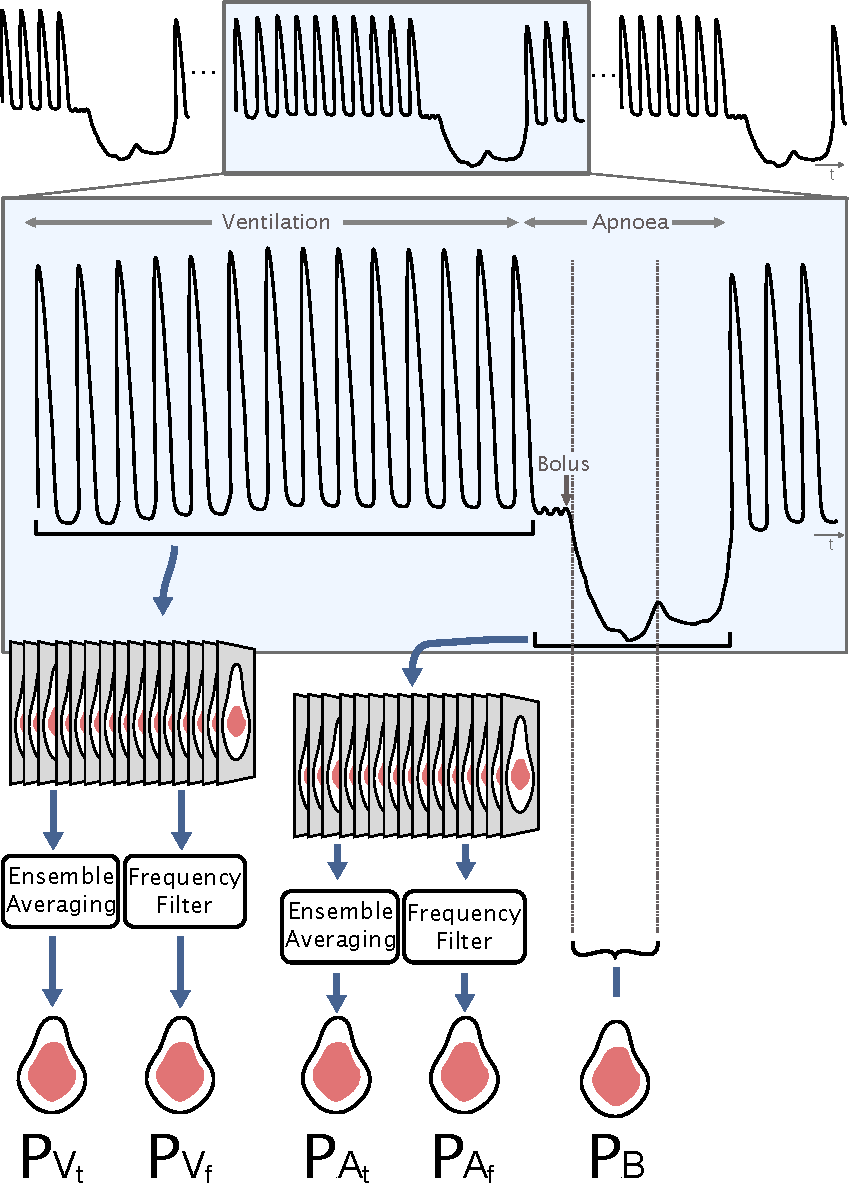
\includegraphics[width=0.8\textwidth]{chapter_2/imgs/fig-methodsOverview.pdf}
\end{flushright}
\caption{\label{fig:methods}%
This figure is a schematic overview of analysis methods for EIT perfusion. 
The upper
curve illustrates the global EIT signal during a period of ventilation
followed by apnoea and renewed ventilation. During apnoea a bolus
of conductivity contrasting saline is introduced. From these data
5 fEIT images are calculated:
$\PVa$: pulsatility (perfusion) image during ventilation, calculated
by ensemble averaging EIT data during ventilation;
$\PVi$: pulsatility (perfusion) image during ventilation, calculated
by frequency filtering EIT data during ventilation;
$\PAa$: pulsatility (perfusion) image during apnoea, calculated
by ensemble averaging EIT data during apnoea;
$\PAi$: pulsatility (perfusion) image during apnoea, calculated
by frequency filtering EIT data during apnoea;
$\PBi$: perfusion image from bolus, calculated between a 
reference measure during apnoea and one during the bolus}
\end{figure}

\subsection{Data Acquisition and Image Reconstruction}

EIT data was acquired with the Pioneer Set (Swisstom, Landquart, Switzerland)
using a custom electrode belt (at an acquisition rate of 20\,frames/s).
The belt uses 32 brass electrodes equally spaced around the thorax, 
using an ultrasound gel to ensure good contact and minimise the contact impedance. 
The selected data in this study comes from lateral positioning changes recorded after
after 1.5 hours of ventilation and prone to supine positioning changes after 
2 hours.

EIT images were 
reconstructed using GREIT \parencite{Adler2009}, %(Adler \etal 2009), 
which
calculates a reconstruction matrix $\RB$ from which
the reconstructed image is calculated as $\xH = \RB \yB$,
where $\yB$ are the time-difference
measurements,
$\yB(t) = \vB(t) - \vB(t_r)$,
where $\vB(t)$ represents 
the data frame acquired at time, $t$,
and $\vB(t_r)$ measurements acquired at a 
``reference'' time, $t_r$ 
in the case of this experiment the reference was
a mean of 10 images preceding the bolus injection.

The linear reconstruction matrix $\RB
 = \DB \SG_t \JB^T 
    \left(
       \JB \SG_t \JB + \SG_n
    \right)^{-1}
$ is calculated from a
finite element model of the body and electrode geometry
$F(\cdot)$ and covariance estimates of the image, $\SG_t$, 
noise, $\SG_n$ \parencite{Grychtol2016}, %(Grychtol \etal 2016), 
and
a spatial filtering matrix, $\DB$.

EIT data from this experiment was prone to errors consisting of brief 
periods of zeroed measurements stemming 
from the synchronisation equipment. 
Measurements that were zeroed by the device were removed and replaced with linearly  
extrapolated data to allow for frequency-based analysis over all selected segments
of data.
A moving median filter with a width of 3 was used to further remove the
noise caused by single measurement errors in the signal.

%Data that was selected required preprocessing 
%to identify and compensate for
%measurement errors. Ventilation regions 
%were selected as time series segments of data, 
%20 seconds in length, immediately preceding the onset of apnoea.
%
%The entire apnoea section was used unless a
%recording error occurred during this time where the EIT system 
%recorded no data. All 
%recording errors were identified and removed so they did not 
%affect the reconstruction reference level or the resulting images.
%To eliminate these measures, elements of the noise covariance matrix $[\SG_n]_{i,i}$, 
%corresponding to error measurements were set to 
%a large value to
%indicate a high level of noise, and to reduce the impact on the resulting
%image.

\subsection{Functional EIT Images}

In each animal 4 episodes were recorded --- one in each posture --- to generate 5
different functional EIT images. 

The images
Bolus-based measures of lung perfusion ($\PBi$) were
calculated using time-difference
reconstructions. Heart-frequency filtering during ventilation ($\PVi$) and
apnoea ($\PAi$) used
frequency analysis of EIT image sequences, as 
illustrated in \fref{fig:freqAnalysis}, and ensemble averaging-based methods during ventilation
$\PVa$ and apnoea $\PAa$ are 
calculated using ensemble averaging of identified pulsitile components~\fref{fig:timeAnalysis}.

The following methods were conducted on segments of data collected both during apnoea and ventilation. 
Apnoea regions were selected as the total time that ventilation was arrested, including the bolus section
and had a duration of 30s. The ventilation data was selected as 30s of data immediately preceding the 
induction of apnoea.
Regions of interest including lung, and heart areas in the images were defined by the lamb model
provided in EIDORS~\parencite{Adler2017b}.

\subsubsection{Bolus injection image $(\PBi)$}

The beginning of the saline bolus injection was determined as the point
immediately preceding the drop in impedance from the conductive agent, and is
shown in~\fref{fig:methodsBolus} at the point marked ``injection''.
The mean of 10 images including and immediately preceding the bolus injection were used 
as the reference to which all bolus images were reconstructed from. 
To image perfusion, the point with maximum decline in impedance over 
the sum of the pixels in the lung region relative to the reference was selected based on the methods 
presented by \citeauthorandyear{Frerichs2002}.
In~\fref{fig:methodsBolus} this was found at the point marked ``perfusion''. 
This method was used as the standard perfusion 
measuring technique
against which the other methods were compared.

\begin{figure}
\begin{flushright}
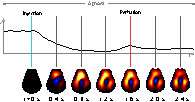
\includegraphics[width=0.8\textwidth]{chapter_2/imgs/fig-methodsBolus.pdf}
\end{flushright}
\caption{\label{fig:methodsBolus}%
The method used to select the perfusion point from the bolus injection is shown 
in the figure above. The point with the widest spread of high conductivity was 
selected as the point of perfusion, shown here at 1.6 seconds after the contrast 
agent injection. The image series shows the conductivity contrast as the bolus 
injection travels through the thorax.
}
\end{figure}


\subsubsection{Frequency-Filtering} \label{freqVent}

Heart-frequency EIT images during the selected events were calculated 
by taking the FFT of the time-series image data after first applying a Blackman window: 
$w(n)=a_{0}-a_{1}\cos \left({\frac {2\pi n}{N-1}}\right)+a_{2}\cos \left({\frac {4\pi n}{N-1}}\right)$ 
with $a_{0} = 0.42$, $a_{1} = 0.5$ and $a_{2} = 0.08$, where N is the number of time-series 
EIT images in the selected event.

An FFT was calculated from a series of images restricted to pixels in the heart 
region. From the FFT 
of all pixels the heart region, the heart frequency was selected as the largest 
peak between 3 and 4.5 Hz, representing a heart rate between 180 
and 240 bpm (typical for a newborn lamb).

The identified heart rate was used to select changes at the heart-frequency 
in the frequency domain images of the entire thorax. 
Images at 3 frequencies on either side of the heart rate were also reconstructed 
to account for changed in heart rate over the course of the data collection.
A Blackman window with a length of 7 was applied 
surrounding the heart frequency to generate a weighted mean of the images, resulting in 
a single perfusion image from the heart-frequency data. 
 
The output of the frequency filtering method is an 
image with complex values assigned to each pixel.  

Depending on the timing of the pulsatility-based changes within the selected signal
the real component of frequency analysed image 
did not correspond to the maximum conductivity 
change in the lungs in every event.
In order to correct this, each image was displayed along the axis that gave the maximum real component contained
within the lung region to ensure
the maximum change in impedance related to pulsatile activity in the lungs was calculated.

\begin{figure}
\begin{flushright}
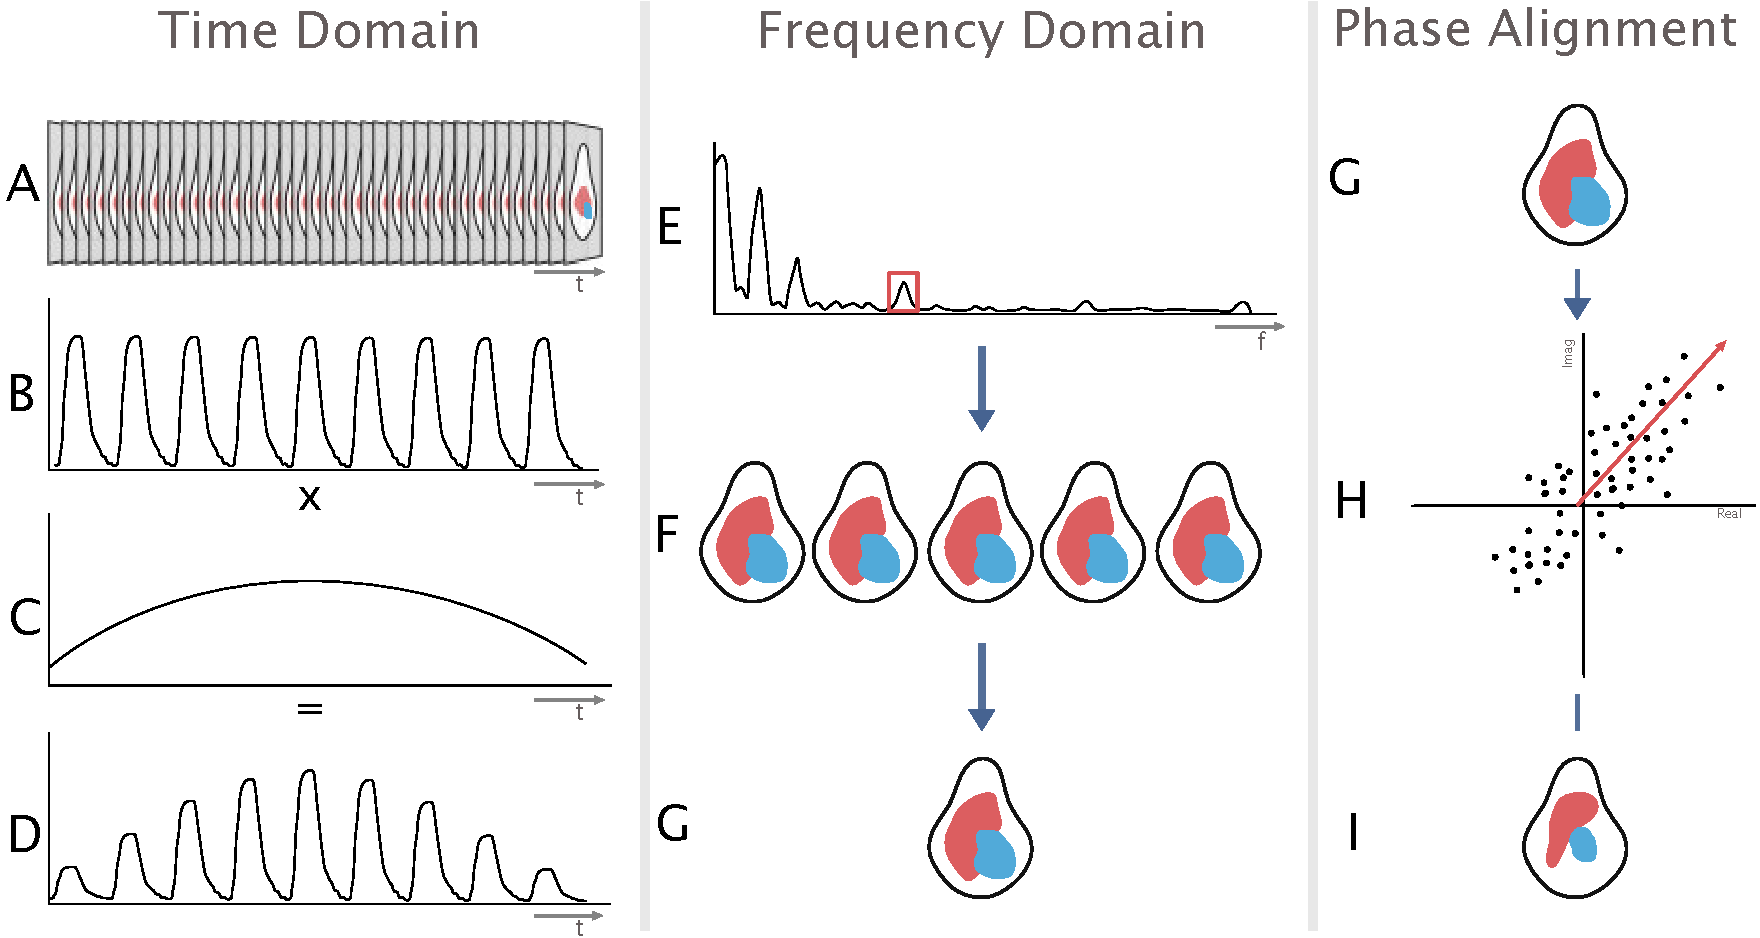
\includegraphics[width=0.8\textwidth]{chapter_2/imgs/fig-methodsFrequency.pdf}
\end{flushright}
\caption{\label{fig:freqAnalysis}
Frequency analysis methodology used for obtaining a perfusion image 
from the time series data. Steps are: 
A) to reconstruct the images from time series measurements; 
B) - D) window the time series data before performing a 
FFT on the data for each element; 
E) Select the dominant frequency between 3 and 4.5 Hz as the heart frequency;
F) reconstruct the image at the heart frequency and selected nearby frequencies; 
G) take the mean of the images at the heart frequency using a Blackman window 
to give greater weight to those closer to the center; 
H) I) select the image that will give the maximum real component contained
in the lung region.
}
\end{figure}

\subsubsection{Ensemble Averaging}

Time series data of the total impedance signal for each pixel in the heart region was filtered 
using a bandpass filter to eliminate noise and breathing changes, 
and allow the heartbeat to be seen clearly in the signal.
Peak detection was used on this heart-region data
to select the amplitude peaks in impedance change
signal at the heart frequency.

Using the identified time points, the global impedance change signal 
was ensemble averaged by overlaying all identified peaks 
to give an averaged heartbeat. 13 images were reconstructed over the 
course of the heart beat to select the image that resulted in the maximum 
positive increase impedance within the lung region. This process is outlined 
in~\fref{fig:timeAnalysis}.

\begin{figure}
\begin{flushright}
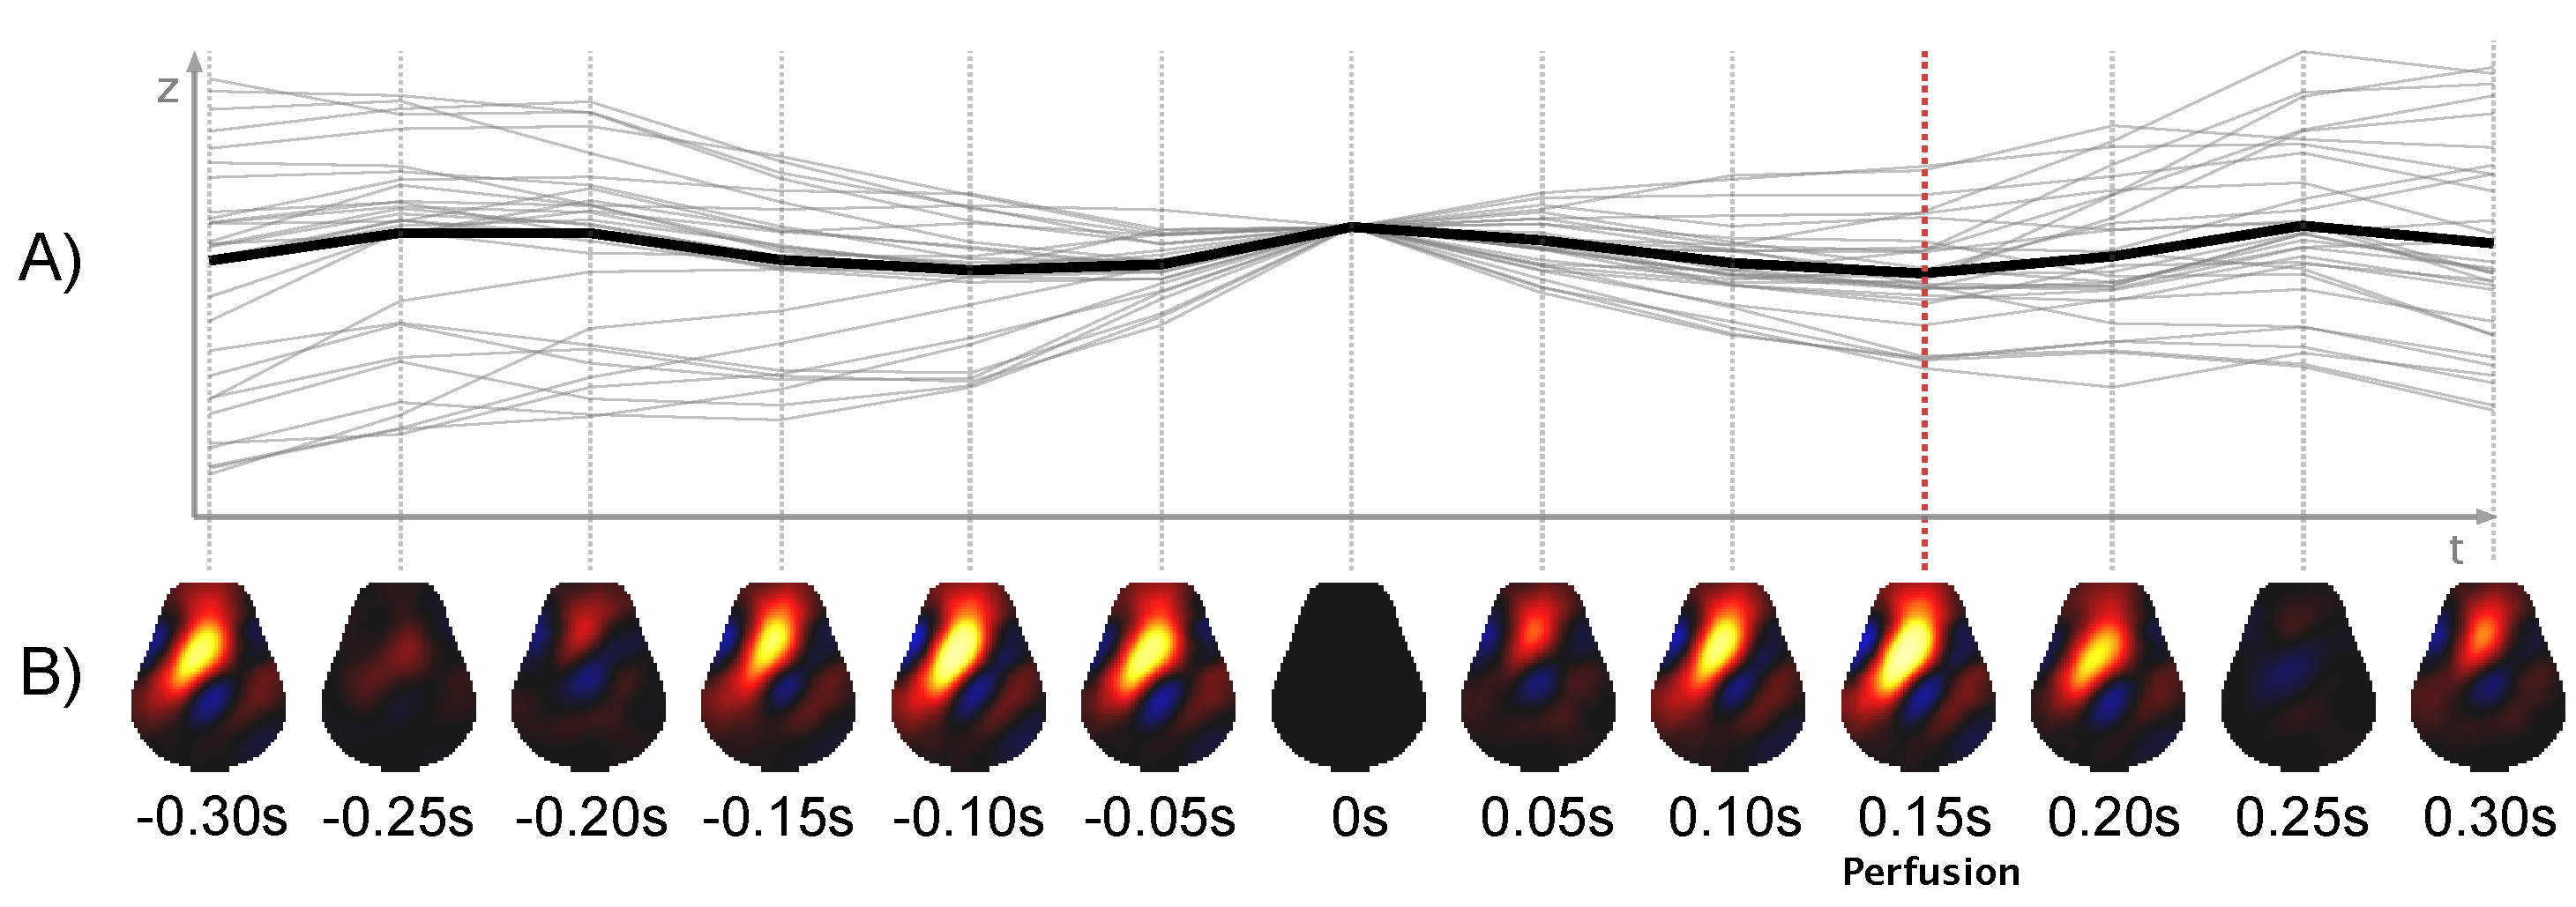
\includegraphics[width=0.8\textwidth]{chapter_2/imgs/fig-methodsTime.pdf}
\end{flushright}
\caption{\label{fig:timeAnalysis}%
Illustration of the stages of the ensemble averaging process:
A) an ensemble average of all heartbeats over the time frame is taken from the 
summed global signal; and 
B) shows reconstructed images corresponding to each time point 
in the global ensemble averaged signal above.
The selected perfusion image is the image with the maximum impedance increase in the 
lung region.
}

\end{figure}

\subsection{Image Comparison}

To compare the images the Jaccard 
distance between functional EIT images was calculated. 
Negative impedance changes were removed from the images
and the images were normalized.

The Jaccard distance was calculated between the reference image 
calculated using the maximum increase in lung-region conductivity during 
bolus injection (b), and the frequency-based method (f):
$J(x,y) = \sum_{i}\frac{min(b_i,f_i)}{max(b_i,f_i)}$
representing the distance between the two images.

\subsection{Statistical Analysis}

To determine the significance of the change in bolus between postures
and methods, the Cohen's d score was calculated to quantify the effect size of
the change in the centre of mass of the perfusion image~\parencite{Cohen1988}.  
This was calculated as the difference between two means over the pooled standard deviation. 
Where the difference between the two means is: $\mu_1-\mu_2$, and the pooled
standard deviation is: ${\sqrt{\frac{(n_1-1)s^2_1+(n_2-1)n_2s^2_1}{n_1+n_2-2}}}$. 

\section{Results}                         %% RESULTS %%

The Jaccard scores for each method were compared between 
ensemble averaging and frequency filtering methods to determine the regions where performance 
was best for each method. Figure \ref{fig:resultsJaccard} shows a 
comparison between Jaccard distance for each animal, connecting lines 
indicate different methods performed on the same data segment, while each marker shape
denotes a separate posture.

\begin{figure}
\begin{flushright}
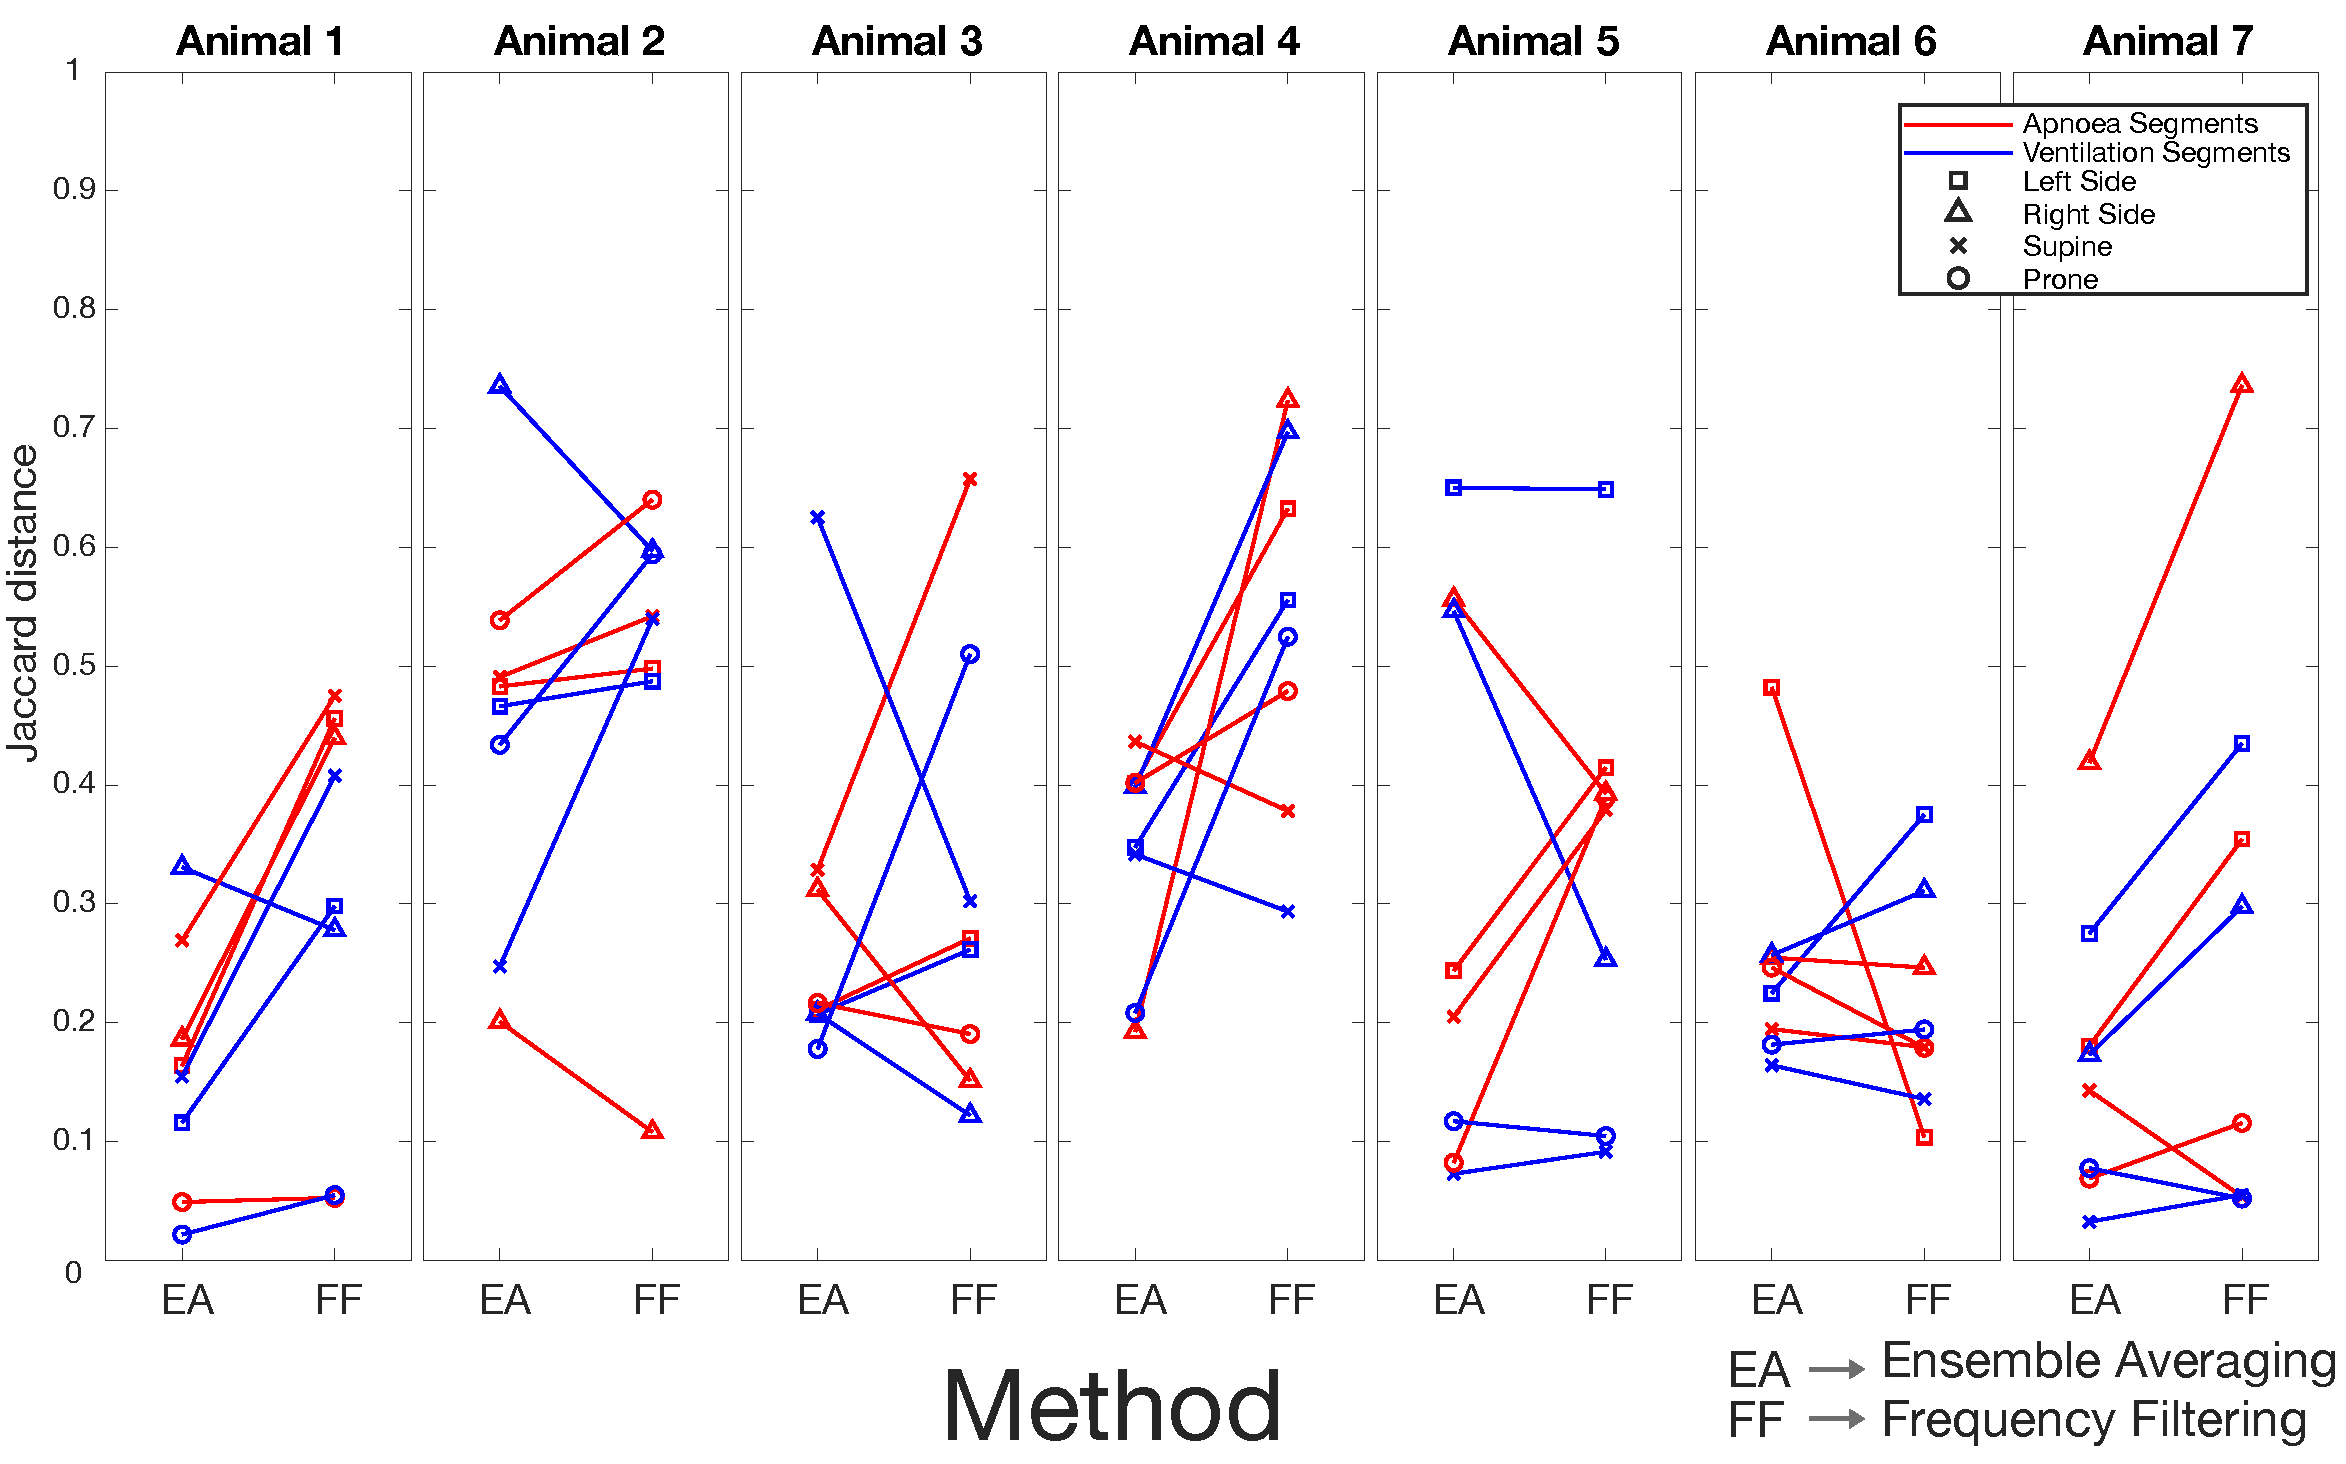
\includegraphics[width=0.8\textwidth]{chapter_2/imgs/fig-resultsJaccard.pdf}
\end{flushright}
\caption{\label{fig:resultsJaccard}%
Jaccard scores for each method and animal in the comparison. Frequency 
filtering and ensemble averaging methods performed on the same data segment are 
connected by solid lines. Red lines and markers indicate apnoea data sections, 
while blue indicates ventilation data sections. Each posture is denoted by a different
shaped marker in the figure.
}
\end{figure}

On average frequency filtering outperforms ensemble averaging based methods
of perfusion calculation (p=0.04), and there is no significant difference in
performance of the heart-frequency based 
filtering techniques during periods of apnoea relative to periods of ventilation.

Of the 56 data regions that were analysed,
the ensemble averaging performed better in 12 cases and the frequency 
filtering achieved the best performance in 28 cases, there, were 16 additional cases 
where the difference in performance was negligible at less than 5\%. On 
average, across all images, frequency filtering based methods scored
7\% higher than ensemble averaging.

The center of mass of the perfusion 
measure images using the bolus injection method had a Cohen's d score of less than 0.1 
between posture changes
indicating that there is an insignificant or trivial difference in the means relative
to the standard deviation \parencite{Cohen1988}. 
To demonstrate the visually observable changes due to posture change and the 
high similarities that can be observed between filtering- and bolus-based 
perfusion estimates, frequency filtered images from 
animal 4 are compared to bolus based methods in \fref{fig:discussionSample}.

\begin{figure}
\begin{flushright}
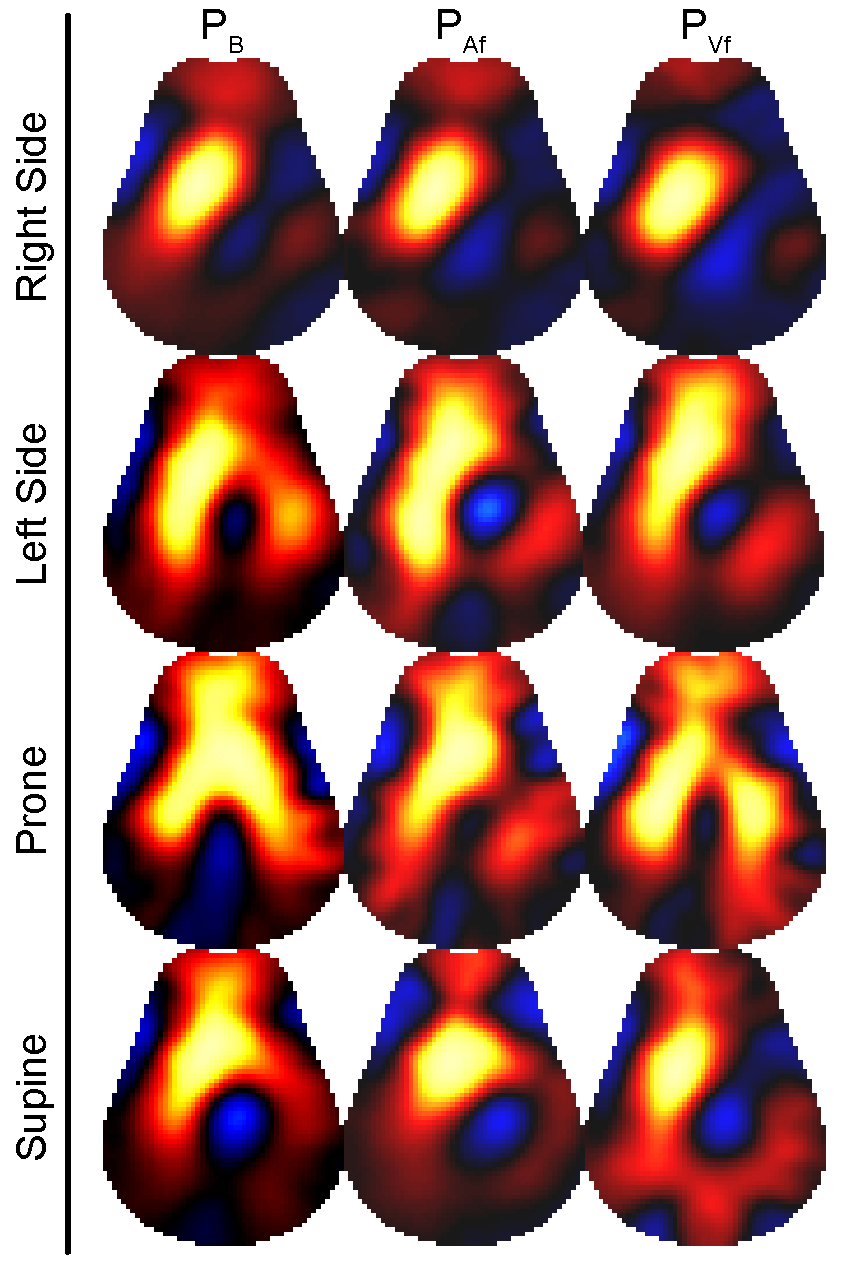
\includegraphics[width=0.7\textwidth]{chapter_2/imgs/fig-discussionSample.pdf}
\end{flushright}
\caption{\label{fig:discussionSample}%
		This figure shows the tracking of perfusion for frequency filtering measures
		of perfusion during apnoea and ventilation sections compared to bolus injection
		for animal 4.
$\PBi$ is the bolus injection image, 
$\PAi$ uses the frequency filtering method during apnoea and
$\PVi$ is the frequency filtering method during ventilation.
}
\end{figure}

\section{Discussion}                             %% DISCUSSION %%

Two primary approaches of EIT perfusion calculation
have been compared in this paper: injection
of a bolus of contrast-agent resulting 
in EIT image changes which produce perfusion measures, and
digital filtering of EIT image sequences to extract
the heart-frequency components.
Additionally, various algorithms have been evaluated
for digital filtering-base approaches during mechanical 
ventilation and short apnoea sequences, 
using both frequency- and ensemble averaging-based techniques.
There have been few comparisons of
these techniques, and 
we set out to better understand the relationship between
perfusion and heart-frequency measures, and between the various filtering
approaches used to determine heart-frequency cardiac changes.
We selected an experimental protocol using posture-change 
to alter the regional distribution of lung ventilation
and perfusion in newborn lambs.

Our first question was
``to what extent do heart-frequency filtering-based measures correspond to perfusion?''

The primary results (\fref{fig:resultsJaccard}) use a Jaccard index of the similarity
between functional images. Overall it was found that in healthy animals 
the Jaccard index indicated good agreement with our gold standard. While highly
dependant on the data, it was found that there was a high degree of similarity 
between methods with respect to
the overall shape of the perfusion. 
In both animals 2 and 4, where the signal required little preprocessing before analysis 
there is a higher Jaccard score across all cases.

The synchronisation box was attached to the EIT system but was not used for this experiment,
an error in the connection caused brief periods of the signal (less than 1\,s) in some animals to be zeroed.
Through careful processing of this signal only brief sections of data were lost and we do not feel this
impacts the results.

% Limitations
During the experiment the order of posture change was not randomised. 
While changes in ventilation due to posture change
are not understood to have long term physiological effects, if there is a longer term
effect of change in posture the lack of randomisation will impact the results. 
\citeauthorandyear{Nguyen2015} were able to image perfusion changes due to induced 
pulmonary embolisms and using the peak impedance change on dilution curves,
however our data presented insufficient variance in perfusion induced by posture change to 
complete a center of mass analysis. A higher statistical power 
could potentially be achieved through initiating posture changes
with more dramatic results in perfusion, such as upright to supine \parencite{Nakazato2010}.

Throughout the experiment, 
the perfusion image was selected as the image containing 
the largest increase in conductivity in the sum of pixels 
in the lung region, which occurred 
at different relative times across animals and events. Many factors could affect this
including belt positioning changes, and it could be a contributing factor 
to the inconsistent trends in amplitude changes in the global image across methods.
\citeauthorandyear{Borges2012}
compared EIT perfusion images using first-pass kinetics and 
heart-frequency filtering based methods to perfusion measures using SPECT,
finding that heart-frequency filtering
techniques made systemic errors when used to estimate the perfusion. They also 
determined that there was no discernible relationship between the magnitude of the
SPECT images and the heart-frequency images.
This was consistent with the findings of this study that image amplitude of the bolus injection and 
heart-frequency filtering-based methods was not consistent in all animals.
This methodology presented by \citeauthorandyear{Borges2012}
was not part of the comparison in this study as the edentification of the 
perfusion signal due to the heart could not be consistently
identified and removed across all animals.
In two dimensions, heart-frequency and ventilation signals 
have been used to identify the location 
of the heart and lungs within the EIT electrode plane with known electrode 
locations and anatomy~\parencite{Ferrario2012}, but in situations where the electrode 
location and anatomy is not precisely known EIT tends to perform poorly as a structural 
imaging modality~\parencite{Adler2017a}.
These challenges suggest that configurations with multiple planes of electrodes 
may be better able to isolate and remove off-plane 
pulsatility signals related to the heart.

It was observed that the general shape of 
the perfusion was consistent across all methods despite amplitude variations. 
One reason for the difference in amplitude change across animals may be due 
to slight variations in the belt placement and electrode positioning on the animals.
If the belt is closer to the heart, there will be a larger heart-frequency component 
to the signal and there may be a variance in the impedance change due to bolus injection.

Next, we asked ``what are the advantages and disadvantages of different approaches
to heart-frequency filtering of EIT data, and which techniques are recommended
under which circumstances?''

Our overall recommendation is that, whenever possible, 
frequency filtering techniques should be used. This is largely
because frequency filtering methods tend to be more stable in the 
presence of noise on the signal. 
Ensemble techniques are advantageous
in some circumstances, because they better use the heart-frequency
variability to avoid interference from harmonics of the
ventilation at the heart rate. For frequency-filtering
techniques, it is necessary to widen the heart-frequency
filters to account for such variability.
On the other hand, it is sometimes not possible to accurately
synchronize heartbeats, due to noise corruption in the
signals or the very low amplitude of the heart-frequency signals
relative to the ventilation signal.
In cases where the signal of the heartbeat 
was not clearly identifiable through visual inspection of the signal, neither 
ensemble averaging nor frequency filtering was able to achieve good 
estimates of perfusion relative to the bolus injection event. 

In summary, 
our goal was to understand the relationship between bolus- and filtering-based
EIT measurements of lung perfusion, as well as the relationship between different
filtering-based measures of perfusion.
Our results indicate there is a common trend between the shape and perfusion  
estimates of both heart-frequency and bolus injection images 
despite the difference in physiological events behind each measure.
Amongst filtering techniques, frequency
filtering outperforms ensemble averaging across regions of data where there is noise present and the 
heart signal cannot be readily identified, and both methods were able to approximate the bolus injection 
measures equally well when applied to apnoea and ventilation regions of data.

\chapter{FEM mesh refinement for 3D Electrical Impedance Tomography}

%\begin{abstract}
\section{Summary}
In this paper we examine the requirement for mesh refinement around 
electrodes in Electrical Impedance Tomography (EIT). 
While it has been recommended that  models be refined around the electrodes, where current
density and sensitivity are highest,  the level of refinement required is poorly understood. 
Using a set number of nodes, we investigate the optimal distribution 
between the electrodes and 
the volume of a model. 
A balance point is used to measure the difference in distribution between the electrode and the centre of
the model.
To calculate this, all nodes contained between the surface of a selected electrode and the centre of the model 
were identified and the mean position of nodes along the container axis was computed. 
%A balance point was defined as the mean distance of all nodes along the axis 
%of a container encompassing all points between the centre of the model and the surface of a selected electrode.
We compare refinement strategies across commonly used meshing software in EIT and compare the 
model sensitivity error to an ultra-fine reference mesh. 
In a tank model, for a fixed number of nodes, error in the sensitivity calculation is minimized 
when the balance point of the nodes is n  85\% of the tank radius and the node density dissipates evenly 
from the electrode surface to the centre of the model. Using this method sensitivity error was decreased 
in all regions with high sensitivity. This node distribution technique  enables the generation  of accurate 
meshes with fewer nodes that can reduce measurement error and computing time. 
%\end{abstract}

\section{Introduction}
Electrical Impedance Tomography (EIT) reconstructs images of 
electrical tissue properties within a body from electrical
transfer impedance measurements at surface electrodes. For
biomedical imaging applications, it is being actively studied
for monitoring
the movement of air and blood in the thorax, and for imaging
the head and breast. Reconstruction of EIT images requires
the solution of an inverse problem in soft field tomography.
EIT image reconstruction requires 
calculation of a sensitivity matrix, $\bf J$, representing the relationship between internal changes and measurements
 . A pseudo-inverse of $\bf J$ is used
to update the image estimate over several iterations. 
EIT image reconstruction is ill-posed, since the physics of
current propagation implies that sensitivity is largest near
the electrodes and smallest in the body centre.

It is therefore clear that a precise  calculation of $\bf J$ is
required for solution accuracy. Since it is generally not
possible to use analytic solutions, because of the non-regular
shapes of biological bodies and the boundary conditions on a
conductive electrode, the finite element method (FEM) is typically
used. 
One key advantage of the FEM is that element size can be
selectively refined in regions to meet solution accuracy. 
The accuracy of the FEM solution will increase as more elements are
added, so a high mesh density is often desired to achieve an 
accurate solution. 
In this paper we will use the term mesh to refer to a specific 
combination of nodes and elements in a finite element model. 
In EIT the sensitivity is nonuniform 
across the entire model.
Thus
it has generally been recommended in the EIT literature 
that meshes be refined near electrodes, where the electric 
field and sensitivity are largest~\parencite{adler_electrical_2017}. 
This recommendation gives rise to two questions: 
1) No thorough analysis has been made to determine how much 
refinement is required. Given a ``mesh element budget'', what should
balance of nodes be between the centre of the model and the electrodes? And 
2) How do different freely available meshing tools that are
commonly used with EIT compare when used to refine 3D meshes?

Previously with EIT, mesh refinement has primarily been either 
constant, or based on 
the complexity of geometric surfaces and lines within a model~\parencite{grychtol_fem_2013}.  
In EIDORS~\parencite{adler_uses_2006} meshes are generated using both 
Netgen~\parencite{schoberl_netgen_1997} and Gmsh~\parencite{geuzaine_gmsh_2009} 
for 2D and 3D models. 
Refinement around electrodes is commonly performed by 
setting a mesh density for the electrodes and allowing the mesh density to 
decay towards the maximum mesh size. This does not allow the user to specify 
the rate of decay or precisely control the mesh size.   

A model that accurately represents the anatomy of the imaged region 
can greatly increase the quality of the reconstructed image~\parencite{grychtol_impact_2012},
but increasing the complexity of mesh surfaces presents additional challenges for
mesh refinement.  EIT reconstruction software EIDORS enables users to place electrodes on the surface of complex 
boundaries~\parencite{grychtol_fem_2013}, but the current functionality does not  
enable control of the refinement around the electrodes or internal 
structures.
Most commercially available FEM packages
do not conveniently provide such capability either.

%Due to the increasing number of options for implementing mesh refinement around the
%electrodes it is also important to consider which gives the highest quality mesh. 
%The quality of a mesh dictates the accuracy of the subsequent analysis 
%and solution, and can be characterized by the properties of the tetrahedra
%comprising the model~\parencite{Parthasarathy1993}.
In this paper we investigate approaches to manage the tradeoff
between refinement of the electrode regions versus the bulk volume. 
We present a comparison between Gmsh and 
Netgen based mesh refinement around electrodes, and evaluate the 
effect of mesh refinement techniques on error in  the sensitivity matrix, 
$\bf J$. 

\section{METHODS}
\subsection{Overview}

We built a cylindrical model in Gmsh and Netgen which was parameterized so that multiple
different combinations of mesh refinement were possible.
These results were compared to a very high density meshes which was considered the gold standard.
% TODO ADD THE FOLLOWING IN THE INTRO

\subsection{Mesh Generation}
A cylinder ($\diameter=0.5$~m, height $h=0.25$~m) with four square electrodes 
(5~cm edge length) placed equidistantly around the perimeter at mid-height was
meshed with Netgen (version 5.3.1)~\parencite{schoberl_netgen_1997} and Gmsh 
(version 4.7.0)~\parencite{geuzaine_gmsh_2009}
meshing software.
Current was injected between adjacent electrodes and the voltage was measured between the remaining
two electrodes.
For 3D meshes an initial analysis was done building on work from 
Grychtol and Adler~\parencite{grychtol_fem_2013} where mesh density was
set by specifying the maximum edge lengths permitted on electrode surfaces
and in the volume of the FEM.
Results were compared against those generated using ultra-fine meshes. 
Calculations were performed with EIDORS (version 3.10)~\parencite{adler_uses_2006} 
in Matlab 2019b
(The Mathworks, Natick, MA, USA).


Meshes of different sizes were generated with Netgen and Gmsh by manipulating the desired
maximum edge length (maxh parameter) for the entire domain and the electrodes.
Two  mesh analyses were performed. For the first
mesh maximum element lengths were
chosen such as to divide the electrode side of 5~cm into an integer number of
segments of equal size. 
The maximum mesh element length ranged from 1 to 7 subdivisions of the electrode 
edge, while the maximum mesh element length in the ultra-fine reference mesh  
was 15 subdivisions per 
electrode edge. Independent reference meshes were generated for each software.
Two types of models were generated this way. Constant models C1--C7, where the mesh size 
was constant, and refined models R1--R7 where the electrode mesh size was specified and 
dissipated towards an internal mesh element size of 5 cm. Additional refined meshes were
generated with reduced mesh size in the internal mesh regions.  
R1-R7 is referred to as refinement A where the internal element max size was 5 cm. Refinement 
B had an internal mesh size of 4 cm, C was 3 cm and D was 2 cm.
The numeric value in the mesh 
ID indicated the number of subdivisions per electrode edge. 
In Netgen the mesh decay was not controllable, but in Gmsh the size was set 
to increase evenly from the surface of the electrode to the centre of the model.
\fref{fig:sample_meshes} shows example meshes of coarse, fine and refined
meshes. \fref{fig:electrode_mesh_size} shows the generated mesh structure for 
constant refinement meshes around the electrode 
for both Netgen and Gmsh. 


\begin{figure}
   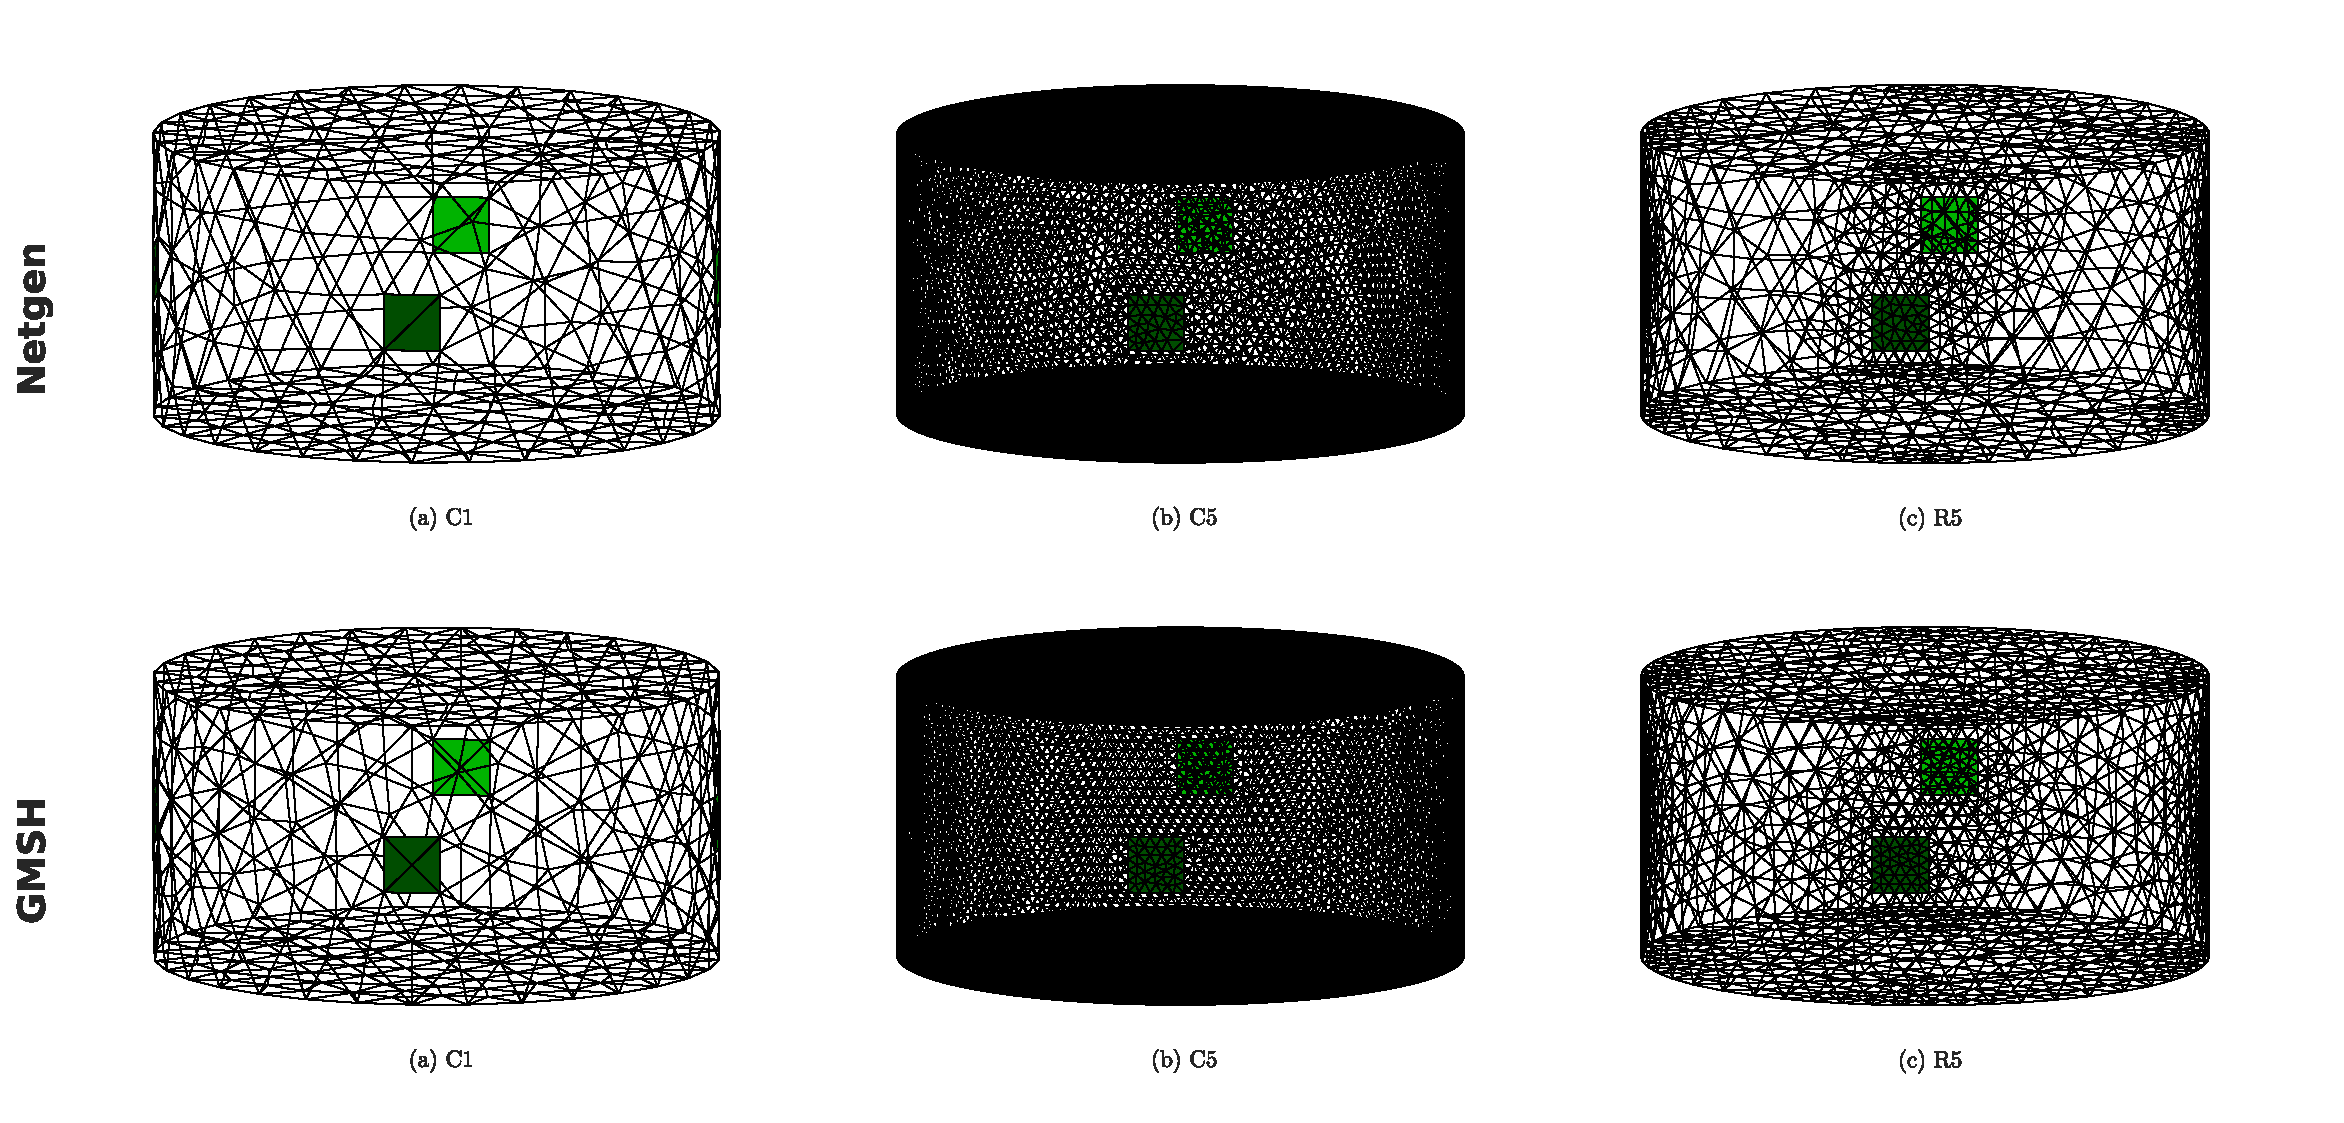
\includegraphics[width=\columnwidth]{chapter_3/imgs/sample_meshes.pdf}
   \caption[Example meshes for various refinement strategies]{\label{fig:sample_meshes} 
   Sample meshes generated with Netgen (top row)
   and Gmsh (bottom row). From left to right: (C1) the coarsest constant
   mesh; (C5) a refined constant mesh; and (R5) a refined mesh with the same
   electrode mesh density as C5 but lower internal mesh density.}
\end{figure}

\begin{figure}
  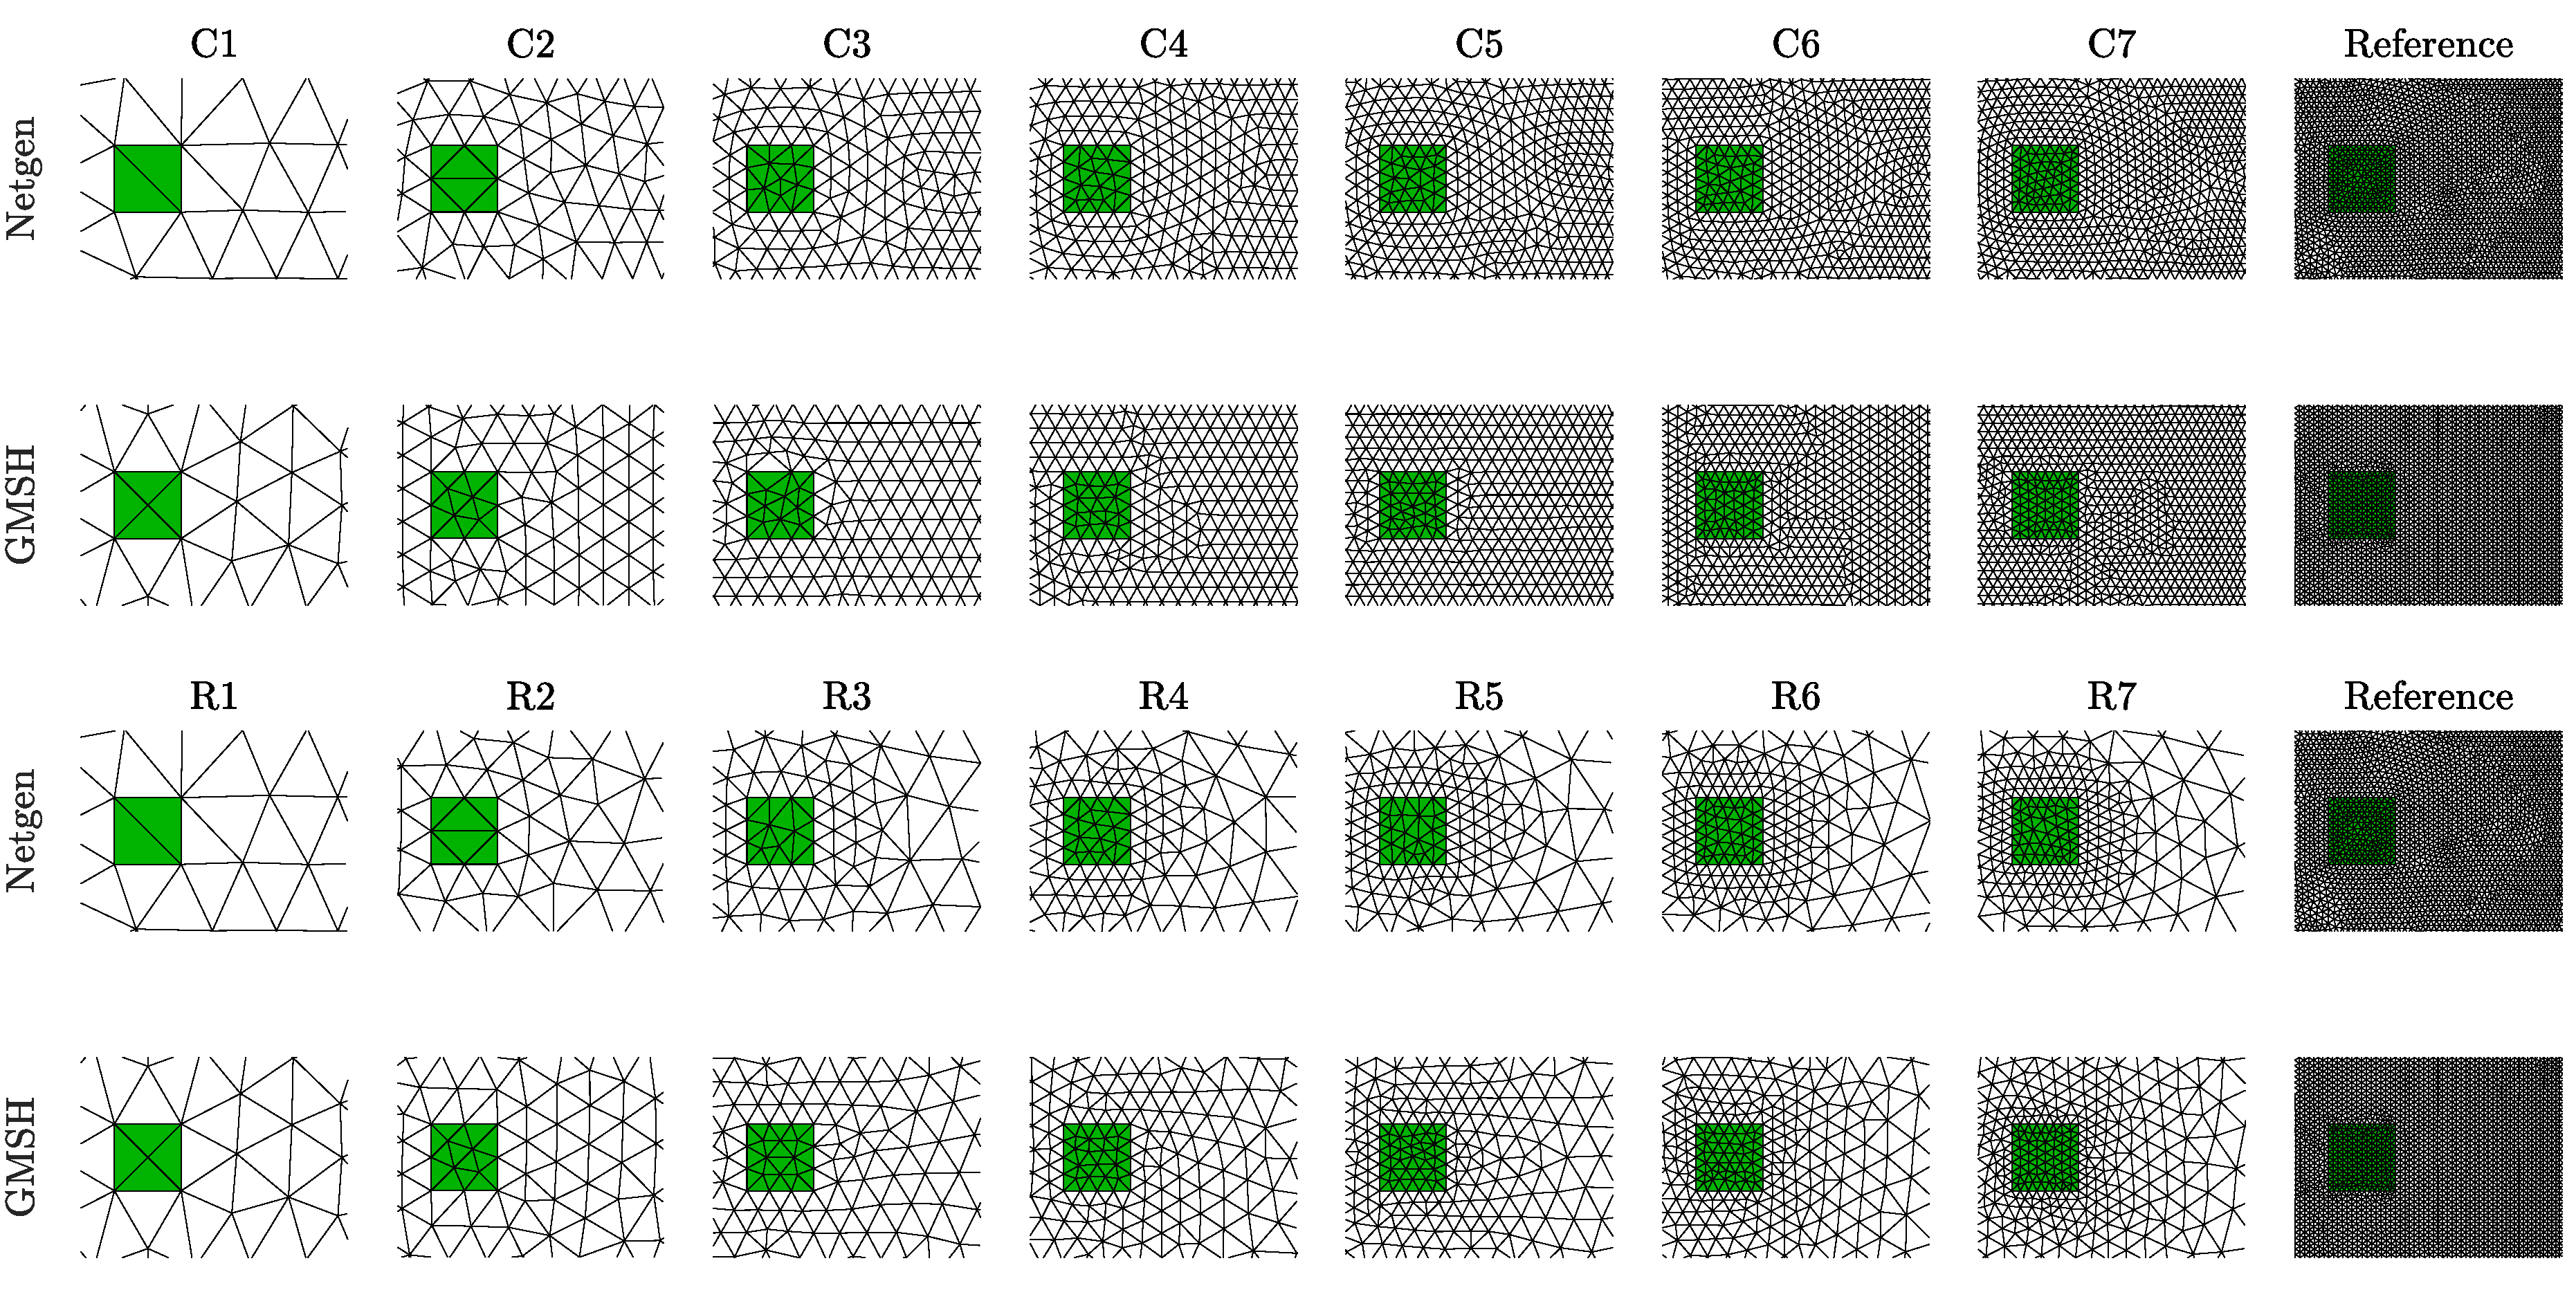
\includegraphics[width=\textwidth]{chapter_3/imgs/electrode_mesh_size_large.pdf}
  \caption[Mesh size surrounding the electrode]{\label{fig:electrode_mesh_size} A view of the electrode meshing for all constant-density meshes 
  in Netgen and Gmsh. The top two rows show all electrode faces and immediate surrounding
  surroundings from coarsest (C1) to finest (C7). C represents the constant mesh refinement and the number
  represents the specified mesh subdivisions per electrode edge. The reference mesh is equivalent to C15.
  The bottom two rows show refined meshes R1 to R7 with both Netgen and Gmsh and shows the rate of mesh
  dissipation away from the electrodes.}
\end{figure}

For the second analysis, the distribution of nodes within the 
model was changed without altering 
the total number of nodes to give M1 -- M17. 
Starting with the constant mesh C3 as M1, the maximum mesh element 
length on the electrode was decreased by 10\% and the maximum mesh size in the centre was
increased so that the total number of elements in the mesh was  within 10\% of the 
original mesh. C3 was chosen as the starting point because several steps of mesh 
refinement could be generated before the electrode mesh density surpassed the reference meshes. 
For mesh M17 the specified electrode refinement was equal to the reference mesh. 
In Netgen the mesh dissipation rate was not further controlled, and in Gmsh the mesh density 
decreased evenly from the electrode surface to the centre of the model. 
To compare these meshes a section of the model was selected
encompassing all points between the centre of the model and a selected electrode face.
The average 
distance, or balance point, along the x-axis of the selected points was expressed 
as a percentage of the tank radius.
This process is illustrated in \fref{fig:balanceMethods}.
 
\begin{figure}
  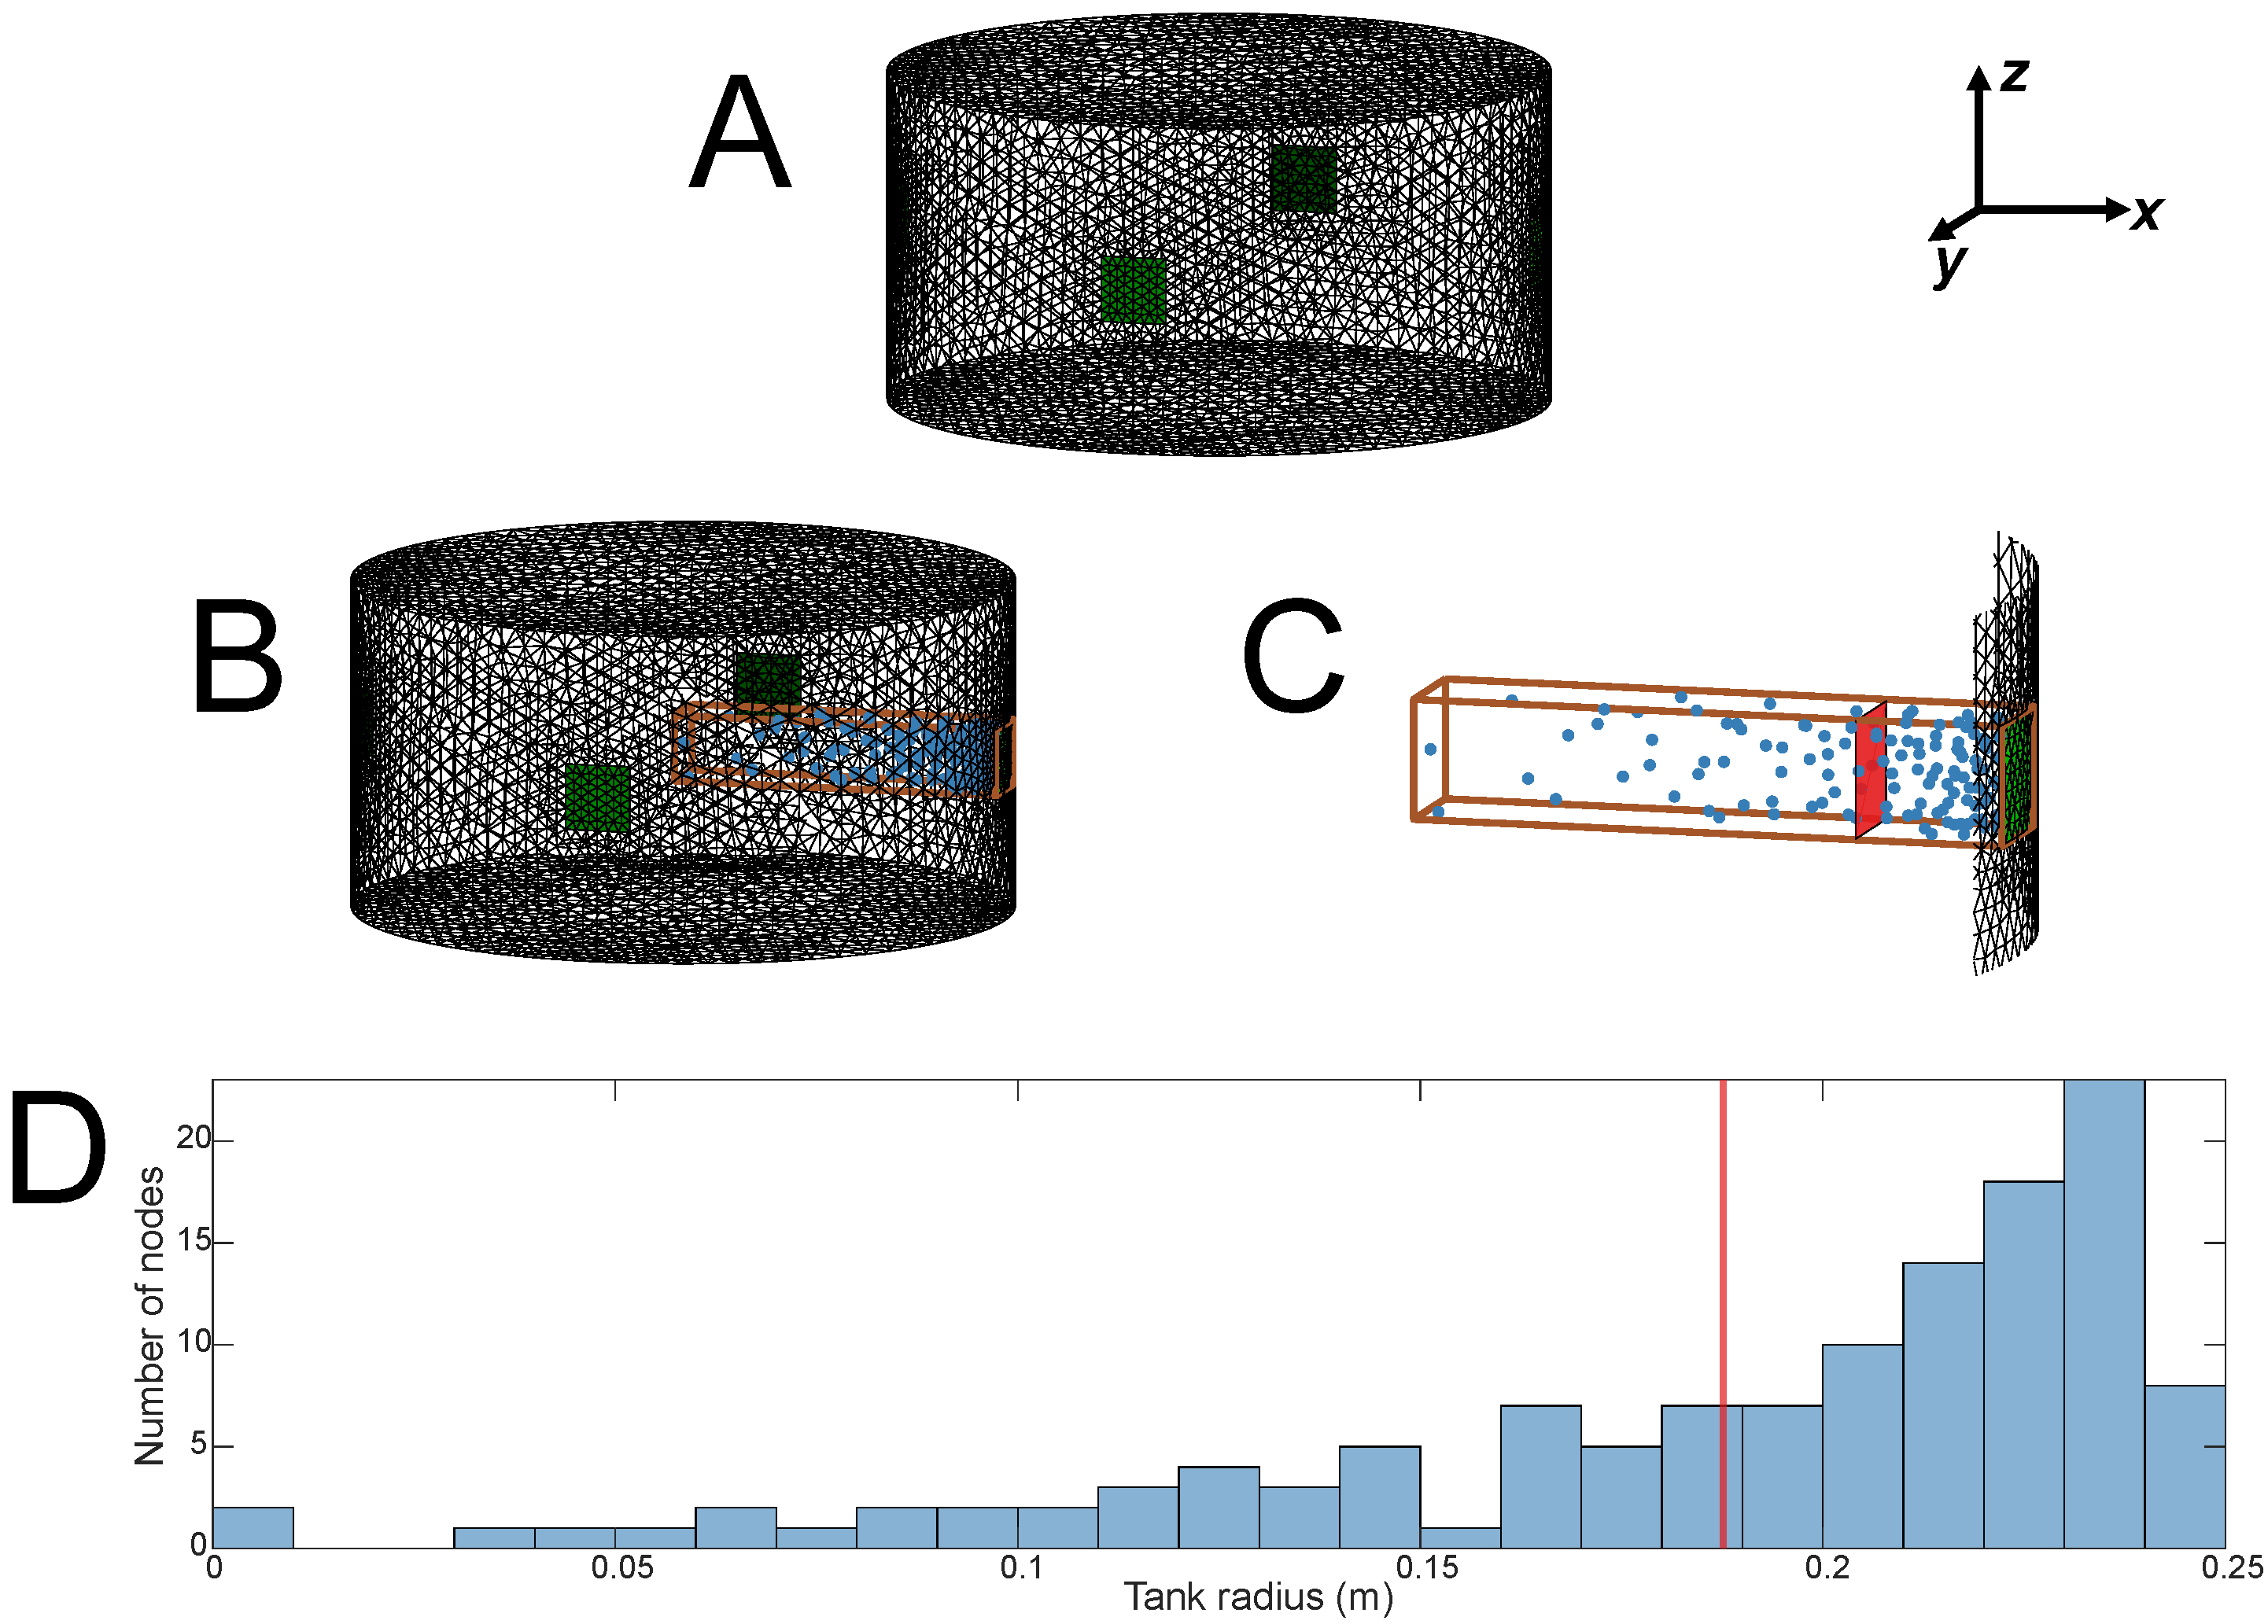
\includegraphics[width=\columnwidth]{chapter_3/imgs/balance_methods.pdf}
  \caption[Balance point calculation method]{\label{fig:balanceMethods} A sketch of the process to determine the 
  balance point of generated meshes. A) the starting mesh; B) nodes between the
  electrode surface and the centre of the model are identified; C) the 
  balance point of the nodes along the x-axis is calculated and indicated 
  by the red plane; D) a histogram showing an example distribution and balance point (red)
  for the selected model.}
\end{figure}

When generating meshes to compare across several mesh density profiles as the balance of the nodes was shifted 
towards the electrodes, 19 meshes were generated for each software including 2 reference meshes. 
\fref{tab:mesh-table} shows the parameters of the resulting odd numbered meshes. 

% Table 
\begin{table}[]
\caption[Parameters used to generate meshes]{\label{tab:mesh-table}Mesh parameters for odd numbered meshes generated by Netgen (A) and Gmsh (B) 
to determine the optimal 
node balance. Parameters global maxh and electrode maxh refer to the specified input parameters; the remaining 
columns give parameters from the resulting meshes.}
\begin{tabular}{p{0.7cm}p{0.2cm}p{1cm}p{1cm}|p{1.4cm}p{1.4cm}p{1cm}|p{1.3cm}p{1.3cm}p{1.3cm}p{1.3cm}}
\multicolumn{2}{l}{Mesh ID} & glbl. maxh [mm] & elec. maxh [mm] & \#~elem. & \#~nodes & \#~elec. elem. & minEL\textsuperscript{\emph{a}} [mm] & maxEL\textsuperscript{\emph{b}} [mm] & minEV\textsuperscript{\emph{c}} [mm\textsuperscript{3}] & maxEV\textsuperscript{\emph{d}} [mm\textsuperscript{3}]\\ \hline 
\multirow{2}{*}{M-01} &A & 16.67 & 16.67 & 31347 & 7095 & 22 & 9.80 & 49.45 & 254.76 & 6851.01\\ 
& B & 16.67 & 16.67 & 49210 & 9615 & 25 & 10.32 & 50.00 & 222.87 & 2898.59\\ 
\multirow{2}{*}{M-03} &A & 18.33 & 15.00 & 29639 & 6482 & 22 & 10.75 & 50.41 & 289.80 & 5826.14\\ 
& B & 18.33 & 15.00 & 49247 & 9680 & 40 & 7.36 & 37.11 & 172.78 & 2814.55\\ 
\multirow{2}{*}{M-05} &A & 18.33 & 13.33 & 29814 & 6589 & 28 & 9.39 & 49.91 & 162.26 & 5648.41\\ 
& B & 20.00 & 13.33 & 50749 & 9930 & 42 & 7.80 & 37.93 & 134.41 & 3233.59\\ 
\multirow{2}{*}{M-07} &A & 18.33 & 11.67 & 30581 & 6723 & 36 & 8.77 & 47.88 & 141.74 & 6252.36\\ 
& B & 21.67 & 11.67 & 53002 & 10429 & 60 & 6.17 & 40.84 & 63.22 & 4077.18\\ 
\multirow{2}{*}{M-09} &A & 18.33 & 10.00 & 30690 & 6755 & 42 & 7.86 & 49.18 & 115.45 & 5496.39\\ 
& B & 23.33 & 10.00 & 56237 & 11008 & 68 & 5.82 & 43.81 & 62.88 & 4962.89\\ 
\multirow{2}{*}{M-11} &A & 18.33 & 8.33 & 31575 & 7030 & 74 & 6.05 & 50.99 & 60.06 & 6086.88\\ 
& B & 26.67 & 8.33 & 55545 & 10886 & 96 & 5.51 & 49.72 & 36.84 & 7424.70\\ 
\multirow{2}{*}{M-13} &A & 20.00 & 6.67 & 28589 & 6447 & 92 & 4.65 & 51.85 & 20.68 & 6664.11\\ 
& B & 30.83 & 6.67 & 54993 & 10825 & 148 & 4.51 & 55.36 & 20.63 & 10453.90\\ 
\multirow{2}{*}{M-15} &A & 21.67 & 5.00 & 27775 & 6245 & 158 & 3.46 & 52.60 & 11.13 & 9097.30\\ 
& B & 36.67 & 5.00 & 55331 & 11000 & 250 & 3.51 & 61.66 & 7.99 & 15838.09\\ 
\multirow{2}{*}{M-17} &A & 30.00 & 3.33 & 39116 & 7590 & 320 & 1.75 & 72.83 & 1.13 & 23783.17\\ 
& B & 48.33 & 3.33 & 52947 & 10798 & 548 & 2.32 & 86.60 & 2.72 & 32287.34\\ \hline 
\multirow{2}{*}{REF} &A & 3.33 & 3.33 & 6661789 & 1173243 & 510 & 1.75 & 9.49 & 1.01 & 46.09\\ 
& B & 3.33 & 3.33 & 5871464 & 976558 & 554 & 2.10 & 7.59 & 1.58 & 21.65\\ 
\multicolumn{11}{c}{\emph{a}: minimum mesh edge length, \emph{b}: maximum mesh edge length}\\ 
\multicolumn{11}{c}{\emph{c}: minimum mesh element volume, \emph{d}: maximum mesh element volume}\\ 
\end{tabular}

\end{table}

%The difference in meshing algorithms meant that the meshes did not have the same number
%of elements, or elements per electrode for a given input. To compare meshing 
%algorithms the error and sensitivity were compared to the average number of mesh elements\
%across all electrodes. 
%
%
%%The settings used to generate all thirty meshes and their sizes are reported
%%in Table~\ref{tab:meshes}. 
%%{\COMMENT{Broke table with new analysis - need to re-insert after electrode mesh fix.}}
%
%The mesh quality was measured as a function of the minimum angle of the tetrahedra
%for the volumetric mesh, and the minimum angle of the triangles in the surface mesh.

\subsection{Simulation}
The potential at each node \VB\ of the mesh was calculated using the finite
element method (FEM) using the linearization 
\begin{equation}
\VB = \YB^{-1}\CB
\end{equation}
where \YB\ is the admittance matrix of the FEM (and a function of conductivity
distribution) and \CB\ is a matrix representing the current injection pattern,
such that \CB$_{ij}$ represents the current injected in electrode $i$ during
the $j$-th stimulation. Here, we drive current of 1~A between two adjacent
electrodes in a single stimulation, so $C = [0\,|\,0\,|\,1\,|\,-1]^T$. 
We pick a node in the centre of the FEM as ground, since it is necessary to
assume the potential on
one node for \YB\ to be invertible.
We use the complete electrode model and assume contact impedance of
0.01~$\Omega$ in the calculation of the admittance
matrix~\parencite{polydorides_electrode_2002}. 

%The resultant potential distribution in the
%electrode plane, calculated for the finest mesh and subsequently projected onto
%a $512\times512$ pixel grid, is presented in Fig.~\ref{fig:ref:a}.
%The potential distribution \VB\ is used to visualize the current flow
%around the measuring electrodes.
% NOT CURRENTLY LOOKING AT THE CURRENT FLOW! seems to be a repeat of the same stuff

We calculate the sensitivity (or Jacobian) matrix \JB\ of measurements \vB\ to
changes in the conductivity $\sigma$ of individual elements as
$\JB_{ij}=\frac{\partial v_j}{\partial \sigma_i}$ using the adjoint
method~\parencite{polydorides_electrode_2002}. Again, since we only have one measurement, \JB\
is in fact a vector.
We construct a sensitivity image by assigning each element
$i$ of the FEM the value of \JB$_i$ divided by the element's volume.
Mean sensitivity in the plane of electrodes is then calculated by averaging
the sensitivity in fifteen planes parallel to the plane of electrodes and
spanning the height of 5~cm. 
The sensitivity was projected onto a $512\times512$ array and divided into regions
of interest for the centre (C), at the electrode (E) and between the centre and electrode
(I). The resulting sensitivity for the reference mesh calculated with Gmsh and the 
selected regions of interest is presented in \fref{fig:roiMethods}.


%\subsection{Meshing errors}
%We compare the meshes in terms of the value of the voltage measurement between
%the non-stimulating electrodes, and the mesh quality as determined by the minimum 
%angle in the tetrahedral elements.
% %the distribution of current around the measuring
%%electrodes and the average sensitivity in select regions of interest (ROI) in
%%the electrode plane. 
%%The ROIs are indicated in Fig.~\ref{fig:ref:a}. 
%We use the results obtained
%with the C0 mesh as reference to compare the others against.

\subsection{Electrode refinement for arbitrary FEMs}
Our approach for refinement around electrodes in Gmsh with external electrodes 
also allows for the refinement of arbitrary models with complex structures
such as internal electrodes and tissue boundaries.
A scenario depicting an approximation of 
a probe entering a bone with different 
layers of conductivity. The resulting mesh pictured in 
\fref{fig:adv_mesh}
highlights the ability of this technique
to be used for refinement around electrodes and the control of mesh density  
surrounding internal structures which was previously
very challenging in EIT software.

\section{Results}

Two analyses of mesh refinement were completed. The first comparing sensitivity error between
meshes with constant refinement and refinement only at the electrodes, and the second 
comparing meshes with different levels of electrode refinement and the same number of nodes.

When comparing constant meshes to meshes with refinement at the electrodes, sensitivity error
was decreased as more nodes were added to the mesh and to the electrodes. The sensitivity
error was lowest in the constant meshes across both Netgen and Gmsh software. Meshes 
generated using Netgen
provided a slightly lower sensitivity error relative to the respective reference mesh
compared to Gmsh, and resulted in meshes with fewer nodes per electrode given the same input
parameters. \fref{fig:results_sens_original} shows the sensitivity error between
constant and refined meshes with respect to the number of nodes per electrode.  

\begin{figure}
  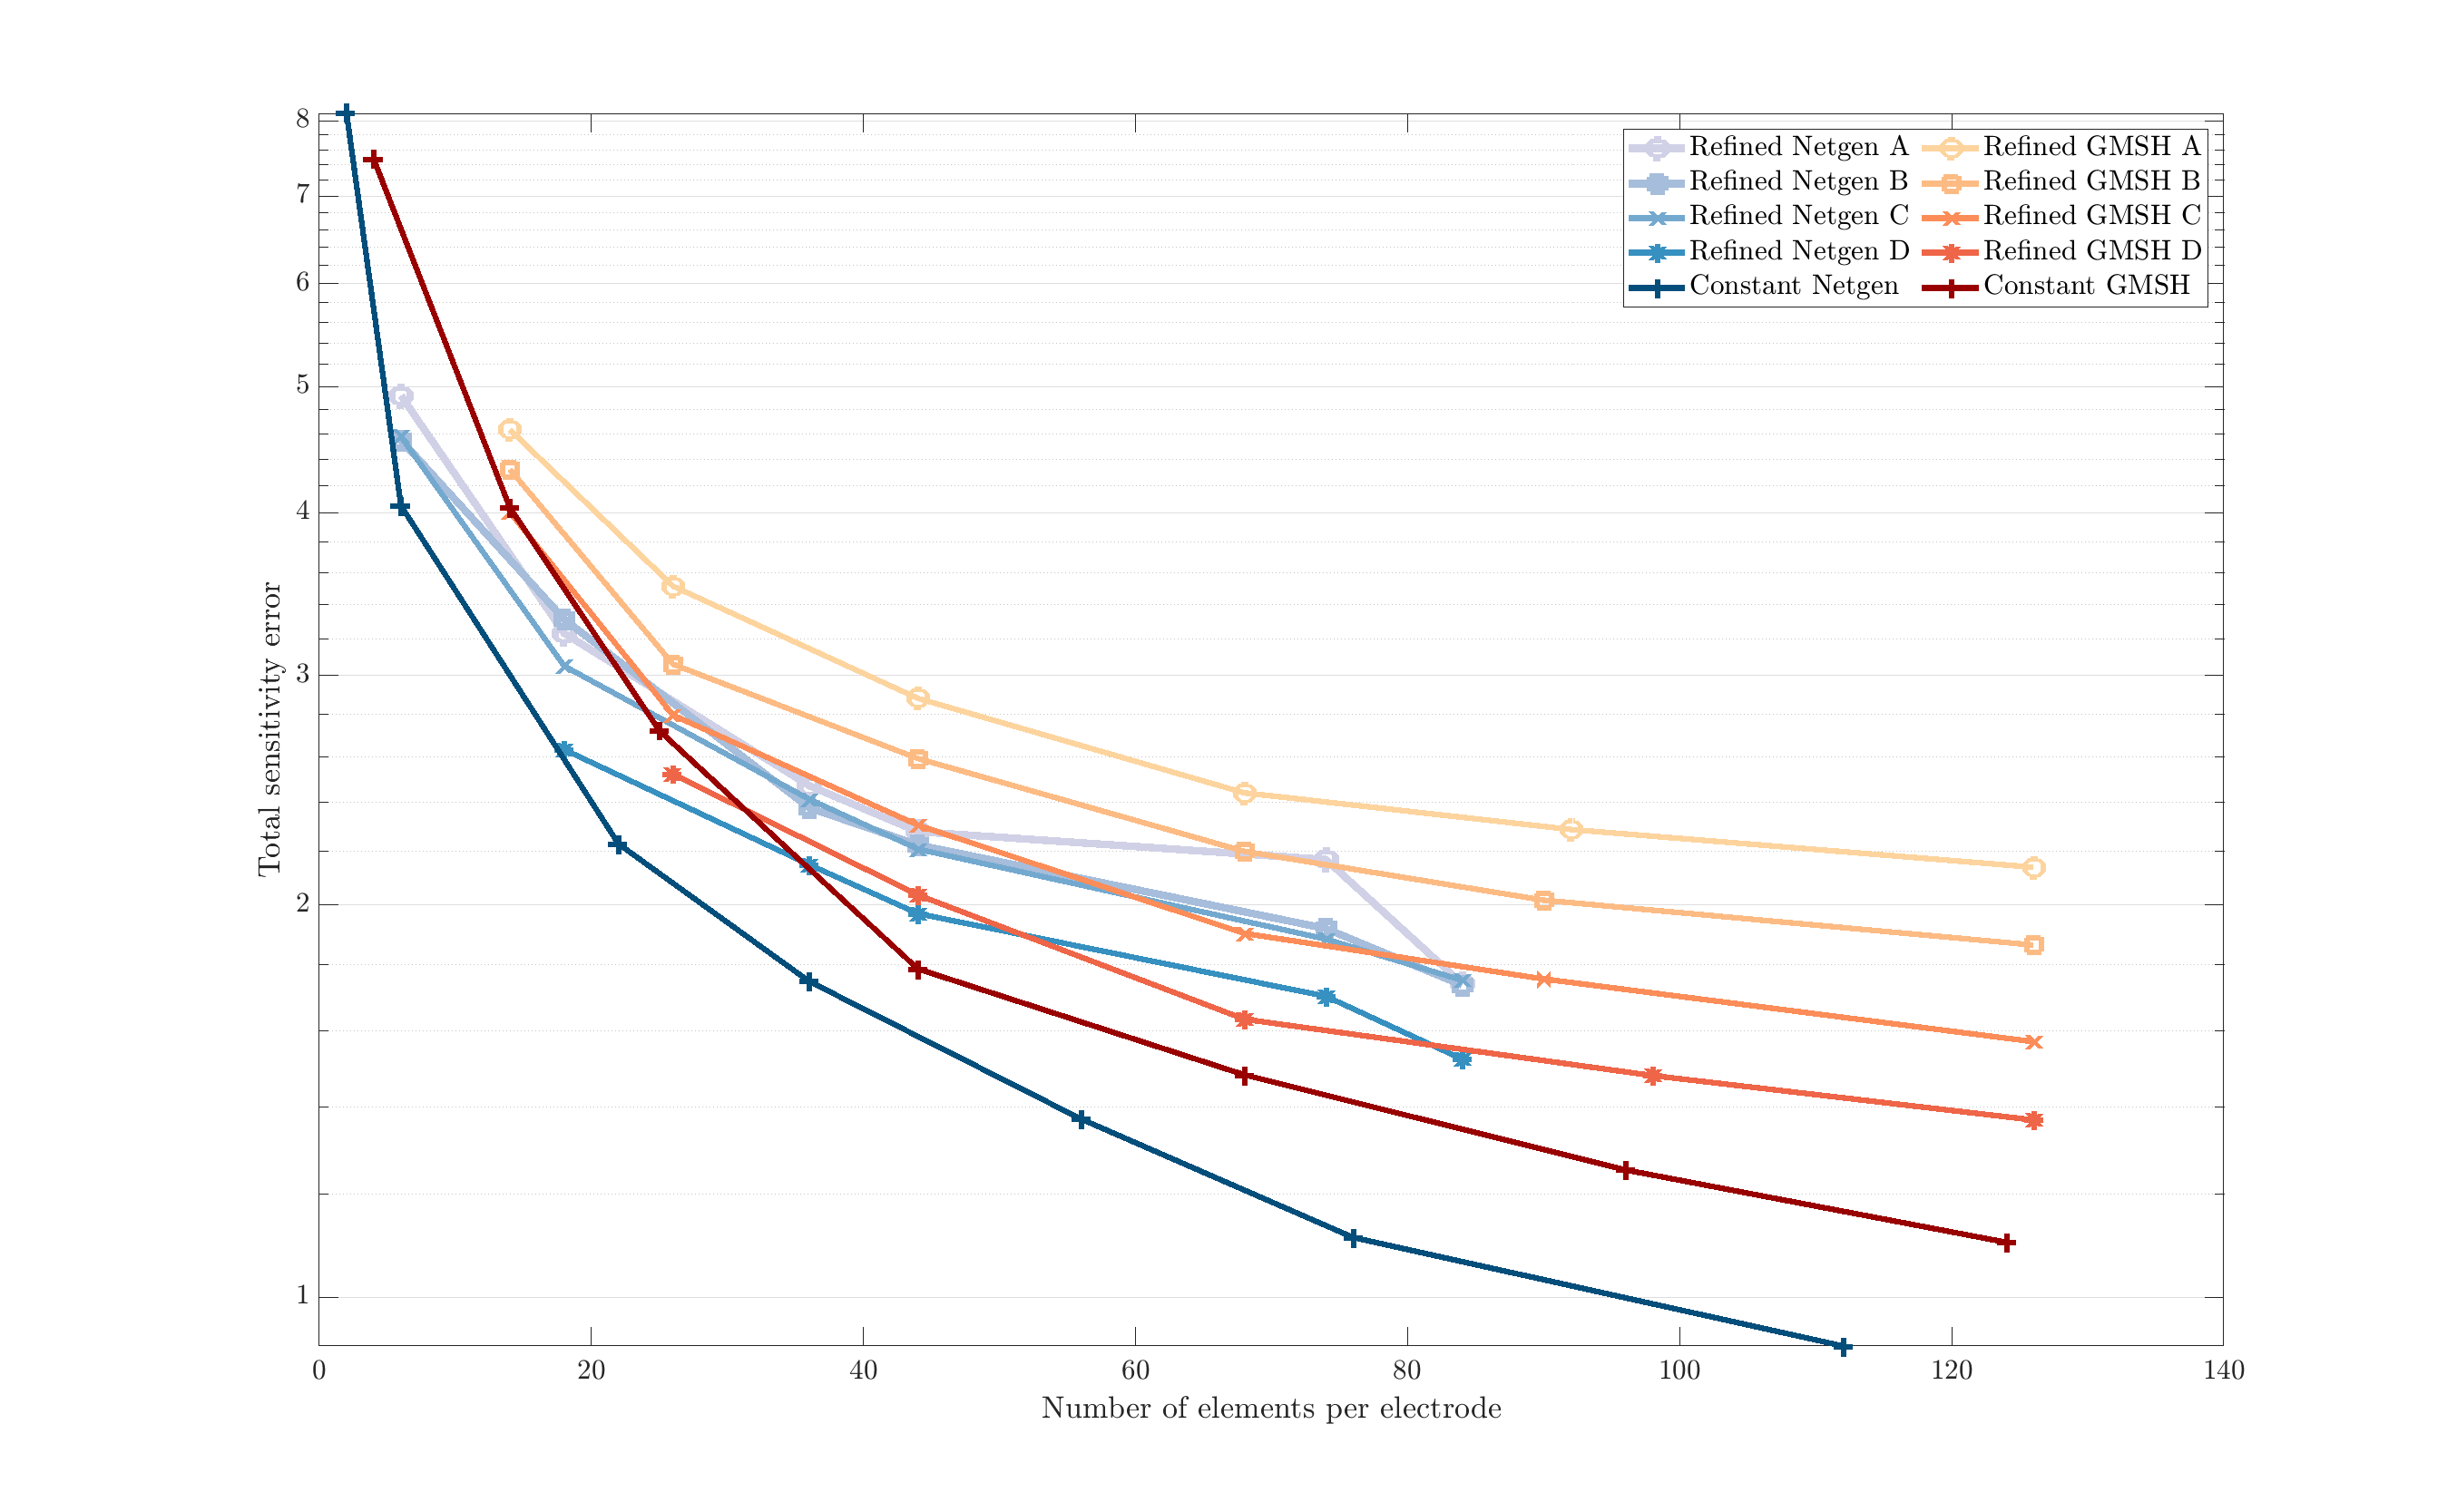
\includegraphics[width=\columnwidth]{chapter_3/imgs/sens_error_total.pdf}
  \caption[Mesh sensitivity error vs. elements per electrode]{\label{fig:results_sens_original} Sensitivity error of each mesh as a function 
  of the number of elements per electrode for both Netgen and Gmsh. The darkest lines indicate the
  constant mesh refinement, lighter lines indicate a larger maximum internal mesh size. The maximum
  internal mesh sizes are as follows: refinement A - 5 cm; refinement B - 4 cm; refinement C - 3 cm;
  refinement D - 2 cm.}
\end{figure}


Example sensitivity profiles for the M-series meshes are shown in \fref{fig:roiMethods}.
The resulting sensitivity profile near the electrodes more closely matched the reference case 
when refinement at the electrodes was higher. 

\begin{figure}
  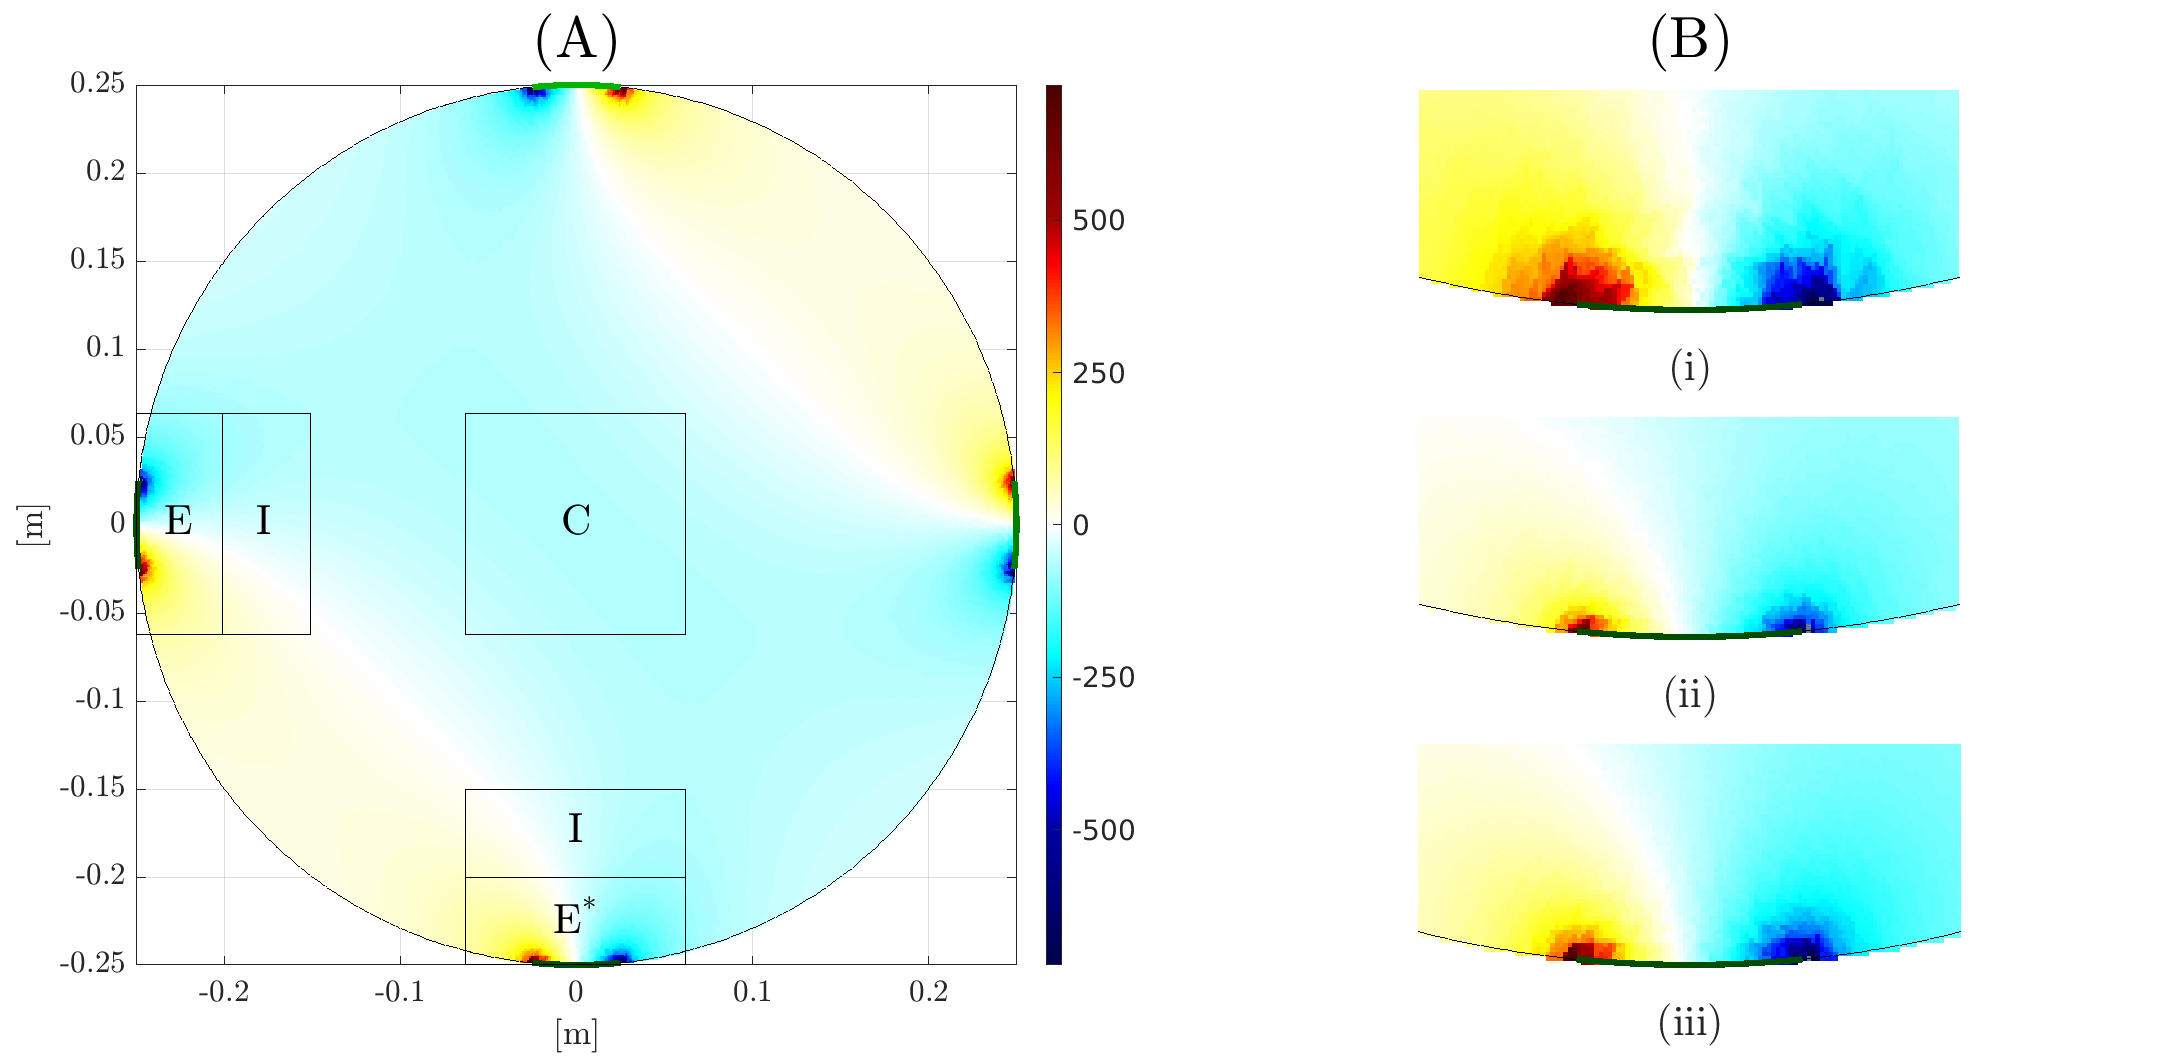
\includegraphics[width=\columnwidth]{chapter_3/imgs/roi_methods_figure.pdf}
  \caption[Sensitivity distribution and regions of interest]{\label{fig:roiMethods} (A) Sensitivity distribution for the reference mesh
  (C15) generated in Gmsh with regions of interest used to compare between models. 
  (B) 3 sensitivity distributions in region E\textsuperscript{*} next to the electrodes: (i) Constant mesh M1
  (ii) refined mesh M15 with a balance point of 82\% (iii) reference mesh from (A).
  }
\end{figure}

The total sensitivity error across all meshes is plotted vs. the balance point in
\fref{fig:balance_sens}. For meshes generated with Gmsh the minimum error was 
achieved when the node balance point was approximately 85\% of the model radius corresponding
to model M15-B, 
and for Netgen generated meshes the minimum sensitivity was achieved in model M13-A at a balance point
of approximately 70\%. Gmsh achieved a lower sensitivity error measured against
the respective reference mesh. For meshes using Netgen refinement, the balance point did not
increase evenly as the electrode density was increased and the internal density decreased. 
To maintain the same number of nodes within the model, Gmsh required a larger internal maxh
than Netgen. Gmsh generated meshes with more nodes for the same input
parameters, but  generally the resulting mesh sizes were closer to those specified. The
resulting mesh parameters for odd numbered meshes can be seen in \fref{tab:mesh-table}.
Across all meshes the measurement error when computing the voltage measurements was insignificant
at less than 0.2\%.

\begin{figure}
  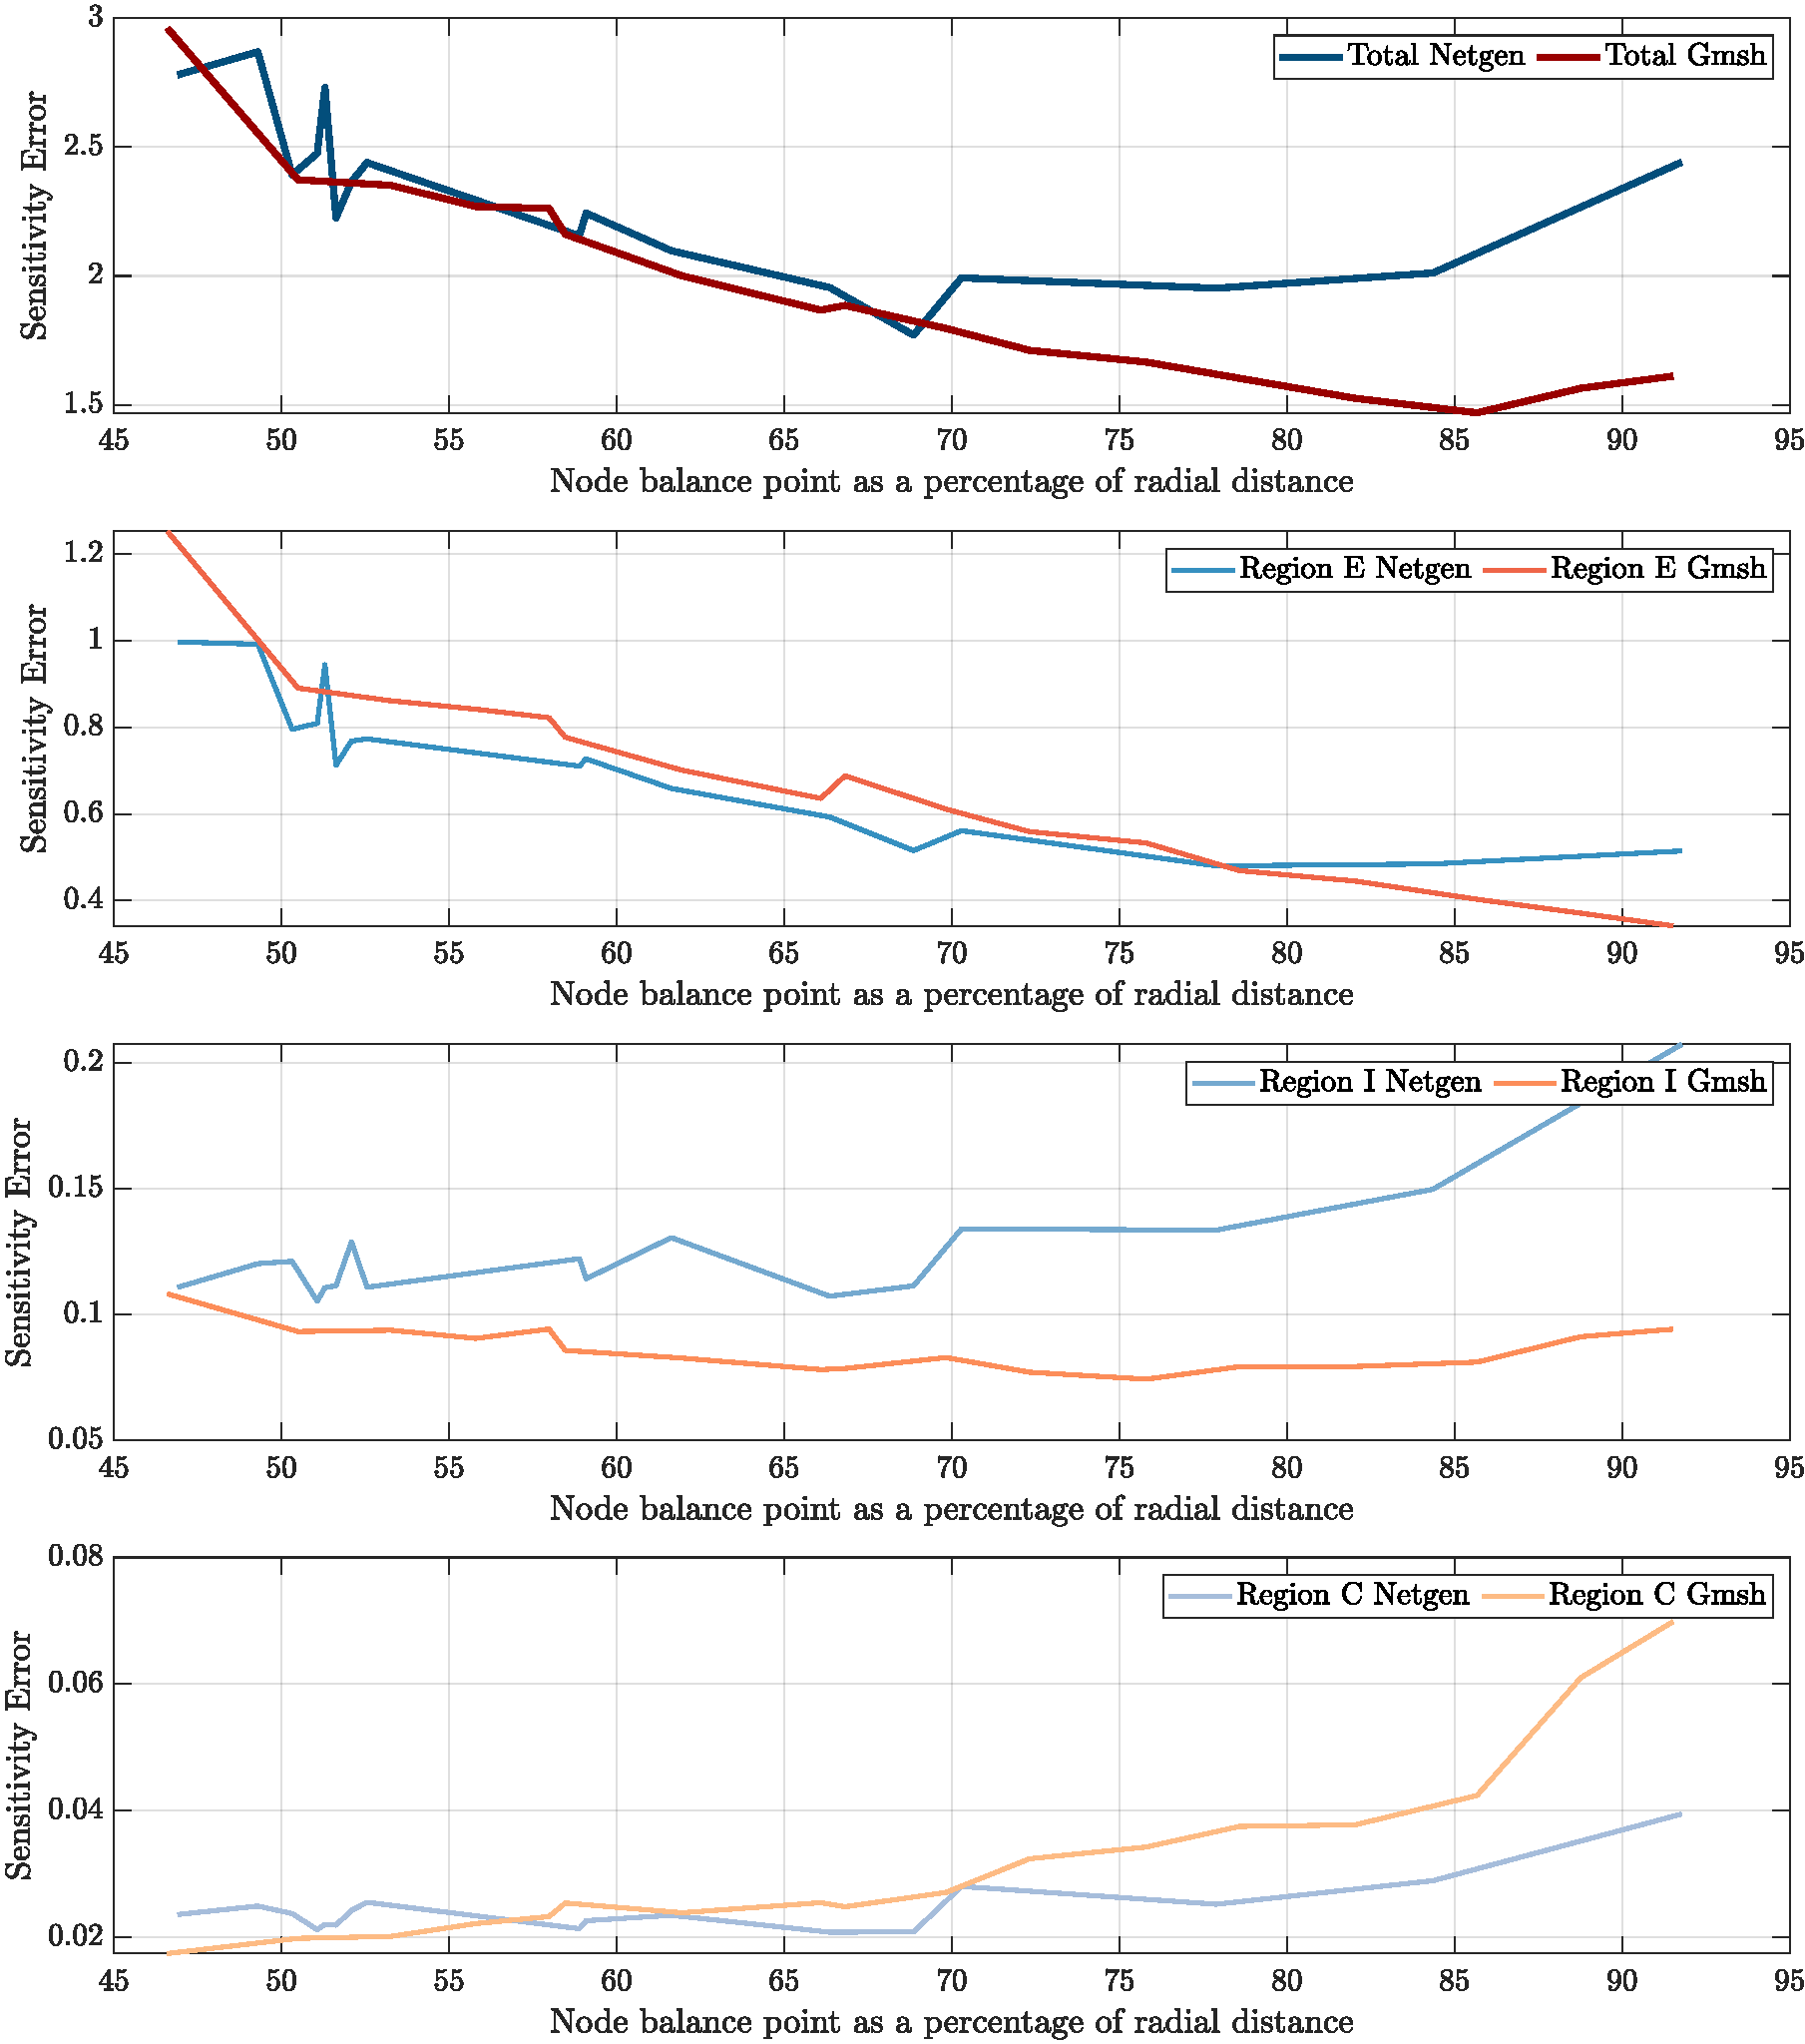
\includegraphics[width=\columnwidth]{chapter_3/imgs/m-mesh_sens_error_regions_split.pdf}
  \caption[Sensitivity error with shifting node balance]{\label{fig:balance_sens}
  Resulting sensitivity error for Netgen (blue) and Gmsh (red) as the balance of the nodes
  was shifted towards the electrodes. From top to bottom: total sensitivity error, the sum of 
  sensitivity error in region E, the sum of sensitivity error in region I and the sum of
  sensitivity error in region C. The regions are described in \fref{fig:roiMethods}.}
\end{figure}

  
%  Results show that for both Netgen and Gmsh there is a significant decrease in measurement error 
%  as the number of elements throughout the model is increased. This is shown in Fig.~\ref{fig:results_meas} 
%  where the measurement error on refined meshes decreases as the models are generated with a higher 
%  density of elements. 
%  
%  For both Netgen and Gmsh when using mesh refinement techniques there was no change in the measurement error when compared to 
%  the coarsest models. % THIS DOES NOT MATCH EARLIER RESULTS WHAT IS GOING ON NOW?!?!
%  
%  When comparing mech quality based on the average minimum angle in the tetrahedra, Netgen was shown to have a higher 
%  quality mesh for constant models, but when using refinement Gmsh meshes had a better overall minimum angle score. 
%  These results are presented in Fig.~\ref{fig:results_qual} 
  
\section{Discussion}

We consider several questions on the requirement of FEM refinement in the neighbourhood of
electrodes and the available tools for mesh refinement in EIT. 
1) Given a ``FEM element budget'', what should
balance of nodes be between the centre of the model and the electrodes?
2) How do different freely available meshing tools that are
commonly used with EIT compare when used to refine 3D meshes?

While refining meshes surrounding the electrodes  is agreed to be useful,
there is a lack of systematic analysis of
the required refinement level, and controlling such
refinement is difficult. Automatic mesh refinement is an area of active work and there are
a number of commercial and free products available. We compare two programs 
used widely in EIT.
Our results show that Netgen and Gmsh control mesh refinement differently 
and the same input parameters result in meshes with different numbers of nodes. 
\fref{fig:electrode_mesh_size}, depicts the difference in
mesh dissipation rates between Netgen and Gmsh. The mesh size in Gmsh increased
gradually from the surface of the electrode  towards the centre of the model,
where the mesh size in Netgen increased much more quickly from the edges of the
electrode. While we attempted to control the dissipation rate in 
Netgen by manipulating the mesh density in the centre of the model, we were unable 
to achieve a smooth transition between the electrode and internal regions of the mesh. 

To analyze the benefit of electrode refinement and the difference between 
Netgen and Gmsh refinement techniques we consider
a sequence of refined meshes compared to a ``gold standard'', uniformly fine
FEM solution. The models were refined either globally or in the electrode
neighbourhood, and the error in the sensitivity matrix $\bf J$ %voltage measurement,  and mesh quality %current distribution and sensitivity
was compared. \fref{fig:results_sens_original} displays the difference 
in sensitivity between constant meshes and meshes with refinement at the electrodes. 
The sensitivity error was lower in Netgen across all constant refinement meshes, in
part because there were more total nodes than Gmsh meshes with the same number
of nodes on the electrode. Refinement around the electrode decreased the total 
sensitivity error, but still had larger error than meshes with constant refinement 
due to the smaller number of nodes in the model. 

Using the balance point analysis, we were able to determine the optimal distribution
of nodes to minimize sensitivity in both Gmsh and Netgen. The minimum total sensitivity 
from \fref{fig:balance_sens} was approximately 70\% for Netgen. This was mainly 
due to the rapid dissipation of node density away from the electrodes. Increasing 
the refinement near the electrode reduced
error in region E, but in region I there were insufficient
nodes to reduce the sensitivity error. As the balance of refinement approached
90\% the error in region E also started to increase as the node density did not remain
fine throughout the entire region. This effect can also be seen in \fref{fig:electrode_mesh_size}.
In Gmsh the optimal balance for refinement was at approximately 85\%
of the radial distance. Since mesh density was set to reduce evenly 
between the electrode surface and the centre of the model, there 
was a higher density of nodes that was maintained in regions E and I as the 
electrode refinement increased. The error in the centre of the model 
was higher in Gmsh meshes, but since this is where the sensitivity is 
lowest the total sensitivity error was much lower. 

The ability to selectively control the mesh refinement in regions in Gmsh also allows 
users to generate complex meshes and control mesh density surrounding internal structures 
and electrodes an example mesh is shown in \fref{fig:adv_mesh} where a model was
created of
a probe entering a bone from the surrounding tissue. 
These additions fill an important need in EIT to allow for more accurate models 
of regions surrounding internal structures and electrodes, and 

\begin{figure}
  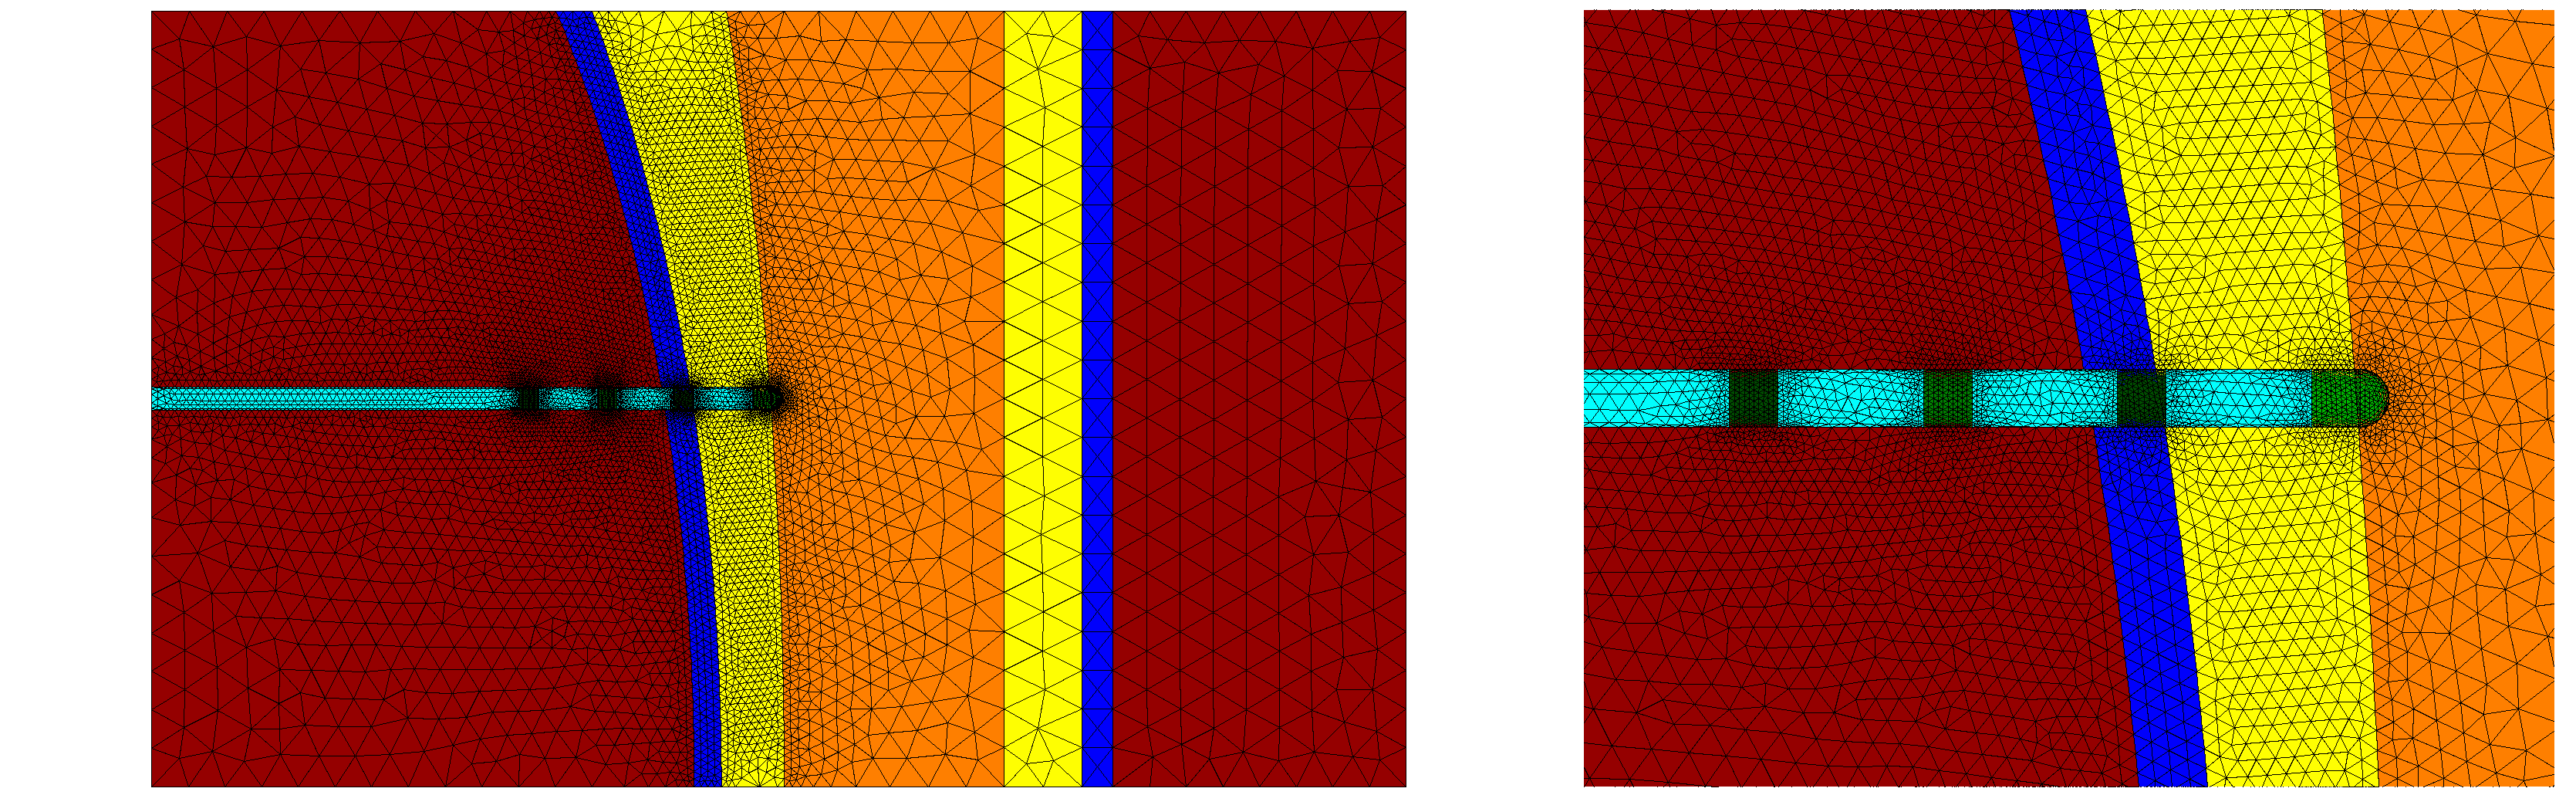
\includegraphics[width=\columnwidth]{chapter_3/imgs/advanced_mesh_combined.pdf}
    \caption[Advanced mesh example of an internal probe]{\label{fig:adv_mesh} Example FEMs of a probe entering a bone from the surrounding 
    tissue. Refinement is specified around the electrodes and tissue interfaces near the probe.}
\end{figure}

Despite the increased ability to control refinement, the results still show that there are
discrepancies between the specified parameters and the resulting meshes. The data in 
\fref{tab:mesh-table} show that the maximum element lengths specified for each mesh 
were different from the actual maximum edge lengths. As the node density was increased
near the electrodes, in Netgen the balance point did not always shift towards the electrode
as the maximum node density was not always higher despite specifying a smaller mesh size.
In Gmsh the mesh density was closer to the specified values, typically resulting in more
nodes in the refined meshes. 

Across both analyses errors away from the refined areas may be higher,
but the ability to refine meshes selectively near regions where high sensitivity 
is required may allow for reduced measurement error while still allowing for quicker 
meshing times.
As more electrodes are added and the model complexity is increased, we expect that 
refinement around the electrodes will continue to reduce total sensitivity error. However 
the node balance analysis will not be possible for irregularly shaped models.
The node balance analysis provides a straightforward method to determine the 
ideal placement of a given number of nodes to reduce model errors.

% Based on these results, we produced an additional model combining the electrode
% refinement of R8 and the maximum element size of C5 (18947 nodes and 98595
% elements). Its sensitivity
% error near the electrode was better than C2, while deeper in the medium it was
% on par with C5.  It produced measurement error of only 0.11~mV.


\section{Conclusion}

In summary, as expected, refinement of  meshes near electrodes 
does improve model accuracy in terms of sensitivity.
We recommend that, for each EIT imaging case, required model accuracy be
determined from an analysis of the system, 
and to minimize the sensitivity error in the forward solution 
the balance of the nodes should be approximately 
85\% towards the radius of the
model when the dissipation of mesh refinement is constant. 
\chapter{Custom Meshes from CT Images}

\section{EIT for ARDS Patients}

\section{A Segment Editor Program}

\subsection{Automatic segmentation of the thorax}
\begin{algorithm}[H]
	\SetAlgoLined
	\KwIn{image}
	\KwOut{external boundary}
		weiner filter\;
		Set the lung intensity to 0\;
		erode image using disk size 20\;
		reconstruct on image from line 4\;
		dilate with disk of size 20\;
		reconstruct on image from line 6\;
		binarize, thresh = 0.5\;
		fill holes\;
		close - disk of size 2\;
		open using disk size 5\;
		external boundary = largest object\;
	\caption{Segment the external body boundary.}
\end{algorithm}

\subsection{Manual Segmentation Correction}

\subsection{Mesh Generation}
\subsubsection{Extruded Geomerty}
\subsubsection{3D Lung Regions}


\section{Evaluation on ARDS Patients}

\subsection{Methods}
\subsection{Results}
Data from 4 ARDS patients with CT
and EIT were used to develop a segmentation 
and correction tool to identify 
the lungs and boundary of the body.  
Segmentation was done using the 4th intercostal space, 
with 10 adjacent CT 
slices to form an enclosed chest cavity. 
The lungs
and exterior boundary were identified by increasing the contrast
and identifying an appropriate threshold.
Each segmentation was downsampled to
20 points that could be edited by the user in Matlab. The 
mesh was generated using 
\verb!ng_mk_extruded_model!~\cite{Grychtol2012} in EIDORS 
3.10~\cite{Adler2019}. Images were reconstructed 
using GREIT~\cite{Adler2009}. 
The GI index was calculated using the method
presented by Zhao et al.~\cite{Zhao2009} using the lung regions from the 
forward model. A ventilated lung estimate was made using the
segmentation as $\frac{A_{\text{ventilated lung}}}{A_{\text{total lung}}}$.
%by dividing the area of healthy lung by 
%the total lung area
%from the automatic segmentation.

\begin{figure}
\centering
% Use the following line with your images (pdf preferred)
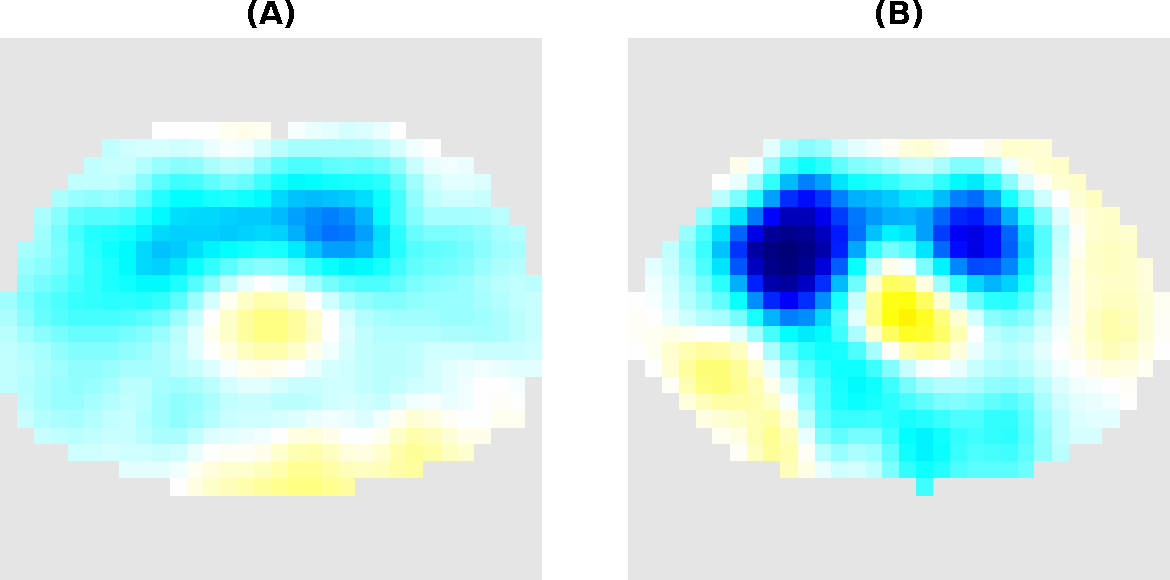
\includegraphics[width=\textwidth]{chapter_4/imgs/basic_vs_advanced_3_cropped.pdf}
\caption{\label{fig:ct_mesh_breath}%
Single breath using: A) generic model B) custom model
}
\end{figure}

Results in fig.~\fref{fig:breath} show a reconstructed image 
with more separable lungs in the enhanced model, and a mean GI index for each breath in the 
1 minute 
recording that follows 
trend of the ventilated lung percentage in table~\ref{tbl:twocol}.

\begin{table}
  \centering
  \caption{\label{tbl:twocol} %
  Ventilated lung estimate vs. GI index scores.}
  \begin{tabular}{|p{1.2cm}|p{1.5cm}|p{1.8cm}|p{1.7cm}|}
    \hline
  Subject & Ventilated lung (\%) &
  GI (basic model) & GI (custom model) \\ \hline
  1 & 99.9 & 0.353\pm0.004& 0.690\pm0.005 \\ 
  2 & 85.5 & 0.640\pm0.022& 0.771\pm0.020  \\
  3 & 79.6 & 0.695\pm0.007& 0.857\pm0.009  \\
  4 & 27.0 & 0.614\pm0.011& 1.81\pm0.053 \\\hline
  \end{tabular}
  \vspace{-1em} 
\end{table}


\begin{figure}
\centering
% Use the following line with your images (pdf preferred)
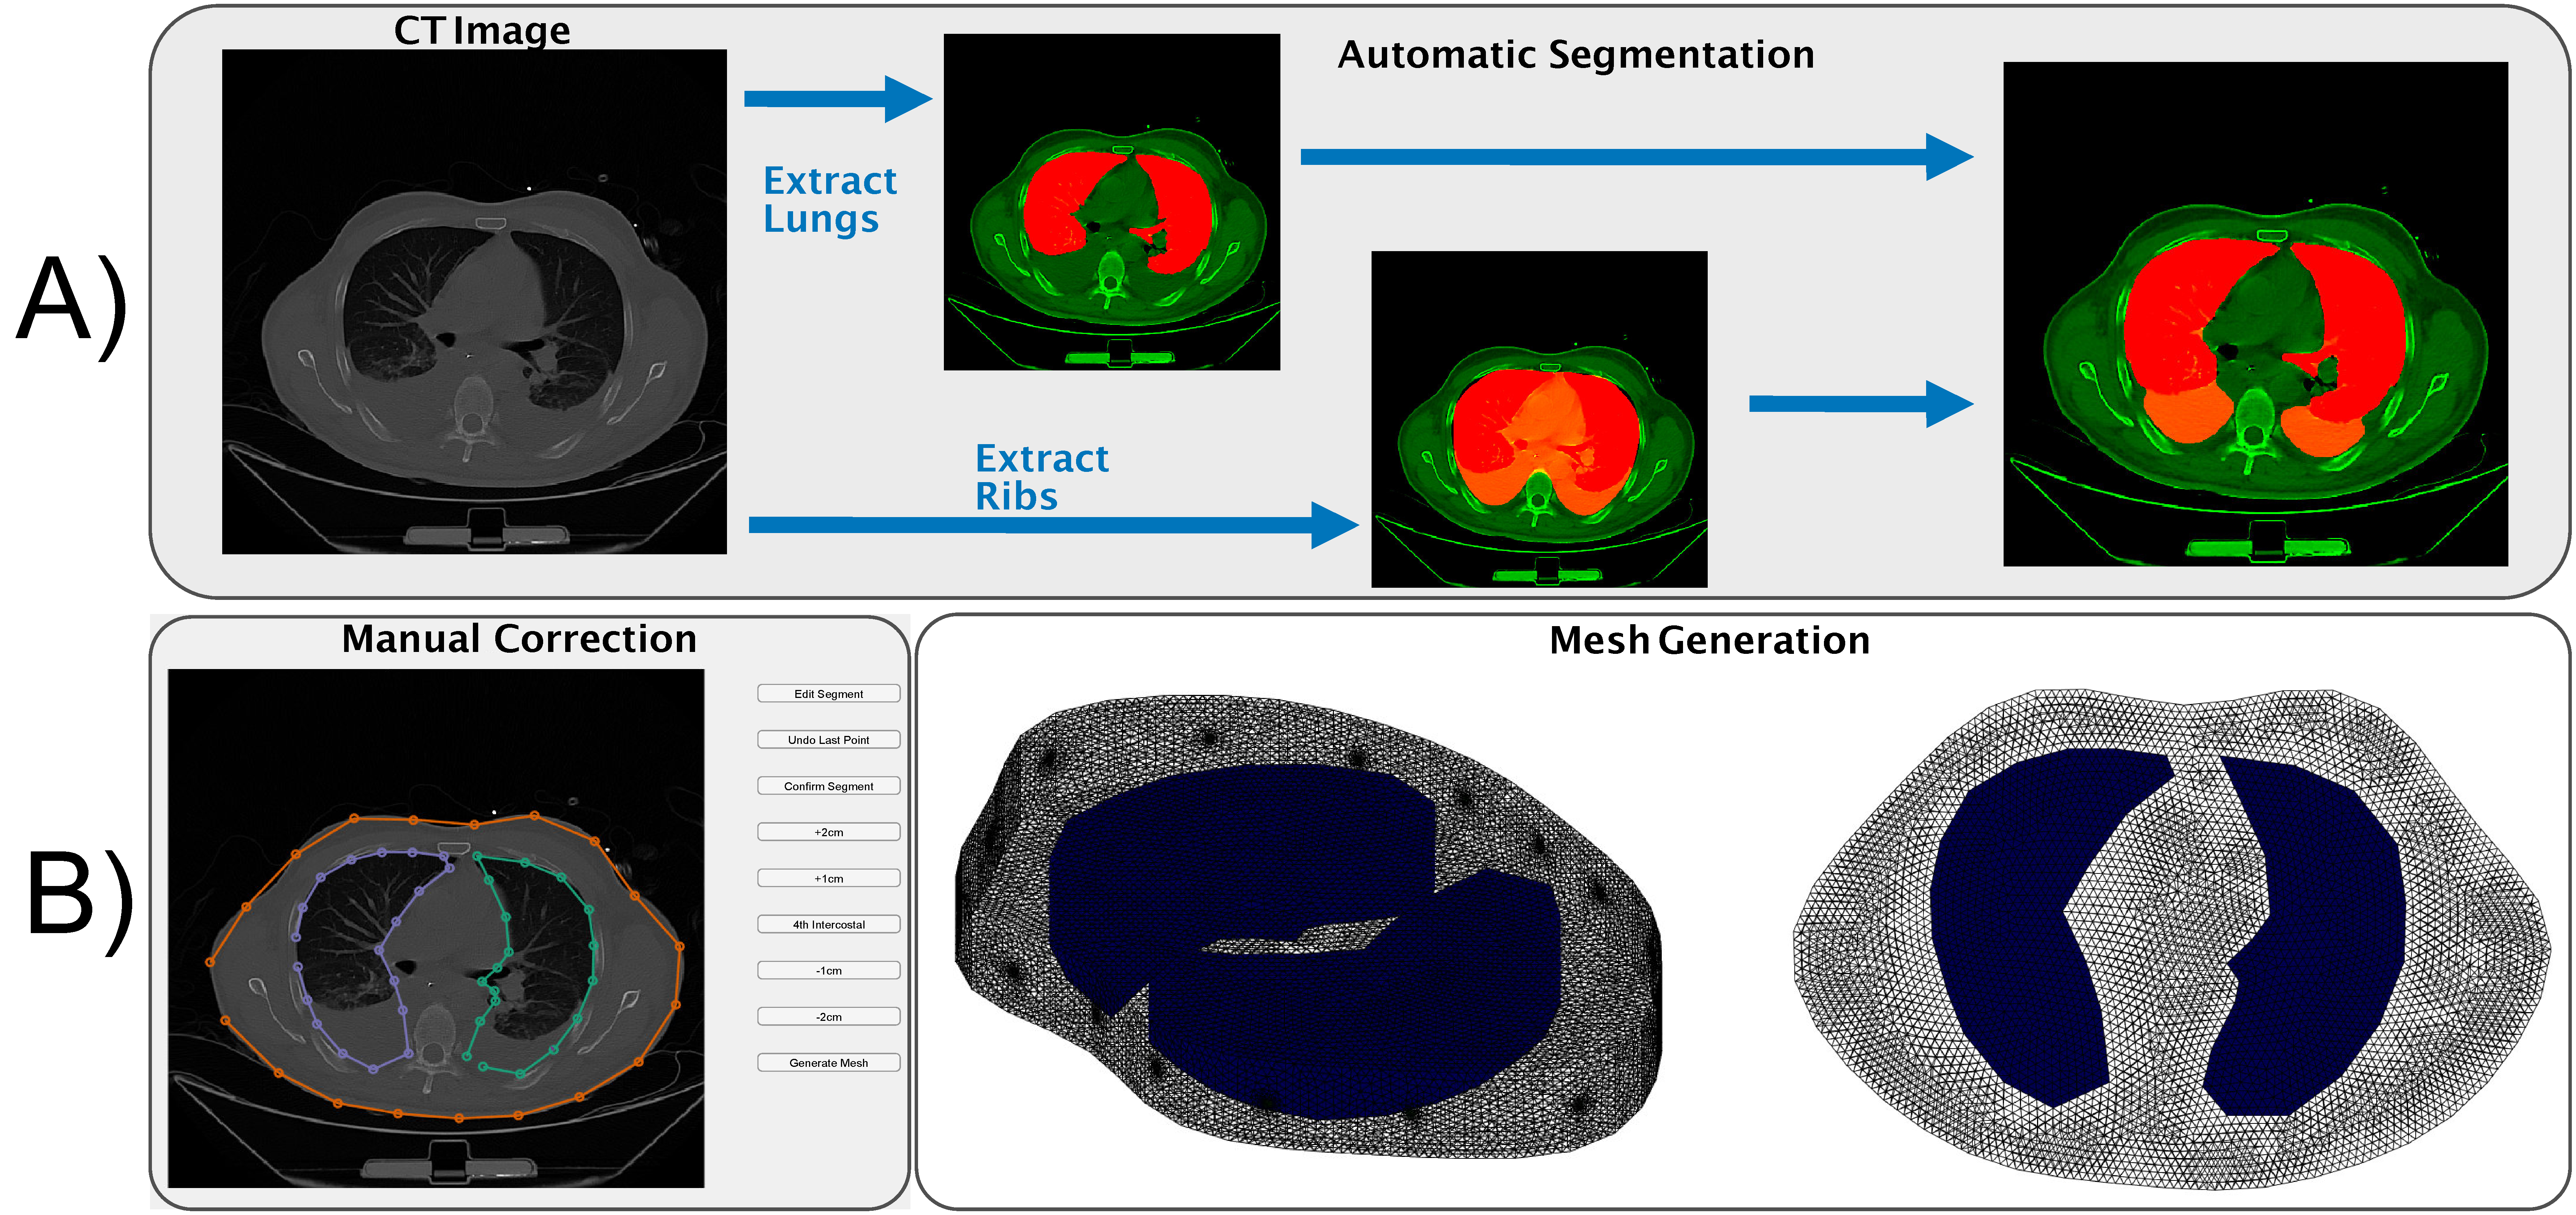
\includegraphics[width=\textwidth]{chapter_4/imgs/methods_figure.pdf}
\caption{\label{fig:segment_overview}%
An overview of the segmentation and editing process showing: 
A) A sample raw CT which was thresholded, scaled and adjusted over several 
adjacent slices to identify
the lung regions and an enclosed rib area, and the resulting lung estimate; and
B) A screen  capture of the manual mesh correction process and 2 views of the generated
mesh.
}
\end{figure}
\chapter{Internal Electrodes}
%\subsection{The effects and uses of internal electrodes on 3D EIT image reconstructions}

\section{Motivation}
One of the shortcomings of EIT is low sensitivity away from the electrodes. 
For continuous monitoring of cardiac-related events an EIT protocol with an improved sensitivity 
near the heart and innermost regions of the lings may improve results and imaging accuracy.

EIT has low sensitivity away from the electrodes which are typically placed on the body surface. 
This chapter will investigate the use and application of internal electrodes and quantify the improvement 
in sensitivity and image reconstruction accuracy in simulation.

\section{Summary}
This chapter provides proof of principle of internal electrode configurations to 
improve EIT sensitivity and reconstruction accuracy.
The goal of this chapter is to determine the viability of internal electrode use through a series of simulations and phantom measurements then validate
the imaging ability using one or two animals. 

We expect to show that using internal electrodes increases the sensitivity of the measurements to internal impedance changes 
and enables a higher resolution of image reconstructions in these central regions of the thorax. 

\section{Simulations}
To analyze the sensitivity changes due to different electrode 
configurations finite element models (FEMs) of a cylindrical tank were 
created with each of the tested electrode configurations. Figure~\ref{fig:tank_FEM} shows the four 
different configurations that were tested: a 2D 
electrode ring of 32 electrodes; a 3D configuration of 2 layers of 16 
electrodes (3D(a)); a second 3D configuration of 2 layers of 15 electrodes 
plus 2 central internal electrodes inline with the electrode planes (3D(b)); and a final 3D configuration of 
2 layers of 14 electrodes with 4 central internal electrodes evenly spaced between the electrode planes (3D(c)).

\begin{figure}
\centering
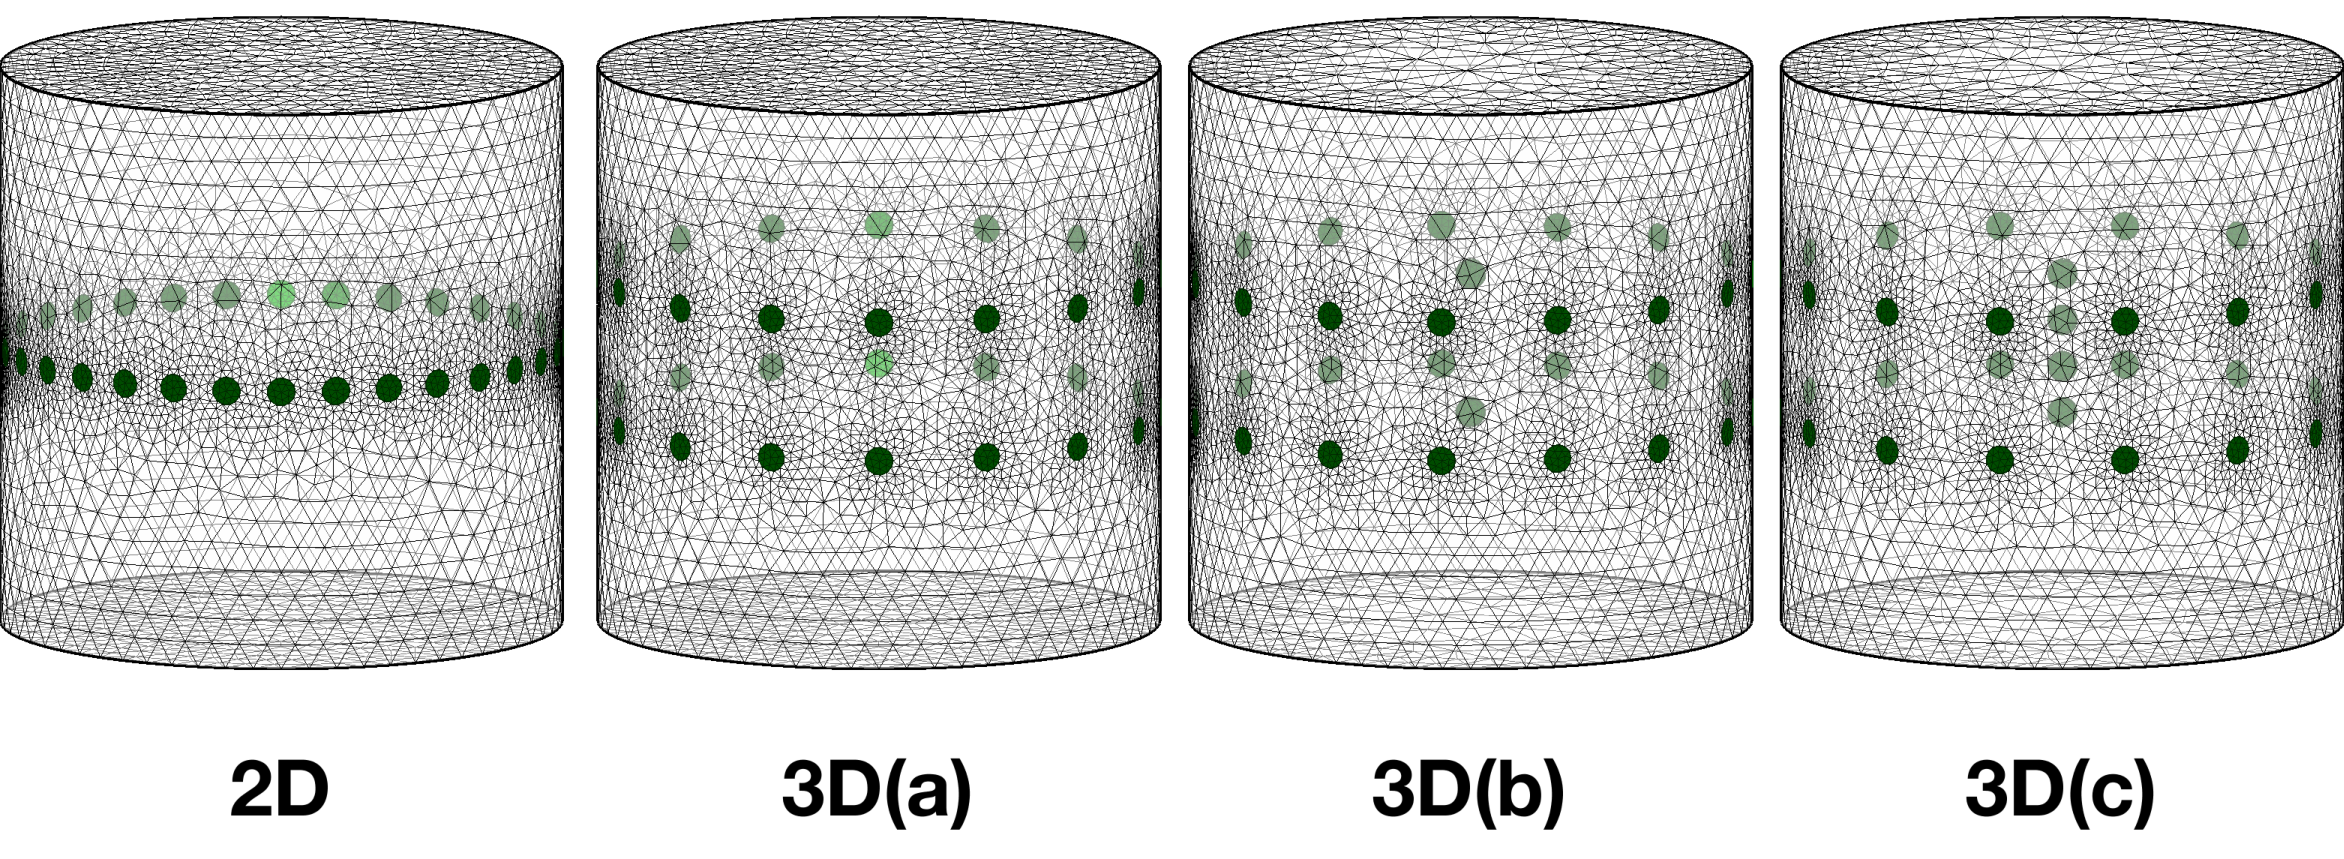
\includegraphics[width=\textwidth]{chapter_5/imgs/FEM_Comparison.pdf}
\caption[Internal electrode configurations]{4 configurations of electrodes were tested: 2D) a single ring of 32 electrodes; 
	3D(a) 2 rows of 16 external electrodes; 3D(b) 2 rows of 15 external electrodes with 2 internal electrodes; and 3D(c) 2 rows 
of 14 external electrodes and 4 internal electrodes.}
\label{fig:tank_FEM}
\end{figure}

The tank in the simulations has a height of 2 m, radius of 1 m, and the electrode radius
is 0.05 m for both the round external electrodes and the spherical internal electrodes.
In the 3D configurations the plane separation is 0.5 m and in all configurations the radial
spacing between electrodes is equal.
The background conductivity of the tank was 1 S/m and the conductivity of the target was
10 S/m.

When reconstructing images a conductive target was added to the tank
centred at a height of 1 m at the midpoint of the tank radius. The target
object radius is 0.4 m.

The reconstructions of the conductive object with and without additive noise are shown in Figure~\ref{fig:reconstruction_comparison}.
To generate EIT images from voltage measurements, the 3D GREIT
reconstruction algorithm
was used~\parencite{Adler2009}. A spherical
conductive target with a radius of 20\% of the tank radius
was placed midway between the centre and boundary
of the tank, in a region with typically low sensitivity.
The inverse problem hyperparameter
was selected so that in all instances the amount of measurement
noise that propagated from the measurements into the final images
was equal.

Preliminary reconstructions on simulated data show that internal electrodes are able to reconstruct a conductive object closer to its true 
size based on visual inspection, but more simulations are required to quantify the improvements. These preliminary reconstructions are shown in
Figure~\ref{fig:reconstruction_comparison}. The top row shows reconstructions with no additive noise, and the second row shows reconstructions on measurements with 5dB of 
additive noise.

\begin{figure}
\centering
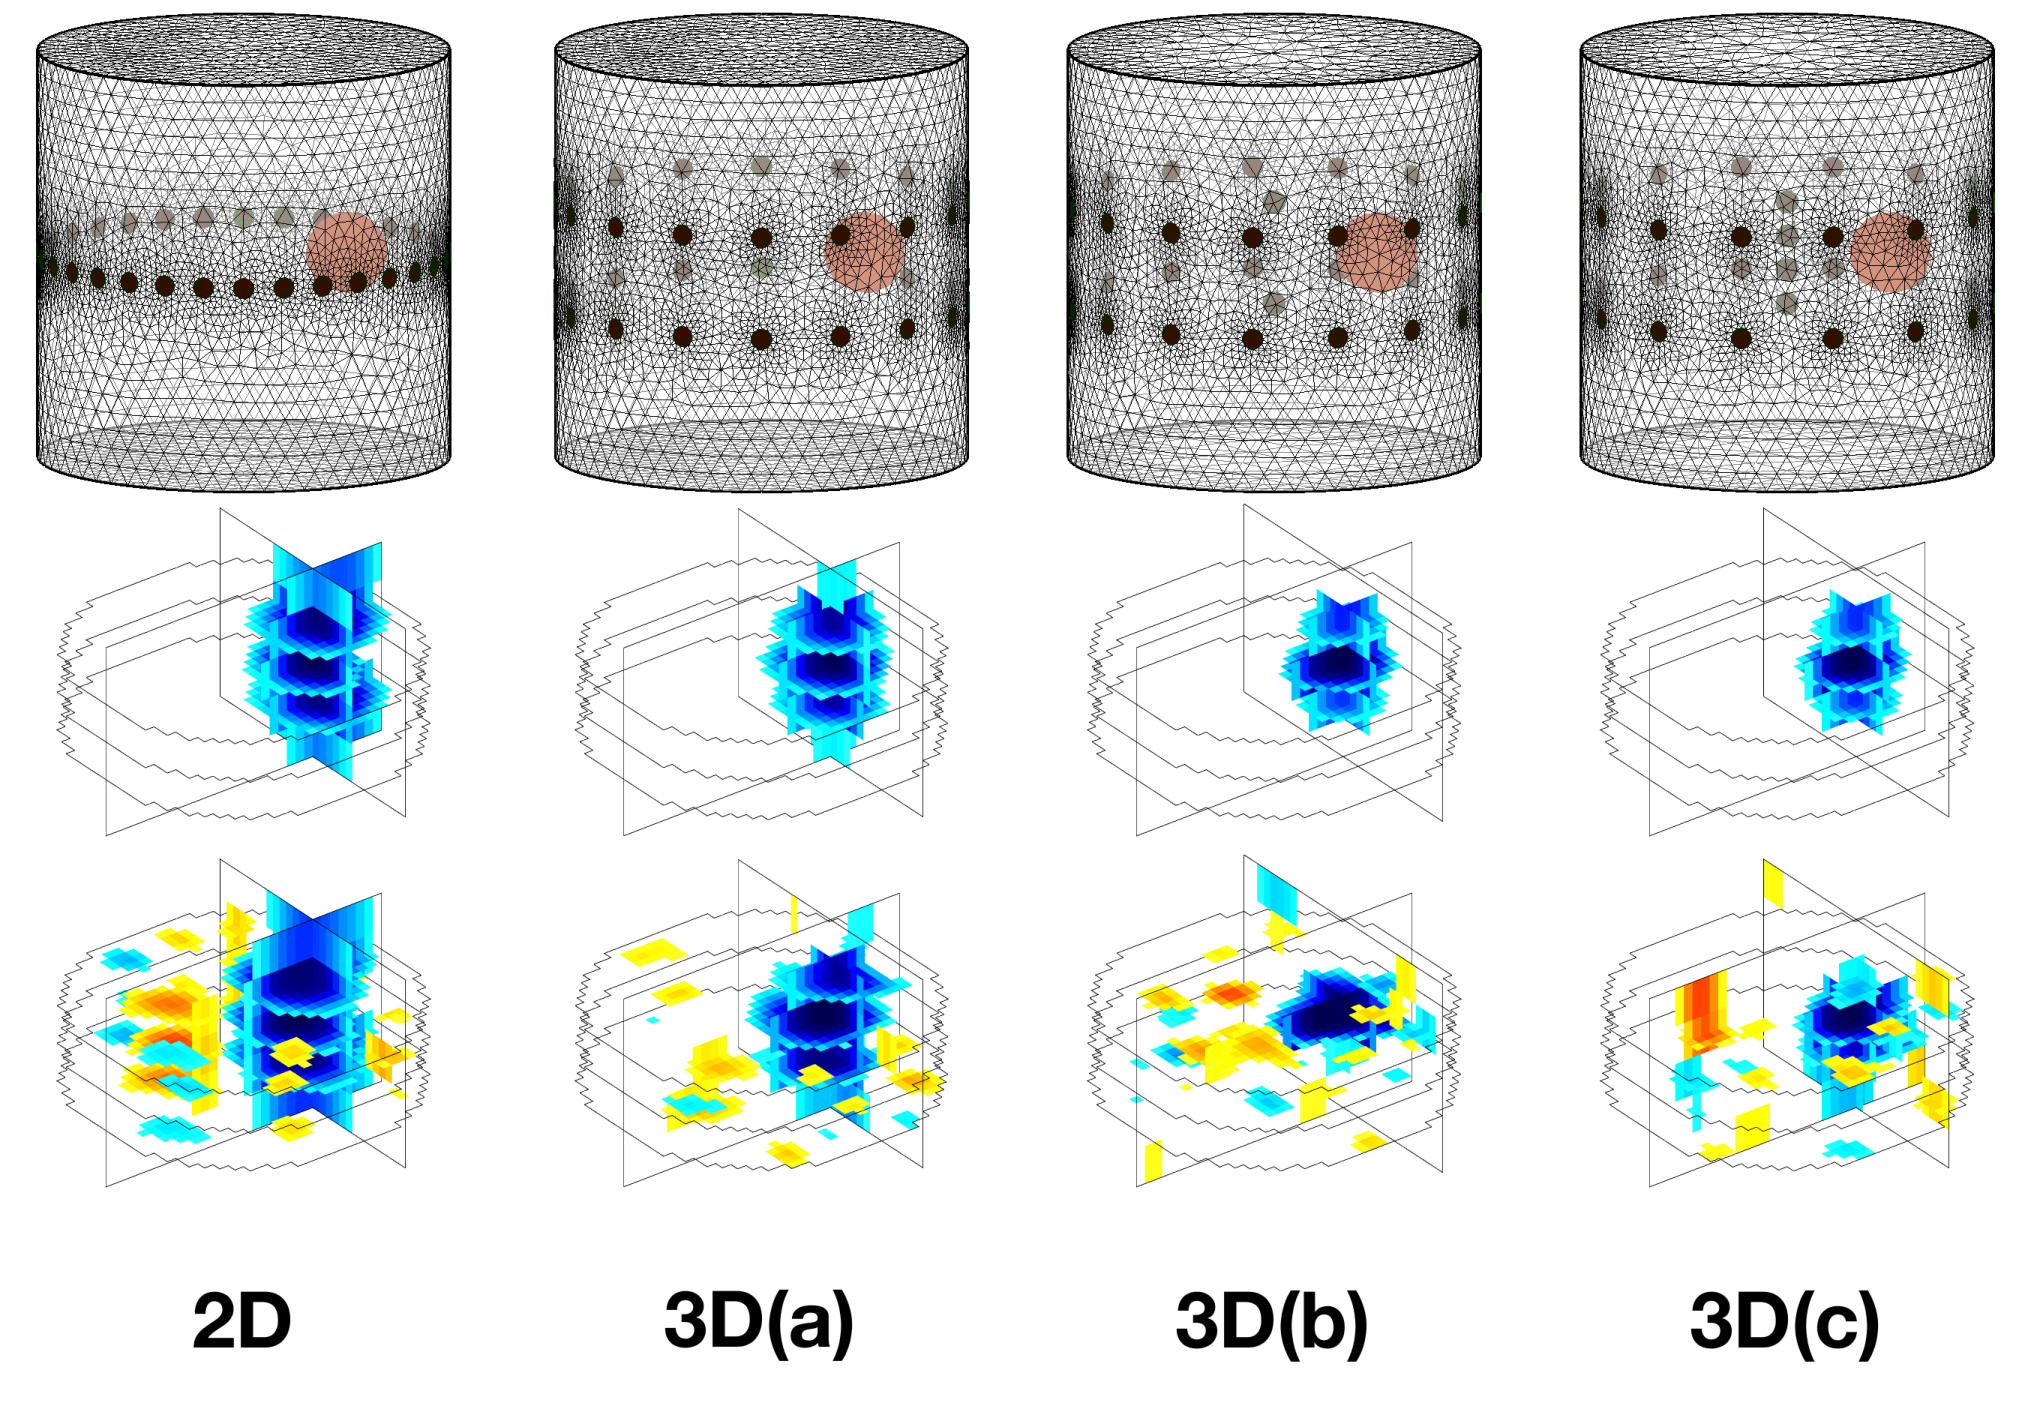
\includegraphics[width=\textwidth]{chapter_5/imgs/Image_Comparison.pdf}
\caption[Internal electrode simulation reconstructions]{The top row shows reconstructions with no additive noise, and the second row shows reconstructions on measurements with 5dB of
additive noise.}
\label{fig:reconstruction_comparison}
\end{figure}

Preliminary results shown in Figure~\ref{fig:internal_sensitivity} show internal sensitivity distribution changes when using 2 and 4 internal electrodes compared to the
typical 2D and 3D configurations with only external electrodes. 


\begin{figure}
\centering
%\includegraphics[trim=0 65 0 400,clip,width=\textwidth]{chapter2/imgs/Sensitivity_Comparison_new.pdf}
\includegraphics[width=\textwidth]{chapter_5/imgs/Sensitivity_Comparison_new.pdf}
\caption[Sensitivity with different internal electrode configurations]{Sensitivity distributions for electrode patterns from left to right: A single 2D electrode plane; 2 electrode planes of 16 electrodes 
each; 2 internal electrodes and 2 external electrode rings of 15 electrodes; 4 internal electrodes arranged between 2 planes of 14 external
electrodes}
\label{fig:internal_sensitivity}
\end{figure}

The sensitivity is then calculated from the jacobian ($J$)of  the reconstruction matrix as:
% Sens = log(sqrt(sum(J.^2))'./get_elem_volume(fmdl_3dc));
$$ S = \frac{\sqrt{\sum_{i}\vec{J}_{ij}^2}}{V_i}  $$
where $V_i$ is the volume of each respective voxel. 

These results show the expected increased sensitivity in the central regions of the model. To further improve internal sensitivity a new
measurement pattern is proposed that uses more measurements between the internal probe and peripheral electrodes. The proposed injection and measurement
pattern is shown in Figure~\ref{fig:modified_measurement}.
The sensitivity of the proposed pattern was compared to the sensitivity profile of the same configuration using 
the basic ``skip 4'' injection and measurement pattern which has been found to 
give good sensitivity in 2D and 3D external electrode configurations~\cite{Grychtol2016}.

\begin{figure}
\centering
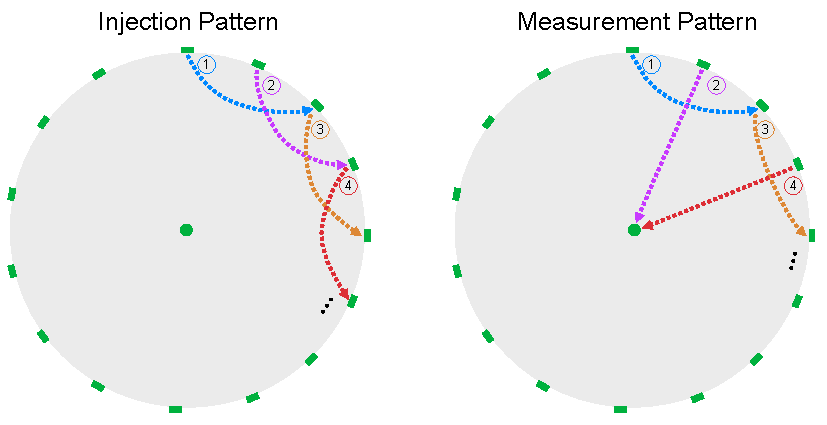
\includegraphics[width=\textwidth]{chapter_5/imgs/current_injection.pdf}
\caption[Current injection patterns with internal electrodes]{A proposed current injection and measurement pattern for \acrshort{eit} imaging with 2 internal electrodes.
The injection pattern is a typical ``skip 4 '' pattern injecting between every 5\textsuperscript{th} electrode in a square electrode layout and the
measurement pattern replaces every 2\textsuperscript{nd} measurement in the typical method with a measurement between the internal probe and
external rings. Note: this figure does not differentiate between upper and lower electrode planes, but all injections and measurements are done between 
the 2 planes.}
\label{fig:modified_measurement}
\end{figure}

Using this injection pattern preliminary results show a further increase in sensitivity in the internal regions without increasing the measurement
acquisition time. The sensitivity distribution for the new injection pattern is pictured in Figure~\ref{fig:modified_measurement_sens}.

\begin{figure}
\centering
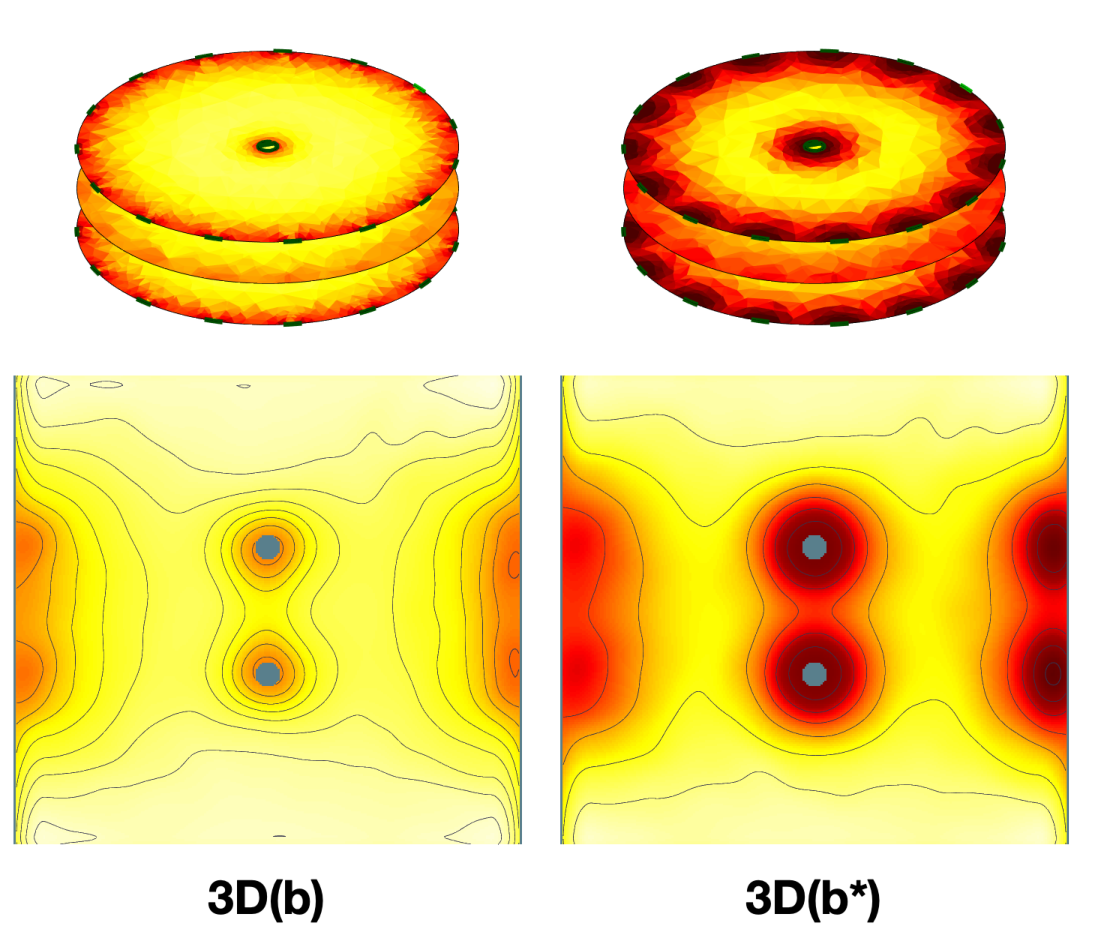
\includegraphics[width=\textwidth]{chapter_5/imgs/Injection_Comparison.pdf}
\caption[Sensitivity using internal electrodes with modified injection patterns]{A comparison between the sensitivity distributions for a typical ``skip 4'' injection pattern pictured on the left (3D(b)) and 
the modified injection and measurement pattern on the right (3D(b*)).}
\label{fig:modified_measurement_sens}
\end{figure}



To quantify image quality, the same object will be reconstructed in multiple situations and is computed as a combination of the following metrics: 
\acrfull{mse} between the reconstructed object and the actual geometry; \acrfull{fwhm} of the reconstructed object; and separability of two identical circular objects in the same reconstruction.


Building on this work simulations will be used to answer more questions on the use of internal electrodes:
\begin{itemize}
\item What internal electrode configuration most improves the internal sensitivity?
\item What is the best injection pattern for measuring activity in the heart region?
\item What is the maximum number of electrodes that can be placed internally while maintaining image quality? 
\item How should internal electrodes be used for current injections?
\item How sensitive is the resulting image to movement of the internal electrodes?
\item In what regions of the FEM is the object reconstruction improved?  
\item Do internal electrodes pose any risk to patient safety?
\end{itemize}

\section{Phantom Measurements}
Phantom measurements are used to asses the real-world performance 
of the measurements and configurations 
that were identified in simulations. Two non-conductive circular 
objects are placed and imaged at 4 different separations: 
1 cm, 6 cm, 11 cm and 16 cm 
mid-way between the central probe and the tank wall. 
These separations are used to determine the change 
in resolution between the different configurations. 

In addition to determining the real-world separability the phantom measurements will be used to image a conductive object in a region 
representing the heart region and determine the FWHM and MSE based on the measured location of the object within the phantom dimensions. 
This will be compared to the results obtained through simulations.

\section{Motion Correction}

\section{Inverse Source Localization}

\section{Animal Data}

Internal electrodes present the opportunity to obtain
a significantly higher sensitivity and with motion correction 
may be used to give a more accurate estimate of arterial pressure.
This paper presents a method of using internal electrodes
while correcting for motion of the internal probe to yield 
high sensitivity near to the esophageal probe.

\section{Methods}
The forward model was constructed using EIDORS version 
3.10~\cite{Adler2019} using \verb!mk_library_model!~\cite{Grychtol2012} 
the internal electrode was added
as an extra structure. This model was also used
to identify the heart and lung regions.
The sensitivity of the lamb model was calculated from 
the Jacobian using 
the method from~\cite{Stowe2020}.
Sensitivity profiles using 32 electrodes with
and without 4 internal electrodes
are shown in fig. \ref{fig:sens_example}.

Data were collected in 3 ewes during ventilation 
under general anesthetic using the
SenTec EIT Pioneer Set.
30 second recordings were
made during regular ventilation with a volume of 
400 \pm 50 ml, frequency of 0.2 \pm 0.05 Hz, and peep of 6.
Recordings were repeated for several 
ventilation scenarios including: high volume (+100 ml),
low volume (-100 ml), 
high frequency (+0.17 Hz), 
low frequency (0.07 Hz), 
high peep (10) and low peep (4). 

All breaths in each 30 second segment were 
ensemble averaged to 
give one representative breath for each scenario.
\begin{figure}
\centering
% Use the following line with your images (pdf preferred)
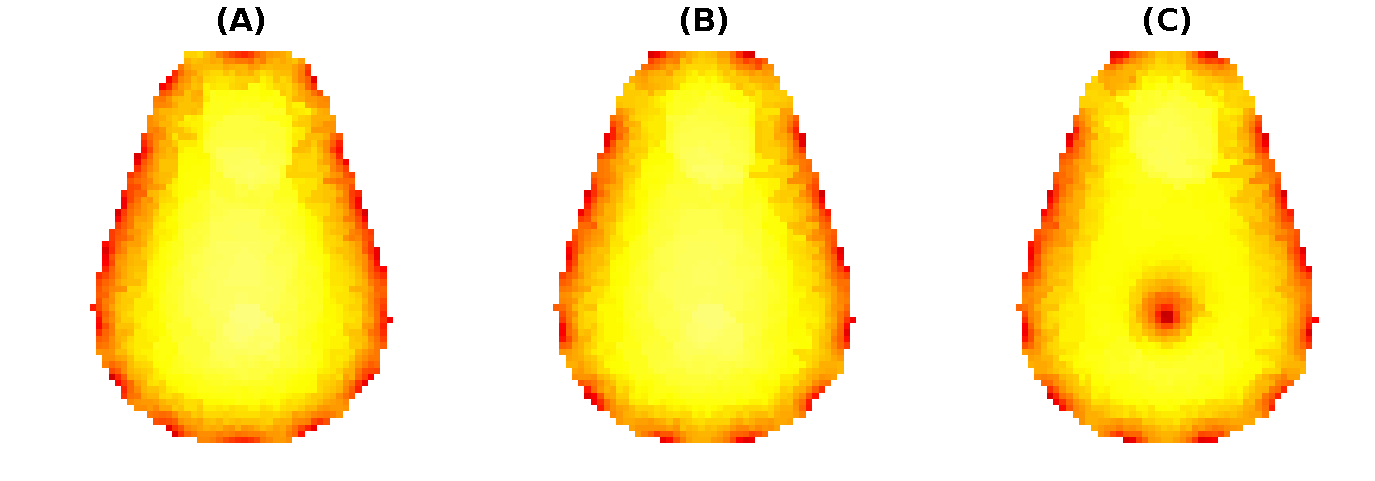
\includegraphics[width=.96\columnwidth]{chapter_5/imgs/lamb_sensitivity_profiles.pdf}
\caption[Sensitivity distribution in a lamb model]{\label{fig:sens_example}%
Sensitivity distribution averaged across 10 evenly spaced layers
between the electrode planes in the lamb model for: 
A) 32 external electrodes 
B) 28 external electrodes 
c) 28 external electrodes and 4 internal electrodes
}
\label{fig:sens_example}
\end{figure}

Images of one averaged breath per recording
were reconstructed using the 3D GREIT 
algorithm~\cite{bartek2016} which minimizes the effect
of electrode motion on the resulting image.
Results were compared for both 
external only and internal electrode configurations
using the same recording.
To obtain results with only external electrodes  all 
injections and measurements using internal electrodes 
were removed prior to reconstruction. 
Measurements on injecting electrodes were always removed.
Images from subject 3 during regular ventilation are 
shown  below in fig.~\ref{fig:img_example}.
With internal electrodes impedance changes at the cardiac frequency had a magnitude of 6.4\% \pm 4.35\%
of the ventilation frequency and without internal electrodes the amplitude of the cardiac frequency
was 0.8\% \pm 0.3\% of the ventilation frequency signal.
\begin{figure}
\centering
% Use the following line with your images (pdf preferred)
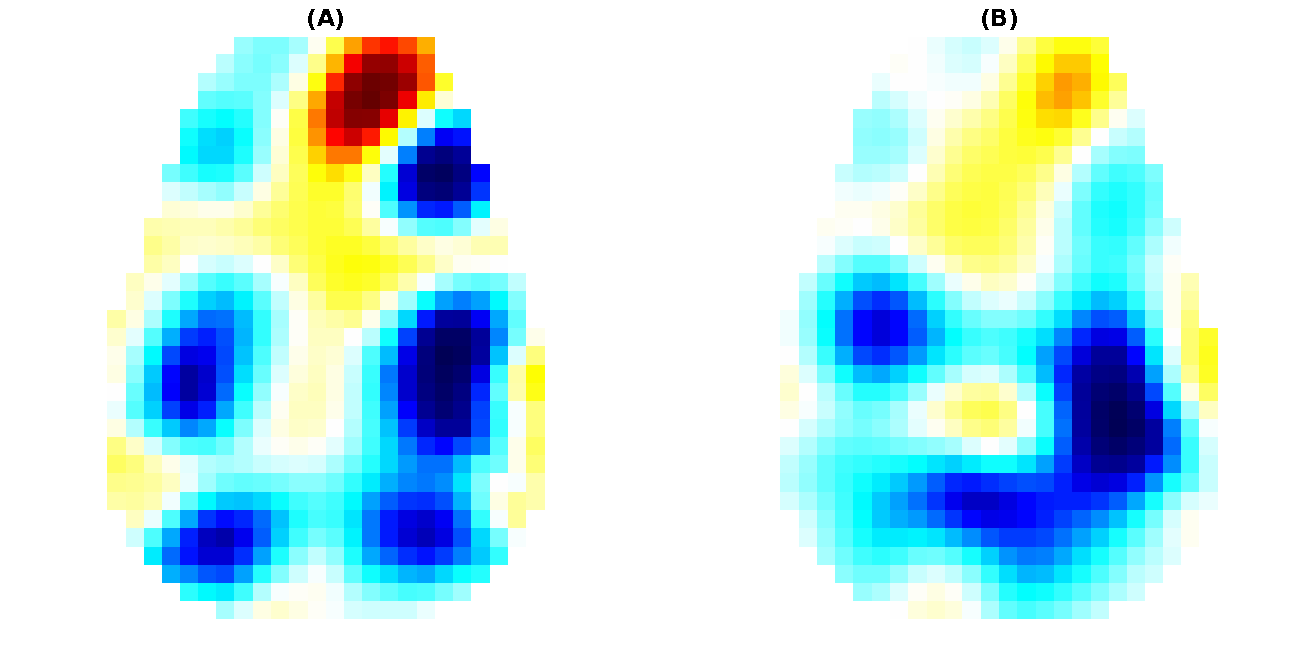
\includegraphics[width=.96\columnwidth]{chapter_5/imgs/lamb_imgs.pdf}
\caption[Reconstructed image of a single breath]{\label{fig:img_example}%
A single breath imaged with:
A) no current injections or measurements on internal
electrodes 
b) with internal electrodes
}
\label{fig:img_example}
\end{figure}
\section{Conclusions}
Reconstructions using the GREIT algorithm
with internal electrodes on 
an esophageal probe were able to give increased
sensitivity to cardiac-frequency impedance changes 
and may allow for better measures of blood pressure and pulse
wave velocity.   




\chapter{Conclusion}

\section{Summary of Findings}

\section{Future Work}

% BIBTEX
\phantomsection
\addcontentsline{toc}{chapter}{Bibliography}
\begin{singlespace}
  \setlength\bibitemsep{2pt}
  \printbibliography
\end{singlespace}

\appendix 
%\include{appendix/appendix_body}


\end{document}
